\باب{محافظ زاویہ نقشہ کشی}\شناخت{باب_محافظ_زاویہ_نقشہ_کشی}
اگر \عددی{z} سطح میں دائرہ کار \عددی{D} میں مخلوط تفاعل \عددی{w=f(z)} معین ہو، تب \عددی{D} میں ہر نقطہ کا مطابقتی نقطہ \عددی{w} سطح میں پایا جاتا ہے۔یوں \عددی{D}
 کا مطابقتی، \عددی{f(z)} کے سعت کا نقشہ، \عددی{w} سطح پر حاصل ہو گا۔جیومیٹریائی نقشہ ذہن میں تفاعل کی تصویر قائم کرتا ہے۔مختلف منحنیات اور خطوں کے نقوش دیکھ کر مخلوط تفاعل سمجھنے میں مدد ملتی ہے۔

جیسا ہم دیکھیں گے، اگر \عددی{f(z)} \ترچھا{تحلیلی} ہو تب \عددی{f(z)} سے حاصل نقشے میں زاویے تبدیل نہیں ہوں گے ماسوائے ان نقطوں پر جہاں \عددی{f'(z)=0} ہو۔ایسا نقشہ \اصطلاح{محافظ زاویہ نقشہ}\فرہنگ{محافظ زاویہ نقشہ}\فرہنگ{نقشہ!محافظ زاویہ}\حاشیہب{conformal map}\فرہنگ{conformal!map}\فرہنگ{mapping!conformal} کہلاتا ہے۔ 

\اصطلاح{محافظ زاویہ نقشہ گشی}\فرہنگ{محافظ زاویہ نقشہ کشی}\حاشیہب{conformal mapping}\فرہنگ{conformal!mapping} کے ذریعہ دیے گیے پیچیدہ خطے کا تبادل سادہ خطے میں کرتے ہوئے نظریہ مخفی قوہ کی دو بعدی سرحدی مسائل حل کیے جاتے ہیں۔اسی وجہ سے محافظ زاویہ نقشہ گشی انجینئری میں اہمیت رکھتی ہے۔

ہم نقشہ گشی کی تعریف پیش کرنے کے بعد نقشہ گشی کا عمل سکھائیں گے۔اس کے بعد کئی بنیادی تحلیلی تفاعل  کے نقوش پیش کریں گے۔عملی استعمال اس باب کے علاوہ باب \حوالہ{باب_مخلوط_تفاعل_اور_نظریہ_مخفی_قوہ} میں بھی پیش کیے جائیں گے۔

\حصہ{نقشہ گشی}\شناخت{حصہ_نقش_نقشہ_کشی}
حقیقی متغیرہ \عددی{x} کے حقیقی تفاعل \عددی{y=f(x)} کی منحنی  کو کارتیسی \عددی{xy} سطح پر  کھینچا جا سکتا ہے۔اس خط کو تفاعل کی \ترچھا{ترسیم} کہتے ہیں۔چونکہ مخلوط متغیرہ \عددی{z} کو جیومیٹریائی طور پر مخلوط سطح میں نقاط سے ظاہر کیا جاتا ہے اور یہی کچھ  \عددی{w} کے لئے بھی درست ہے لہٰذا مخلوط تفاعل
\begin{align}
w=f(z)=u(x,y)+iv(x,y)\quad \quad \quad (z=x+iy)
\end{align}
کی صورت حال زیادہ پیچیدہ ہے۔اس سے ہمیں خیال آتا ہے کہ ہم ان دو متغیرات کے لئے دو علیحدہ علیحدہ مخلوط سطحیں استعمال کریں۔ایک \عددی{z} سطح جس میں \عددی{z=x+iy} دکھایا جائے اور دوسری \عددی{w} سطح جس میں مطابقتی \عددی{w=u+iv} دکھایا جائے۔یوں  \عددی{f(z)} کی دائرہ کار \عددی{D} میں ہر \عددی{z}  کے لئے تفاعل \عددی{f(z)}  سطح \عددی{w}   میں قیمت \عددی{w=f(z)}  مختص کرے گا۔اس معین تعلق کو \عددی{f} کی دائرہ کار کی سطح \عددی{w} \اصطلاح{میں}\فرہنگ{میں}\حاشیہب{into}\فرہنگ{into}  \اصطلاح{نقشہ گشی}\فرہنگ{نقشہ گشی}\حاشیہب{mapping}\فرہنگ{mapping} (یا \ترچھا{تبادل}) کہتے ہیں، یا \عددی{f} کی دائرہ کار کا \عددی{f} کے سعت \اصطلاح{پر}\فرہنگ{پر}\حاشیہب{onto}\فرہنگ{onto} نقشہ کشی کہتے ہیں۔

\عددی{w_0=f(z_0)} جو نقطہ \عددی{z_0} کا مطابقتی نقطہ ہے،  \عددی{f(z)} کے لحاظ سے نقشے میں، \عددی{z_0} کا  \اصطلاح{عکس نقطہ}\فرہنگ{عکس نقطہ}\حاشیہب{image point}\فرہنگ{image!point} یا \اصطلاح{عکس}\فرہنگ{عکس}\حاشیہب{image}\فرہنگ{image} کہلاتا ہے۔ اگر \عددی{z} کسی منحنی پر حرکت کرے اور \عددی{f(z)} استمراری (نا کہ مستقل)  ہو تب مطابقتی نقطہ \عددی{w=f(z)} عمومی طور پر سطح \عددی{w} میں منحنی \عددی{C^*} پر حرکت کرے گا۔اس منحنی کو منحنی \عددی{C} کا عکس کہیں گے۔لفظ "عکس" کسی بھی نقطوں کے سلسلے اور خطہ کے لئے بھی استعمال کیا جاتا ہے۔ 

ہم دیکھیں گے کہ ایسی نقشہ کشی کی خواص کی تفتیش،  \عددی{z} سطح میں منحنیات اور خطے اور  \عددی{w} سطح میں ان کے عکس پر غور اور \عددی{w} سطح میں منحنیات اور خطے اور  \عددی{z} سطح میں ان کے عکس پر غور  کرنے سے  کی جا سکتی ہے۔ اس طرح  انفرادی نقطوں پر غور کرنے سے حاصل معلومات سے  زیادہ معلومات حاصل ہو گی۔

اگرچہ  \عددی{w} اور \عددی{z} کو دو علیحدہ علیحدہ سطحوں سے ظاہر کیا جاتا ہے، بعض اوقات یوں  سوچنا زیادہ بہتر ثابت ہوتا ہے  کہ اصل اور نقش ایک ہی سطح پر پائے جاتے ہوں اور  عمومی اصطلاحات مثلاً " گھومنا" اور "مستقیم حرکت" استعمال کرنا۔یوں \عددی{w=z+3}   مستقیم حرکت کہلائے گی جو \عددی{z} سطح میں ہر نقطہ کو دائیں جانب تین اکایاں منتقل کرتی ہے۔

تحلیل تفاعل \عددی{w=u+iv=f(z)} جس نقشہ کو ظاہر کرتا ہو، کی کسی مخصوص  خاصیت  جاننے کے لئے ہم \عددی{z} سطح میں سیدھے لکیروں \عددی{x=\text{مستقل}} اور \عددی{y=\text{مستقل}} کا \عددی{w} سطح میں عکس پر غور کر سکتے ہیں۔اسی طرح ہم دائرہ \عددی{\abs{z}=\text{مستقل}} یا مبدا سے گزرتی سیدھی لکیروں کی عکس پر غور کر سکتے ہیں۔اس کے علاوہ ہم \عددی{u(x,y)=\text{مستقل}} اور \عددی{v(x,y)=\text{مستقل}} منحنیات پر \عددی{z} سطح میں غور کر سکتے ہیں۔ان منحنیات کو \عددی{u} اور \عددی{v} کی \اصطلاح{ہموار منحنیات}\فرہنگ{ہموار!منحنی}\حاشیہب{level curves}\فرہنگ{curve!level} کہتے ہیں۔ ہم سادہ اشکال مثلاً چکور، تکون، مستطیل وغیرہ اور ان کے عکس پر بھی غور کر سکتے ہیں۔

آئیں چند مثالوں کی مدد سے ان حقائق کو بہتر سمجھنے کی کوشش کرتے ہیں۔

%====================
\ابتدا{مثال}\شناخت{مثال_نقش_خطی_مستقیم}\quad \موٹا{خطی تبادل \عددی{w=ax+b}}\\
درج ذیل نقش \اصطلاح{مستقیم حرکت} کو ظاہر کرتا ہے۔
\begin{align}\label{مساوات_نقش_خطی_مستقیم_الف}
w=z+b
\end{align}
شکل \حوالہ{شکل_مثال_نقش_خطی_مستقیم} میں مساوات \حوالہ{مساوات_نقش_خطی_مستقیم_الف} کو \عددی{w=z+2+i} کے لئے دکھایا گیا ہے جہاں مستطیل اور اس کا عکس دکھائے گئے ہیں جو یکساں ہیں (کیوں؟)۔\عددی{A} کا عکس \عددی{A^*}، وغیرہ۔زیادہ پیچیدہ اشکال میں نقطوں کو اس طرح ظاہر کرنا مفید ثابت ہوتا ہے۔ مساوات \حوالہ{مساوات_نقش_خطی_مستقیم_الف} میں \عددی{b=0} پر کرنے سے \اصطلاح{مماثل تبادل}\فرہنگ{تبادل!مماثل}\حاشیہب{identity transformation}\فرہنگ{transformation!identity} 
\begin{align*}
w=z
\end{align*}
حاصل ہوتا ہے جو ہر نقطے کو اپنے آپ پر نقش کرتا ہے۔
%
\begin{figure}
\centering
\begin{tikzpicture}
\draw(0,0)--++(3,0)node[below]{$x$};
\draw(0,0)node[below]{$0$}--++(0,2)node[right]{$y$};
\draw(1,0.5)node[left]{$A$}--++(0.5,0)node[right]{$B$}--++(0,1)node[right]{$C$}--++(-0.5,0)node[left]{$D$}--++(0,-1);
\foreach \x in {0.5,1,1.5,2,2.5}{\draw (\x,0)--++(0,0.1);}
\foreach \y in {0.5,1,1.5}{\draw (0,\y)--++(0.1,0);}
\draw(2,0)node[below]{$4$};
\draw(0,1)node[left]{$2$};
\draw(1.5,-0.5)node[below]{\text{\RL{($\,z$ مستوی)}}};
\begin{scope}[shift={(4cm,0)}]
\draw(0,0)--++(3,0)node[below]{$u$};
\draw(0,0)node[below]{$0$}--++(0,2)node[right]{$v$};
\draw(2,1)node[left]{$A^*$}--++(0.5,0)node[right]{$B^*$}--++(0,1)node[right]{$C^*$}--++(-0.5,0)node[left]{$D^*$}--++(0,-1);
\foreach \x in {0.5,1,1.5,2,2.5}{\draw (\x,0)--++(0,0.1);}
\foreach \y in {0.5,1,1.5}{\draw (0,\y)--++(0.1,0);}
\draw(2,0)node[below]{$4$};
\draw(0,1)node[left]{$2$};
\draw(1.5,-0.5)node[below]{\text{\RL{($\,w$ مستوی)}}};
\end{scope}
\end{tikzpicture}
\caption{مستقیم حرکت \عددی{w=z+2+i}}
\label{شکل_مثال_نقش_خطی_مستقیم}
\end{figure}

درج ذیل تبادل
\begin{align*}
w=az\quad \quad \quad (\abs{a}=1)
\end{align*}
مقررہ زاویہ \عددی{\phase{a}} سے گھومنے کو ظاہر کرتا ہے۔شکل \حوالہ{شکل_نقش_گھومنا} میں \عددی{w=iz} یعنی  گھڑی کی سوئیوں کی گھومنے کی الٹ رخ \عددی{\tfrac{\pi}{2}} زاویہ سے گھومنا دکھایا گیا ہے۔
\begin{figure}
\centering
\begin{tikzpicture}
\draw(0,0)--++(3,0)node[below]{$x$};
\draw(0,0)node[below]{$0$}--++(0,2.5)node[right]{$y$};
\draw([shift={(0:1)}]0,0) arc (0:90:1);
\draw([shift={(0:2)}]0,0) arc (0:90:2);
\draw[dashed](0,0)--++(30:2.5);
\draw[dashed](0,0)--++(60:2.5);
\foreach \x in {0.5,1,1.5,2,2.5}{\draw(\x,0)--++(0,0.1);}
\foreach \y in {0.5,1,1.5,2}{\draw(0,\y)--++(0.1,0);}
\draw(2.5,0)node[below]{$5$};
\draw(0,1.5)node[left]{$3$};
\draw(1,0)node[below]{$A$};
\draw(2,0)node[below]{$B$};
\draw(0,1)node[left]{$C$};
\draw(0,2)node[left]{$D$};
\draw(1.5,-0.5)node[below]{\text{\RL{($\,z$ مستوی)}}};
%
\begin{scope}[xshift={8cm}]
\draw(-3,0)--(0.75,0)node[below]{$u$};
\draw(0,0)node[below]{$0$}--++(0,2.5)node[right]{$v$};
\draw([shift={(90:1)}]0,0) arc (90:180:1);
\draw([shift={(90:2)}]0,0) arc (90:180:2);
\draw[dashed](0,0)--++(120:2.5);
\draw[dashed](0,0)--++(150:2.5);
\foreach \x in {0.5,-0.5,-1,-1.5,-2,-2.5}{\draw(\x,0)--++(0,0.1);}
\foreach \y in {0.5,1,1.5,2}{\draw(0,\y)--++(0.1,0);}
\draw(-2.5,0.1)node[above]{$-5$};
\draw(0.1,1.5)node[right]{$3$};
\draw(0,1)node[right]{$A^*$};
\draw(0,2)node[right]{$B^*$};
\draw(-1,0)node[below]{$C^*$};
\draw(-2,0)node[below]{$D^*$};
\draw(-1.5,-0.5)node[below]{\text{\RL{($\,w$ مستوی)}}};
\end{scope}
\end{tikzpicture}
\caption{گھڑی کی الٹ رخ گھومنے کا زاویہ \عددی{\tfrac{\pi}{2}} ہے۔}
\label{شکل_نقش_گھومنا}
\end{figure}

درج ذیل تبادل
\begin{align*}
w=az \quad \quad \quad (\text{\RL{مثبت حقیقی $a$}})
\end{align*}
میں \عددی{a>1} اتساع جبکہ \عددی{0<a<1} سکڑاو کو ظاہر کرتا ہے۔اسی طرح 
\begin{align}
w=az\quad \quad \quad (\text{\RL{اختیاری $a$}})
\end{align}
زاویہ \عددی{\phase{a}} سے گھومنے کو اور ساتھ ہی یکساں اتساع یا سکڑاو کو ظاہر کرتا ہے۔ درج ذیل تبادل
\begin{align}
w=az+b
\end{align}
\اصطلاح{خطی تبادل}\فرہنگ{تبادل!خطی}\حاشیہب{linear transformation}\فرہنگ{transformation!linear} کہلاتا ہے جو گھومنے کے ساتھ اتساع یا سکڑاو \عددی{w_1=az} کے ساتھ ساتھ مستقیم حرکت \عددی{w=w_1+b} کو ظاہر کرتا ہے۔ شکل \حوالہ{شکل_نقش_خطی_تبادل} میں \عددی{w=(1+i)z+2i} تبادل دکھایا گیا ہے جو گھڑی کی الٹ رخ  \عددی{\tfrac{\pi}{4}} زاویے کے گھومنے اور \عددی{\abs{1+i}=\sqrt{2}} تناسب کی اتساع کے بعد اوپر کی رخ مستقیم حرکت کو ظاہر کرتا ہے۔  
\begin{figure}
\centering
\begin{tikzpicture}
\draw(0,0)--++(2,0)node[below]{$x$};
\draw(0,0)--++(0,2)node[left]{$y$};
\draw([shift={(0:0.5)}]0,0) arc (0:90:0.5);
\draw([shift={(0:1)}]0,0) arc (0:90:1);
\draw([shift={(0:1.5)}]0,0) arc (0:90:1.5);
\draw(0.5,0)node[below]{$1$};
\draw(1,0)node[below]{$2$};
\draw(1.5,0)node[below]{$3$};
\draw(0,0.5)node[left]{$1$};
\draw(0,1)node[left]{$2$};
\draw(0,1.5)node[left]{$3$};
\draw[thick](0,0)--++(1.5,0)node[shift={(0.2,0.2)}]{$B$};
\draw[thick](0,0)node[shift={(0.2,0.2)}]{$A$}--++(0,1.5)node[shift={(0.2,0.2)}]{$C$};
\draw(1,-1)node[]{$z=x+iy$};
\draw(1,-1.5)node[]{\text{\RL{($\,z$ مستوی)}}};
\draw(0,0)node[below]{$0$}node[left]{$0$};
\begin{scope}[xshift={(4cm)}]
\draw(-1.5,0)--(1.5,0)node[below]{$u_1$};
\draw(0,0)--++(0,2.75)node[right]{$v_1$};
\draw([shift={(45:0.707)}]0,0) arc (45:135:0.707);
\draw([shift={(45:1.4142)}]0,0) arc (45:135:1.4142);
\draw([shift={(45:2.121)}]0,0) arc (45:135:2.121);
\draw(0,0)node[below]{$0$};
\draw[thick](0,0)node[shift={(0.5,0.2)}]{$A^*$}--++(45:2.212)node[right]{$B^*$};
\draw[thick](0,0)--++(135:2.212)node[left]{$C^*$};
\foreach \x in {-1,-0.5,1}{\draw(\x,0)--++(0,0.1);}
\foreach \y in {0.5,1,1.5,2,2.5}{\draw(0,\y)--++(0.1,0);}
\draw(0,2.5)node[left]{$5$};
\draw(1,-1)node[]{$w_1=u_1+iv_1$};
\draw(1,-1.5)node[]{\text{\RL{($\,w_1$ مستوی)}}};
\end{scope}
\begin{scope}[xshift={(8cm)}]
\draw(-1.5,0)--(1.5,0)node[below]{$u$};
\draw(0,0)--++(0,3.75)node[right]{$v$};
\draw([shift={(45:0.707)}]0,1) arc (45:135:0.707);
\draw([shift={(45:1.4142)}]0,1) arc (45:135:1.4142);
\draw([shift={(45:2.121)}]0,1) arc (45:135:2.121);
\draw(0,0)node[below]{$0$};
\draw[thick](0,1)node[shift={(0.5,0.2)}]{$A^{**}$}--++(45:2.212)node[right]{$B^{**}$};
\draw[thick](0,1)--++(135:2.212)node[left]{$C^{**}$};
\foreach \x in {-1,-0.5,0.5,1}{\draw(\x,0)--++(0,0.1);}
\foreach \y in {0.5,1,1.5,2,2.5,3.5}{\draw(0,\y)--++(0.1,0);}
\draw(0,2.6)node[left]{$5$};
\draw(1,-1)node[]{$w=u+iv$};
\draw(1,-1.5)node[]{\text{\RL{($\,w$ مستوی)}}};
\end{scope}
\end{tikzpicture}
\caption{خطی تبادل $w=(1+i)z+2i$ جس میں  گھومنا،  اتساع $w_1=(1+i)z$ اور مستقیم حرکت $w=w_1+2i$ شامل ہے۔}
\label{شکل_نقش_خطی_تبادل}
\end{figure}
\انتہا{مثال}
%========================
\ابتدا{مثال}\شناخت{مثال_نقش_مربع}\quad \موٹا{نقش \عددی{w=z^2}}\\
ہم درج ذیل نقش پر غور کرنا چاہتے ہیں۔
\begin{align}\label{مساوات_نقش_مربع_الف}
w=z^2
\end{align}
یہاں قطبی محدد استعمال کرنا بہتر ثابت ہوتا ہے۔یوں \عددی{z=e^{i\theta}} اور \عددی{w=Re^{i\phi}} لیتے ہوئے  مساوات \حوالہ{مساوات_نقش_مربع_الف} \عددی{Re^{i\phi}=r^2e^{i2\theta}} لکھی جائے گی جس سے 
\begin{align*}
R=r^2,\quad \phi=2\theta
\end{align*}
حاصل ہوتے ہیں۔ یوں دائروں \عددی{r=r_0=\text{مستقل}} کا نقش دائرے \عددی{R=r_0^2=\text{مستقل}} ہوں گے جبکہ مبدا سے گزرتی سیدھی لکیروں \عددی{\theta=\theta_0=\text{مستقل}} کا نقش دگنی زاویہ پر لکیریں \عددی{\phi=2\theta_0=\text{مستقل}} ہوں گی۔ خاص کر \عددی{z} سطح میں مثبت حقیقی محور \عددی{(\theta=0)} کا نقش \عددی{w} سطح میں مثبت حقیقی محور ہو گا جبکہ \عددی{z} سطح میں مثبت خیالی محور \عددی{\theta=\tfrac{\pi}{2}} کا نقش \عددی{w} سطح میں منفی حقیقی محور ہو گا۔ یہ نقش  مبدا پر ہر زاویہ کو دگنا کرتا ہے۔ربع اول \عددی{0\le \theta \le \tfrac{\pi}{2}} کا نقش بالائی نصف \عددی{w} سطح ہو گی (شکل \حوالہ{شکل_نقش_مربع})۔
\begin{figure}
\centering
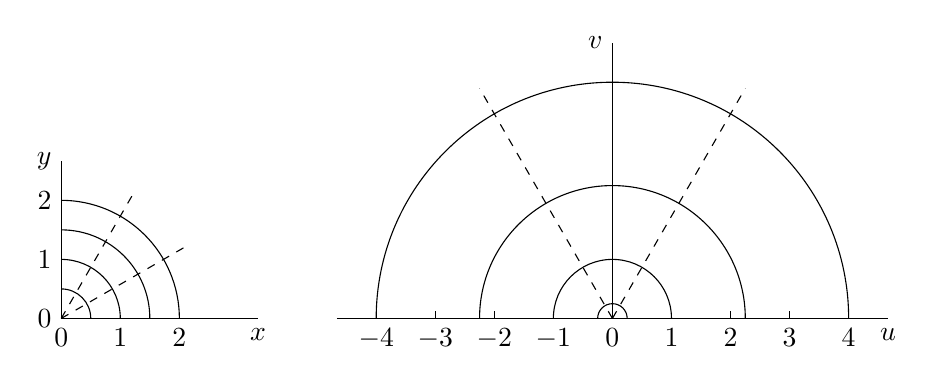
\begin{tikzpicture}
\pgfmathsetmacro{\len}{3/4}
\draw(0,0)--++(2.5,0)node[below]{$x$};
\draw(0,0)--++(0,2)node[left]{$y$};
\draw([shift={(0:0.5*\len)}]0,0) arc (0:90:0.5*\len);
\draw([shift={(0:1*\len)}]0,0) arc (0:90:1*\len);
\draw([shift={(0:1.5*\len)}]0,0) arc (0:90:1.5*\len);
\draw([shift={(0:2*\len)}]0,0) arc (0:90:2*\len);
\draw(1*\len,0)node[below]{$1$};
\draw(2*\len,0)node[below]{$2$};
\draw(0,1*\len)node[left]{$1$};
\draw(0,2*\len)node[left]{$2$};
\draw[dashed](0,0)--++(30:2.5*\len);
\draw[dashed](0,0)node[below]{$0$}node[left]{$0$}--++(60:2.5*\len);
\begin{scope}[xshift={(7cm)}]
\draw(-3.5,0)--(3.5,0)node[below]{$u$};
\draw(0,0)--++(0,3.5)node[left]{$v$};
\draw([shift={(0:0.25*\len)}]0,0) arc (0:180:0.25*\len);
\draw([shift={(0:1*\len)}]0,0) arc (0:180:1*\len);
\draw([shift={(0:2.25*\len)}]0,0) arc (0:180:2.25*\len);
\draw([shift={(0:4*\len)}]0,0) arc (0:180:4*\len);
\foreach \x in {-3,-2,2,3}{\draw(\x*\len,0)--++(0,0.1);}
\draw(1*\len,0)node[below]{$1$};
\draw(2*\len,0)node[below]{$2$};
\draw(3*\len,0)node[below]{$3$};
\draw(4*\len,0)node[below]{$4$};
\draw(-1*\len,0)node[below]{$-1$};
\draw(-2*\len,0)node[below]{$-2$};
\draw(-3*\len,0)node[below]{$-3$};
\draw(-4*\len,0)node[below]{$-4$};
\draw[dashed](0,0)node[below]{$0$}--++(60:4.5*\len);
\draw[dashed](0,0)--++(120:4.5*\len);
\end{scope}
\end{tikzpicture}
\caption{نقش \عددی{w=z^2}}
\label{شکل_نقش_مربع}
\end{figure}

مستطیل محدد میں تبادل \عددی{w=z^2} درج ذیل دے گا۔
\begin{align*}
u+iv=x^2-y^2+i2xy
\end{align*}
حقیقی اور خیالی اجزاء علیحدہ کرتے ہوئے 
\begin{align}\label{مساوات_نقش_مربع_ب}
u=x^2-y^2,\quad v=2xy
\end{align}
ملتا ہے۔ہم دیکھتے ہیں کہ \عددی{u} اور \عددی{v} کی \اصطلاح{ہموار سطحات}\فرہنگ{ہموار!سطح}\فرہنگ{سطح!ہموار} متساوی الاضلاع قطع زائد ہوں گے جن کی متقارب لکیریں\فرہنگ{متقارب!لکیریں}\حاشیہب{asymptotes} \عددی{y=\mp x} اور محدد کی محور ہیں۔ہم دیکھتے ہیں مساوات \حوالہ{مساوات_نقش_مربع_ب} میں دیے گئے  خطوط ایک دوسرے کی عمودی مطقاطع خطوط (حصہ \حوالہ{حصہ_درجہ_اول_عمودی_خطوط_کی_نسلیں}) ہیں۔ شکل \حوالہ{شکل_نقش_مربع_ہموار_سطحیں} میں \عددی{z} سطح میں دو خطے \عددی{w} سطح میں مستطیل پر نقش ہوں گے۔ظاہر ہے کہ ہر نقطہ \عددی{w\ne 0} سطح \عددی{z} میں ٹھیک  دو نقطوں کا عکس ہو گا۔

ہم مساوات \حوالہ{مساوات_نقش_مربع_ب} استعمال کرتے ہوئے سیدھی خطوط \عددی{x=\text{مستقل}} اور \عددی{y=\text{مستقل}} کا عکس تلاش کر سکتے ہیں۔خط \عددی{x=c=\text{مستقل}} کا عکس
\begin{align*}
u=c^2-y^2,\quad v=2cy
\end{align*}
سے \عددی{y} حذف کرتے ہوئے
\begin{align*}
v^2=4c^2(c^2-u)
\end{align*}
حاصل ہوتا ہے جو قطع مکافی کو ظاہر کرتی ہے جو بائیں رخ کھلتا ہے۔مبدا اس قطع مکافی کا ماسکہ ہو گا۔اسی طرح \عددی{y=k=\text{مستقل}} کا عکس
\begin{align*}
v^2=4k^2(k^2+u)
\end{align*}
ہو گا جو دائیں کو کھلتا ہوا قطع مکافی ہے جس کا ماسکہ عین مبدا پر ہے (شکل \حوالہ{شکل_نقش_مربع_نقش_میں_سیدھے_خطوط_کا_عکس})۔
\begin{figure}
\centering
\begin{tikzpicture}
\begin{axis}[small,clip=false,axis lines*=middle,ymin=-3,ymax=3,xmin=-3,xmax=3.5,xtick={-1,1},ytick={-1,1},xticklabels={$-1$,$1$},yticklabels={$-1$,$1$},xlabel={$x$},ylabel={$y$},ylabel style={rotate=-90},xlabel style={at={(current axis.right of origin)},anchor=west},ylabel style={at={(current axis.above origin)},anchor=south}]
\shade[fill=gray!20!white](axis cs: 1.53,0.64)--(axis cs:1.7989,1.1118)--(axis cs: 2.236,0.8944)--(axis cs:2.05817,0.4858)--(axis cs: 1.53,0.64);
\shade[fill=gray!20!white](axis cs: 2.236,0.8944)--(axis cs:2.05817,0.4858)--(axis cs:2.48239,0.402837)--(axis cs:2.57,0.7782)--(axis cs:2.236,0.8944);
%
\shade[fill=gray!20!white](axis cs: -1.53,-0.64)--(axis cs:-1.7989,-1.1118)--(axis cs: -2.236,-0.8944)--(axis cs:-2.05817,-0.4858)--(axis cs: -1.53,-0.64);
\shade[fill=gray!20!white](axis cs: -2.236,-0.8944)--(axis cs:-2.05817,-0.4858)--(axis cs:-2.48239,-0.402837)--(axis cs:-2.57,-0.7782)--(axis cs:-2.236,-0.8944);
%
\addplot[domain=-2:2]{sqrt(x^2-0)}node[pin=30:{$u=0$}]{};
\addplot[domain=-2:2,name path=ut]{sqrt(x^2+2)};
\addplot[domain=-2:2,name path=uf]{sqrt(x^2+4)};
\addplot[domain=-2:2]{sqrt(x^2+6)}node[pin=30:{$u=-6$}]{};
%
\addplot[domain=-2:2]{-sqrt(x^2-0)};
\addplot[domain=-2:2]{-sqrt(x^2+2)};
\addplot[domain=-2:2]{-sqrt(x^2+4)};
\addplot[domain=-2:2]{-sqrt(x^2+6)};
%
\addplot[domain=-2:2]({sqrt(2+x^2)},{x});
\addplot[domain=-2:2]({sqrt(4+x^2)},{x});
\addplot[domain=-2:2]({sqrt(6+x^2)},{x})node[pin=0:{$u=6$}]{};
%
\addplot[domain=-2:2]({-sqrt(2+x^2)},{x});
\addplot[domain=-2:2]({-sqrt(4+x^2)},{x});
\addplot[domain=-2:2]({-sqrt(6+x^2)},{x});
%%
\addplot[domain=0.35:3,dashed,name path=vt]({x},{2/(2*x)})node[pin={[pin edge=solid]0:{$v=2$}}]{};
\addplot[domain=0.7:3,dashed,name path=vf]({x},{4/(2*x)});
\addplot[domain=1.05:3,dashed]({x},{6/(2*x)})node[pin={[pin edge=solid]0:{$v=6$}}]{};
%
\addplot[domain=0.35:3,dashed]({x},{-2/(2*x)});
\addplot[domain=0.7:3,dashed]({x},{-4/(2*x)});
\addplot[domain=1.05:3,dashed]({x},{-6/(2*x)})node[solid,pin={[pin distance=0.25cm,pin edge=solid]0:{$v=-6$}}]{};
%
\addplot[domain=0.35:3,dashed](-{x},{2/(2*x)});
\addplot[domain=0.7:3,dashed](-{x},{4/(2*x)});
\addplot[domain=1.05:3,dashed](-{x},{6/(2*x)});
%
\addplot[domain=0.35:3,dashed](-{x},{-2/(2*x)});
\addplot[domain=0.7:3,dashed](-{x},{-4/(2*x)});
\addplot[domain=1.05:3,dashed](-{x},{-6/(2*x)});
\end{axis}
\begin{scope}[shift={(8cm,2cm)}]
\pgfmathsetmacro{\kk}{0.25}
\draw[dashed](-4.5*\kk,0)--(4.5*\kk,0)node[right]{$u$};
\draw(0,-4.5*\kk)--(0,4.5*\kk)node[above]{$v$};
%
\shade[gray!20!white](1*\kk,1*\kk)--++(2*\kk,0)--++(0,1*\kk)--++(-2*\kk,0)--++(0,-1*\kk);
%
\foreach \x in {-4,-3,-2,-1,1,2,3,4}{\draw(\x*\kk,-4.5*\kk)--++(0,9*\kk);}
\foreach \y in {-4,-3,-2,-1,1,2,3,4}{\draw[dashed](-4.5*\kk,\y*\kk)--++(9*\kk,0);}
\draw(0,0)node[ocirc]{};
\end{scope}
\end{tikzpicture}
\caption{نقش $w=z^2$ کی صورت میں $u$ اور $v$ کی ہموار سطحیں}
\label{شکل_نقش_مربع_ہموار_سطحیں}
\end{figure}
%
\begin{figure}
\centering
\begin{tikzpicture}
\begin{axis}[small,clip=false,axis lines*=middle,ymin=-5,ymax=5,xmin=-5.5,xmax=5.5,xtick={-2,-3,-5,2,3,5},xticklabels={$-2$,$-3$,$-5$,$2$,$3$,$5$},ytick={-4,-2,2,4},yticklabels={$-4$,$-2$,$2$,$4$},xlabel style={at={(current axis.right of origin)},anchor=west},ylabel style={rotate=-90},ylabel style={at={(current axis.above origin)},anchor=west},xlabel={$u$},ylabel={$v$}]
\addplot[dashed,domain=-2.3:2.3] ({0.5^2-x^2/(4*0.5^2)},{x})node[pos=0,left]{$x=\tfrac{1}{2}$};
\addplot[dashed,domain=-5:5] ({1^2-x^2/(4*1^2)},{x})node[pos=0,left]{$x=1$};
\addplot[dashed,domain=-3.5:3.5] ({1.5^2-x^2/(4*1.5^2)},{x});
\addplot[dashed,domain=-5:5] ({2^2-x^2/(4*2^2)},{x})node[pos=0,below]{$x=2$};
%
\addplot[domain=-2.2:2.2] ({x^2/(4*0.5^2)-0.5^2},{x})node[right]{$y=\tfrac{1}{2}$};
\addplot[smooth,domain=-4.5:4.5] ({x^2/(4*1^2)-1^2},{x})node[right]{$y=1$};
\addplot[domain=-3.6:3.6] ({x^2/(4*1.5^2)-1.5^2},{x});
\addplot[domain=-4.5:4.5] ({x^2/(4*2^2)-2^2},{x})node[above]{$y=2$};
\end{axis}
\end{tikzpicture}
\caption{نقش \عددی{w=z^2} میں سیدھے خطوط \عددی{x=c} اور \عددی{y=c^*} کے عکس}
\label{شکل_نقش_مربع_نقش_میں_سیدھے_خطوط_کا_عکس}
\end{figure}
\انتہا{مثال}
%===========================
باقی طاقت
\begin{align}
w=z^n,\quad n=3,4,\cdots
\end{align}
پر بھی اسی طرح غور کیا جا سکتا ہے۔ظاہر ہے کہ ان کی ہموار سطحات کی مساوات مزید پیچیدہ ہوں گی۔زاویائی خطہ \عددی{0\le \phase{z} \le \tfrac{\pi}{n}} بالائی نصف \عددی{w} سطح پر نقش ہو گا (شکل \حوالہ{شکل_نقش_عمومی_طاقت})۔

منفی طاقت کی نقش \عددی{\tfrac{1}{z},\tfrac{1}{z^2},\cdots} پر بھی قطبی محدد کی مدد سے غور کیا جا سکتا ہے۔عملاً اہم ترین صورت درج ذیل مثال میں دی گئی ہے۔
\begin{figure}
\centering
\begin{tikzpicture}
\draw(0,0)--++(2,0)node[below]{$x$};
\draw(0,0)--++(0,1)node[left]{$y$};
\draw(0,0)--++(30:1.5);
\draw[-stealth]([shift={(0:0.5)}]0,0) arc (0:30:0.5);
\draw(15:0.9)node{$\tfrac{\pi}{n}$};
%
\begin{scope}[xshift={(6cm)}]
\draw(-2,0)--(2,0)node[below]{$u$};
\draw(0,0)--++(0,1)node[right]{$v$};
\end{scope}
\end{tikzpicture}
\caption{نقش $w=z^n\,$}
\label{شکل_نقش_عمومی_طاقت}
\end{figure}

%=========================
\ابتدا{مثال}\شناخت{مثال_نقش_الٹ_جانا}\quad \موٹا{نقش $w=\tfrac{1}{z}$۔ الٹ جانا}\\
ہم درج ذیل نقش پر غور کرتے ہیں۔
\begin{align}\label{مساوات_نقش_الٹ_جانا_الف}
w=\frac{1}{z}\quad \quad \quad z\ne 0
\end{align}
قطبی محدد استعمال کرتے ہوئے \عددی{z=re^{i\theta}} اور \عددی{w=Re^{i\phi}} لکھتے ہیں۔یوں مساوات \حوالہ{مساوات_نقش_الٹ_جانا_الف} سے
\begin{align}
R=\frac{1}{r},\quad \phi=-\theta\quad \quad \quad (r\ne 0)
\end{align}
حاصل ہوتا ہے۔اس سے ہم دیکھتے ہیں کہ نقطہ \عددی{w=\tfrac{1}{z}\,(z\ne 0)}، مبدا سے نکلتی سیدھی لکیر جو \عددی{\bar{z}} سے گزرتی ہو پر واقع ہے۔مبدا سے اس نقطے کا فاصلہ \عددی{\tfrac{1}{\abs{z}}} ہے۔

جیومیٹریائی طور پر \عددی{z} کو اکائی دائرے میں الٹاتے ہوئے اس کا \عددی{x} محور میں عکس لینے سے \عددی{w=\tfrac{1}{z}}  حاصل ہو گا۔آپ متشابہ مثلثات  استعمال کرتے ہوئے اس حقیقت کو ثابت کر سکتے ہیں (شکل  \حوالہ{شکل_نقش_اکائی_دائرے_میں_الٹ})۔

شکل \حوالہ{شکل_نقش_مثال_الٹ} میں دکھایا گیا ہے کہ \عددی{w=\tfrac{1}{z}} نقش،  افقی اور کھڑی سیدھی لکیروں کو دائروں یا سیدھی لکیروں پر عکس کرتی ہے۔یہاں تک کہ درج ذیل جملہ ہر صورت درست ہو گا۔\\
\ترچھا{\عددی{w=\tfrac{1}{z}} ہر سیدھی لکیر یا دائرے کو دائرے یا سیدھے لکیر پر نقش کرتا ہے۔}\\
ثبوت: \عددی{z} سطح میں ہر سیدھی لکیر یا دائرہ کو درج ذیل مساوات ظاہر کرتی ہے۔
\begin{align*}
A(x^2+y^2)+Bx+Cy+D=0\quad \quad (A,B,C,D \text{حقیقی})
\end{align*}
\عددی{A=0} سیدھی لکیر دیتی ہے جبکہ \عددی{A\ne 0} دائرہ دیتی ہے۔ \عددی{z} اور \عددی{\bar{z}}  استعمال کرتے ہوئے اس مساوات کو درج ذیل لکھا جا سکتا ہے۔
\begin{align*}
Az\bar{z}+B\frac{z+\bar{z}}{2}+C\frac{z-\bar{z}}{i2}+D=0
\end{align*}
چونکہ \عددی{w=\tfrac{1}{z}} ہے لہٰذا اس میں \عددی{z=\tfrac{1}{w}} پر کرتے ہوئے \عددی{w\bar{w}} سے ضرب دینے سے 
\begin{align*}
A+B\frac{w+\bar{w}}{2}+C\frac{\bar{w}-w}{i2}+Dw\bar{w}=0
\end{align*}
حاصل ہوتا ہے جس کو \عددی{u} اور \عددی{v} کی صورت میں لکھتے ہوئے
\begin{align*}
A+Bu-Cv+D(u^2+v^2)=0
\end{align*}
حاصل ہوتا ہے جو \عددی{D\ne 0} کی صورت میں دائرہ ہو گا جبکہ \عددی{D=0} کی صورت میں \عددی{w} سطح میں سیدھی لکیر ہو گی۔ 
\begin{figure}
\centering
\begin{tikzpicture}
\draw(-1.5,0)--(2,0)node[right]{$x$};
\draw(0,0) circle (1);
\draw[dashed](0,0)--(-20:1)coordinate(kA);
\draw[dashed](0,0)--(100:1)coordinate(kB);
\path[name path=kkA](kA)--++(-20+90:-1)coordinate(kC)--++(-20+90:2.75);
\path[name path=kkB](kB)--++(100-90:-1)coordinate(kD)--++(100-90:2.75);
\draw[name path=kkC](kA)--(kB);
\draw[name intersections={of=kkA and kkB}] (kC)--(intersection-1)coordinate(kkE);
\draw(kD)--(intersection-1);
\draw[name path=kkD](0,0)--(kkE)node[ocirc]{}node[right]{$z$};
\path[name intersections={of=kkC and kkD}];
\draw(intersection-1)node[ocirc]{}node[above]{$\bar{w}$};
\draw(0,0)node[ocirc]{}node[below]{$0$};
\draw(kA)node[ocirc]{}node[right]{$N_2$};
\draw(kB)node[ocirc]{}node[above]{$N_1$};
\draw(1,0)node[shift={(-0.15,0.2)}]{$1$};
\end{tikzpicture}
\caption{$z$ سے $w=\tfrac{1}{z}$ کا جیومیٹریائی حصول۔ نقطہ \عددی{z} سے اکائی دائرے تک مماس،  دائرے کو $N_1$ اور $N_2$ پر چھوتے ہیں۔مبدا سے $z$ تک لکیر اور $N_1$ سے $N_2$ تک لکیر نقطہ $\bar{w}$ پر ایک دوسرے کو قطع کرتے ہیں۔ }
\label{شکل_نقش_اکائی_دائرے_میں_الٹ}
\end{figure}
%

\begin{figure}
\centering
\begin{subfigure}{0.5\textwidth}
\centering
\begin{tikzpicture}
\draw(-2.25,0)--(1.5,0)node[right]{$x$};
\draw(0,-1.25)--(0,1.5)node[right]{$y$};
\draw(0,0)node[ocirc]{};
%
\foreach \x in {-0.5,0.5,1}{\draw(\x,-1.25)--(\x,1.25);}
\foreach \y in {-1,-0.5,0.5,1}{\draw(-2.25,\y)--(1.5,\y);}
\draw(-1,-1.25)--(-1,-0.48) (-1,-0.1)--(-1,1.25);
\draw(-2,-1.25)--(-2,-0.48) (-2,-0.1)--(-2,1.25);
\draw(0,1)node[shift={(-0.25,0)},fill=white]{$1$};
\draw(0,-1)node[shift={(-0.4,0)},fill=white]{$-1$};
\draw(1,0)node[below,fill=white]{$1$};
\draw(-1,0)node[shift={(-0.15,-0.25)}]{$-1$};
\draw(-2,0)node[shift={(-0.15,-0.25)}]{$-2$};
%
\draw[fill=black] (-2,0.5)--++(1,0)--++(0,0.5)--++(-1,0)--++(0,-0.5);
\draw[fill=gray] (0.5,-0.5)--++(0.5,0)--++(0,-0.5)--++(-0.5,0)--++(0,0.5);
\end{tikzpicture}
\end{subfigure}%
\begin{subfigure}{0.5\textwidth}
\centering
\def\ringa{(0,-1) circle (1) (0,-1/2) circle (1/2)}
\def\ringb{(-1/2,0) circle (1/2) (-1/4,0) circle (1/4)}
\def\ringc{(0,1) circle (1) (0,1/2) circle (1/2)}
\def\ringd{(1,0) circle (1) (1/2,0) circle (1/2)}
\begin{tikzpicture}%[z={(-0.5cm,-0.5cm)},x={(1cm,0cm)},y={(0cm,1cm)}]

  \begin{scope}[even odd rule]
        % Define a clipping path. All paths outside ringa will
        % be cut because the even odd rule is set. 
        \clip \ringa;
        % Fill ringb. Since the even odd rule is set, only the
        % ring will be filled, not the hole in the middle.  
        \fill[fill=black] \ringb;
    \end{scope}
   \begin{scope}[even odd rule]
        % Define a clipping path. All paths outside ringa will
        % be cut because the even odd rule is set. 
        \clip \ringc;
        % Fill ringb. Since the even odd rule is set, only the
        % ring will be filled, not the hole in the middle.  
        \fill[fill=gray] \ringd;
    \end{scope}
%
\draw(-2.25,0)--(3,0)node[below]{$u$};
\draw(0,-3)--(0,3)node[left]{$v$};
%
\draw (1,0) circle (1); %x=-1/2
\draw (-1,0) circle (1); %x=1/2
\draw (1/2,0) circle (1/2); %x=-1
\draw (-1/2,0) circle (1/2); %x=1
\draw (1/4,0) circle (1/4); %x=-2
\draw (-1/4,0) circle (1/4); %x=2
%
\draw (0,1) circle (1); %y=-1/2
\draw (0,-1) circle (1); %y=1/2
\draw (0,1/2) circle (1/2); %y=-1
\draw (0,-1/2) circle (1/2); %y=1
%
\draw[stealth-](1,0)++(60:1) to [out=60,in=-145]++(0.2,0.2)node[above]{$x=\tfrac{1}{2}$};
\draw[stealth-](-1,0)++(115:1) to [out=130,in=-70]++(-0.3,0.3)node[above]{$x=-\tfrac{1}{2}$};
\draw[stealth-](0,1)++(45:1) to [out=60,in=180]++(0.3,0.3)node[right]{$y=-\tfrac{1}{2}$};
\draw[stealth-](0,-1)++(-135:1) to [out=-120,in=20]++(-0.3,-0.3)node[left]{$y=\tfrac{1}{2}$};
%
\draw(0,1)node[shift={(-0.2,0.2)}]{$1$};
\draw(0,-1)node[shift={(-0.3,-0.2)}]{$-1$};
\draw(1,0)node[shift={(0.2,-0.2)}]{$1$};
\draw(-1,0)node[shift={(-0.3,-0.2)}]{$-1$};
%
\draw(0,2)node[shift={(-0.2,0.2)}]{$2$};
\draw(0,-2)node[shift={(-0.3,-0.2)}]{$-2$};
\draw(2,0)node[shift={(0.2,-0.2)}]{$2$};
\draw(-2,0)node[shift={(-0.3,-0.2)}]{$-2$};
%text
\draw[stealth-](0,-2.5) to [out=20,in=180]++(0.3,0.1)node[right]{$x=0$};
\draw[stealth-](2.25,0) to [out=60,in=-145]++(0.3,0.3)node[above]{$y=0$};
\end{tikzpicture}%
\end{subfigure}%
\caption{نقش \عددی{w=\tfrac{1}{z}}}
\label{شکل_نقش_مثال_الٹ}
\end{figure}
\انتہا{مثال}
%===========================

\حصہء{سوالات}
سوال \حوالہ{سوال_نقش_عکس_دکھائیں_الف} تا سوال \حوالہ{سوال_نقش_عکس_دکھائیں_پ} میں زیر نقش \عددی{w=(1-i)z+2} دیے گئے منحنیات یا خطوں کا عکس تلاش کریں۔عکس کو \عددی{w} سطح پر دکھائیں۔

%==============
\ابتدا{سوال}\شناخت{سوال_نقش_عکس_دکھائیں_الف}\quad
$x=0,1,2,3$\\
جواب:\quad
$v=u-2-2x,\quad v=u-2,u-4,u-6,u-8 $
\انتہا{سوال}
%=======================
\ابتدا{سوال}\quad
$y=0,-1,-2,-3$\\
جواب:\quad
$v=-u+2+2y,\quad v=-u+2,-u,-u-2,-u-4$
\انتہا{سوال}
%=======================
\ابتدا{سوال}\شناخت{سوال_نقش_عکس_دکھائیں_پ}\quad
$\abs{z+2}\le 2$\\
جواب:\quad
$\abs{w-i2}\le 2\sqrt{2}$
\انتہا{سوال}
%=======================
سوال \حوالہ{سوال_نقش_مربع_الف} تا سوال \حوالہ{سوال_نقش_مربع_ب} میں نقش \عددی{w=u+iv=z^2} ہے۔ دیے گئے منحنیات کا عکس تلاش کرتے ہوئے انہیں \عددی{w} سطح پر دکھائیں۔ 

%================
\ابتدا{سوال}\شناخت{سوال_نقش_مربع_الف}\quad
$y=x$\\
جواب:\quad
$u=0, v\ge 0$
\انتہا{سوال}
%======================
\ابتدا{سوال}\quad
$y=0,1,2,3$\\
جواب:\quad
$v= 2y\sqrt{u+y^2},\quad v=0,\mp 2\sqrt{u+1}, \mp 4\sqrt{u+4},\mp 6\sqrt{u+9}$
\انتہا{سوال}
%======================
\ابتدا{سوال}\quad
$x=0,1,2,3$\\
جواب:\quad
\عددی{x=0} پر \عددی{v=0,u<0} ہو گا جبکہ عمومی حل درج ذیل ہے۔\\
\begin{align*}
v= 2x\sqrt{x^2-u}, v=0,\mp 2\sqrt{1-u},\mp 4\sqrt{4-u},\mp 6\sqrt{9-u}
\end{align*}
\انتہا{سوال}
%======================
\ابتدا{سوال}\quad
$y=1+x$\\
جواب:\quad
\عددی{u=x^2-y^2,v=2xy} میں \عددی{y=1+x} پر کرنے سے\\
 \عددی{u=-1-2x,v=2x(1+x)} ملتا ہے ۔یوں \عددی{x=-\tfrac{1}{2}(1+u)} حاصل کرتے\\
 ہوئے \عددی{v=\tfrac{1}{2}(u^2-1)} حاصل ہو گا۔

\انتہا{سوال}
%=======================
\ابتدا{سوال}\quad
$y=1-x$\\
جواب:\quad
$v=\tfrac{1}{2}(u+1)(u+3)$
\انتہا{سوال}
%====================
\ابتدا{سوال}\شناخت{سوال_نقش_مربع_ب}\quad
$y^2=1+x^2$\\
جواب:\quad
$u=-1$
\انتہا{سوال}
%===================
سوال \حوالہ{سوال_نقش_خطہ_الف} تا سوال \حوالہ{سوال_نقش_خطہ_ب} میں نقش \عددی{w=z^2} ہے۔دیا گیا خطہ \عددی{w} سطح میں حاصل کرتے ہوئے \عددی{w} سطح میں  دکھائیں۔

%============
\ابتدا{سوال}\شناخت{سوال_نقش_خطہ_الف}\quad
$\abs{z}\ge 3$\\
جواب:\quad
$\abs{w}\ge 9$
\انتہا{سوال}
%==================
\ابتدا{سوال}\quad
$\abs{z}<2$\\
جواب:\quad
$\abs{w}<4$
\انتہا{سوال}
%==================
\ابتدا{سوال}\quad
$\phase{z}<\tfrac{\pi}{3}$\\
جواب:\quad
$\phase{w}<\tfrac{2\pi}{3}$
\انتہا{سوال}
%==================
\ابتدا{سوال}\quad
$1<x<2$\\
جواب:\quad
قطع مکافی \عددی{v^2=4(1-u)} اور \عددی{v^2=16(4-x)} کے درمیان خطہ۔
\انتہا{سوال}
%==================
\ابتدا{سوال}\quad
$0\le y\le 1$\\
جواب:\quad
قطع مکافی \عددی{v^2=4(1+u)} اور مثبت \عددی{u} محور اور ان دونوں کے درمیان خطہ۔
\انتہا{سوال}
%==================
\ابتدا{سوال}\شناخت{سوال_نقش_خطہ_ب}\quad
$-\tfrac{\pi}{4}< \phase{z}<\tfrac{\pi}{2}$\\
جواب:\quad
$-\tfrac{\pi}{2}<\phase{w}<\pi$
\انتہا{سوال}
%==================
سوال \حوالہ{سوال_نقش_الٹ_الف} تا سوال \حوالہ{سوال_نقش_الٹ_ب} میں دیے سیدھی لکیروں اور دائروں کا زیر نقش \عددی{w=\tfrac{1}{z}} عکس دریافت کریں۔
 
%=====================
\ابتدا{سوال}\شناخت{سوال_نقش_الٹ_الف}\quad
$\abs{z}=1$\\
جواب:\quad
$\abs{w}=1$
\انتہا{سوال}
%=====================
\ابتدا{سوال}\quad
$\abs{z+1}=1$\\
جواب:\quad
\begin{align*}
\abs{z+1}&=1,\quad \abs{\frac{1}{w}+1}=1,\quad \abs{1+w}=\abs{w}, \abs{u+iv+1}=\abs{u+iv}\\
&(u+1)^2+v^2=u^2+v^2, \quad u=-\frac{1}{2}
\end{align*}
\انتہا{سوال}
%=====================
\ابتدا{سوال}\quad
$\abs{z+1}=1$\\
جواب:\quad
$u=\frac{1}{2}$
\انتہا{سوال}
%=====================
\ابتدا{سوال}\quad
$\abs{z-i2}=2$\\
جواب:\quad
$v=-\tfrac{1}{4}$
\انتہا{سوال}
%=====================
\ابتدا{سوال}\quad
$y=x-1$\\
جواب:\quad
\عددی{z=x+iy} سے \عددی{x=\tfrac{1}{2}(z+\bar{z})} اور \عددی{y=\tfrac{1}{i2}(z-\bar{z})} لکھتے ہوئے \عددی{y=x-1} کو درج ذیل لکھا جا سکتا ہے جہاں \عددی{z=\tfrac{1}{w}} اور \عددی{\bar{z}=\tfrac{1}{\bar{w}}} کا استعمال کرتے ہوئے دونوں اطراف کو  \عددی{i2} سے ضرب دیا گیا ہے۔
\begin{align*}
\tfrac{1}{i2}(z-\bar{z})=\tfrac{1}{2}(z+\bar{z})-1, \quad z-\bar{z}=i(z+\bar{z})-i2
\end{align*}
اس میں \عددی{\bar{z}=\tfrac{1}{\bar{w}}} پر کرتے ہوئے دونوں اطراف کو \عددی{w\bar{w}} سے ضرب دینے سے
\begin{align*}
\tfrac{1}{w}-\tfrac{1}{\bar{w}}&=i(\tfrac{1}{w}+\tfrac{1}{\bar{w}})-i2,\quad \bar{w}-w=i(\bar{w}+w)-i2w\bar{w},\\
-i2v&=i2u-i2w\bar{w},\quad  u^2-u+v^2-v=0,\\
 &(u-\tfrac{1}{2})^2+(v-\tfrac{1}{2})^2=\tfrac{1}{2},\quad \abs{w-\tfrac{1}{2}(1+i)}=\tfrac{1}{\sqrt{2}}
\end{align*}
حاصل ہوتا ہے۔
\انتہا{سوال}
%==================
\ابتدا{سوال}\شناخت{سوال_نقش_الٹ_ب}\quad
$x=1$\\
جواب:\quad \عددی{z=x+iy} سے \عددی{x=\tfrac{z+\bar{z}}{2}} لکھتے ہوئے \عددی{x=1} کو درج ذیل لکھا جا سکتا ہے جہاں \عددی{z=\tfrac{1}{w}} اور \عددی{\bar{z}=\tfrac{1}{\bar{w}}} کا استعمال کیا گیا ہے۔
\begin{align*}
&\frac{z+\bar{z}}{2}=1,\quad \frac{1}{w}+\frac{1}{\bar{w}}=2,\quad \bar{w}+w=2w\bar{w},\quad 2u=2(u^2+v^2),\\
& u^2-u+v^2=0,\quad (u-\tfrac{1}{2})^2+v^2=\frac{1}{4},\quad \abs{w-\frac{1}{2}}=\frac{1}{2}
\end{align*}
\انتہا{سوال}
%=====================
\ابتدا{سوال}\quad
زیر نقش \عددی{w=\tfrac{1}{z}} خطہ \عددی{-2<x<1, -1<y<1} کا عکس تلاش کریں۔\\
جواب:\quad
وہ خطہ جس کے حدود \عددی{\abs{w+\tfrac{1}{4}}=\tfrac{1}{4}}، \عددی{\abs{w+\tfrac{1}{2}}=\tfrac{1}{2}}، \عددی{\abs{w-\tfrac{i}{2}}=\tfrac{1}{2}} اور \عددی{\abs{w+\tfrac{i}{2}}=\tfrac{1}{2}} دائرے ہوں۔
\انتہا{سوال}
%==================
\ابتدا{سوال}\quad
زیر نقش \عددی{w=\tfrac{1}{z}} خطہ \عددی{1<x<2} کا عکس تلاش کریں۔\\
جواب:\quad
دائرہ \عددی{\abs{w-\tfrac{1}{2}}=\tfrac{1}{2}} اور دائرہ \عددی{\abs{w-\tfrac{1}{4}}=\tfrac{1}{4}} کے درمیان خطہ۔
\انتہا{سوال}
%==================
\ابتدا{سوال}\quad
زیر نقش \عددی{w=\tfrac{1}{z}} کن سیدھی لکیروں کا عکس سیدھی لکیریں اور کن کا عکس دائرے ہیں۔اسی طرح کن دائروں کا عکس دائرے اور  کن کا عکس سیدھی لکیریں ہیں؟\\
جواب:\quad
اگر سیدھی لکیر \عددی{Bx+Cy+D=0} میں \عددی{D=0} ہو تب عکس سیدھی لکیر ہو گی ورنہ عکس دائرہ ہو گا۔اسی طرح اگر دائرہ \عددی{A(x^2+y^2)+Bx+Cy+D=0} میں \عددی{D=0} ہو تب عکس سیدھی لکیر ہو گی ورنہ عکس دائرہ ہو گا۔
\انتہا{سوال}
%======================
\ابتدا{سوال}\quad
دکھائیں کہ زیر نقش \عددی{w=\tfrac{1}{z}}  دائرہ اور منعکس دائرہ عموماً  ہم مرکز نہیں ہوں گے۔\\
جواب:\quad
دائرہ \عددی{\abs{z-z_0}=r} کا مرکز \عددی{z_0=x_0+iy_0} ہے۔زیر نقش \عددی{w=\tfrac{1}{z}} اس دائرے کو درج ذیل لکھا جا سکتا ہے جہاں تیسری قدم پر
 \عددی{\abs{w_0-w}=\abs{w-w_0}} کا استعمال کیا گیا ہے۔
\begin{align*}
\abs{\frac{1}{w}-\frac{1}{w_0}}=r,\quad \abs{\frac{w_0-w}{ww_0}}=r,\quad \abs{w-w_0}=r\abs{ww_0}
\end{align*} 
اس دائرے کا مرکز \عددی{w_0=\tfrac{1}{z_0}} ہے جو اصل دائرے کی مرکز \عددی{z_0} سے مختلف ہے۔(\عددی{z_0=1} کی صورت میں \عددی{w_0=1} ہو گا لہٰذا دائرہ اور عکس ہم مرکز ہوں گے۔)
\انتہا{سوال}
%=======================
\ابتدا{سوال}\quad
زیر نقش \عددی{w=\tfrac{1}{z}} نقطہ \عددی{3+i4} کا عکس \عددی{\tfrac{1}{3+i4}} جیومیٹریائی طریقے سے دریافت کریں۔
\انتہا{سوال}
%======================
\ابتدا{سوال}\شناخت{سوال_نقش_بہت_سارے_الف}\quad
زاویائی  خطہ \عددی{0\le \phase{z}\le \tfrac{\pi}{4}} کا زیر نقش  \عددی{w=z}، \عددی{w=iz}، \عددی{w=-iz}، \عددی{w=z^2}، \عددی{w=-z^2}، \عددی{w=-iz^2}  اور \عددی{w=z^3} عکس دریافت کریں اور انہیں \عددی{w} سطح پر دکھائیں۔
\انتہا{سوال}
%========================
\ابتدا{سوال}\quad
زیر نقش \عددی{w=\tfrac{1}{z}}، \عددی{w=\tfrac{i}{z}}، \عددی{w=\tfrac{1}{z^2}} اور \عددی{w=\tfrac{i}{z^2}} سوال \حوالہ{سوال_نقش_بہت_سارے_الف} میں دیے گئے خطے کا عکس تلاش کریں۔
\انتہا{سوال}
%======================
\ابتدا{سوال}\quad
ایسا نقش \عددی{w=u+iv=f(z)} دریافت کریں جو آدھی سطح \عددی{x\ge 0} کو خطہ \عددی{u\ge 2} پر عکس کرے اور ساتھ ہی ساتھ نقطہ \عددی{z=0} کو نقطہ \عددی{w=2+i} پر عکس کرے۔\\
جواب:\quad
$w=z+2+i$
\انتہا{سوال}
%======================
\ابتدا{سوال}\quad
ایسا نقش \عددی{w=u+iv=f(z)} تلاش کریں جو زاویائی خطہ \عددی{0<\phase{z}<\tfrac{\pi}{3}} کو خطہ \عددی{u<1} پر عکس کرتا ہو۔\\
جواب:\quad
$w=iz^3$
\انتہا{سوال}
%==========================

\حصہ{محافظ زاویہ نقش}\شناخت{حصہ_نقش_محافظ_زاویہ_نقش}
ہم اب تحلیلی تفاعل کی نقش کی اہم ترین خاصیت یعنی \اصطلاح{محافظت زاویہ}\فرہنگ{محافظت زاویہ}\حاشیہب{conformality}\فرہنگ{conformality} پر تبصرہ کرتے ہیں۔

سطح میں ایسا نقش جو سمت بند منحنیات کے درمیان زاویوں کی مقدار اور ان زاویوں کی مثبت سمت برقرار رکھتا ہو \اصطلاح{محافظ زاویہ نقش}\فرہنگ{محافظ زاویہ}\فرہنگ{محافظ زاویہ}\حاشیہب{conformal}\فرہنگ{conformal} کہلاتا ہے، یعنی دو سمت بند منحنیات کا زاویہ تقاطع اور اس زاویہ کی مثبت سمت،  عکس کی (مطابقتی سمت بن) منحنیات  کا زاویہ تقاطع اور اس زاویہ کی مثبت سمت ایک جیسے ہوں گے۔یہاں دو منحنیات کے مابین زاویہ سے مراد ان کی نقطہ تقاطع پر مماثل کے مابین زاویہ \عددی{\alpha\,(0\le \alpha \le \pi)} ہے (شکل \حوالہ{شکل_نقش_محافظ_زاویہ})۔
\begin{figure}
\centering
\begin{subfigure}{0.5\textwidth}
\centering
\begin{tikzpicture}
\pgfmathsetmacro{\angA}{-45}
\pgfmathsetmacro{\angB}{60}
\draw[-stealth,thick,name path=kA](0,0) to [out=10,in=-100]++(1,1)node[above left]{$C_2$};
\draw[-stealth,thick,name path=kB](0,1) to [out=-20,in=120]++(1.5,-1.5)node[below left]{$C_1$};
\draw[-stealth,name intersections={of=kA and kB}] (intersection-1)--++(\angA:1);
\draw[-stealth](intersection-1)--++(\angB:1);
\draw[-stealth]([shift={(-45:0.7)}]intersection-1) arc (-45:60:0.7);
\draw(intersection-1)node[ocirc]{}++(10:0.9)node[]{$\alpha$};
\end{tikzpicture}
\end{subfigure}%
\begin{subfigure}{0.5\textwidth}
\centering
\begin{tikzpicture}
\draw[thick](0,0)--++(-0.5,0);
\draw[thick,-stealth](0,0) to [out=0,in=120]++(2,-1)node[right]{$C_1^*$};
\draw[thick](0,0) to [out=-75,in=90]++(1,-1);
\draw[thick,-stealth](0,0) to [out=105,in=-30]++(-1,1)node[left]{$C_2^*$};
\draw[-stealth](0,0)--++(0:2);
\draw[-stealth](0,0)node[ocirc]{}--++(105:1.5);
\draw[-stealth]([shift={(0:0.8)}]0,0) arc (0:105:0.8);
\draw(55:1)node[]{$\alpha$};
\end{tikzpicture}
\end{subfigure}%
\caption{منحنیات \عددی{C_1} اور \عددی{C_2} کا محافظ زاویہ نقش میں عکس بالترتیب \عددی{C_1^*} اور \عددی{C_2^*} ہے۔}
\label{شکل_نقش_محافظ_زاویہ}
\end{figure}

ہم دکھانا چاہتے ہیں کہ نقش \عددی{w=f(z)} ان تمام نقطوں پر محافظ زاویہ ہے جہاں \عددی{f(z)} تحلیلی ہے، ماسوائے ان نقطوں پر جہاں تفرق \عددی{f'(z)} کی قیمت صفر ہے۔ایسے نقطہ کو \اصطلاح{نقطہ فاصل}\فرہنگ{نقطہ!فاصل}\حاشیہب{critical point}\فرہنگ{critical!point} کہتے ہیں۔مثلاً \عددی{f(z)=z^2} کی صورت میں \عددی{z=0} پر \عددی{f'(z)=2z=0} ہے لہٰذا \عددی{z=0} پر نقش محافظ زاویہ نہیں ہے اور اس نقطہ پر زاویہ دگنا ہوتا ہے (مثال \حوالہ{مثال_نقش_مربع})۔ 

اس مقصد کے لئے ہمیں منحنیات اور ان کی عکس پر غور کرنا ہو گا۔مخلوط سطح \عددی{z} میں منحنی \عددی{C} کو درج ذیل روپ میں لکھا جا سکتا ہے
\begin{align}\label{مساوات_نقش_عمومی_منحنی_الف}
z(t)=x(t)+iy(t)
\end{align}
جہاں \عددی{t} حقیقی مقدار معلوم ہے۔مثال کے طور پر تفاعل
\begin{align*}
z(t)=r\cos t+ir\sin t
\end{align*}
دائرہ \عددی{\abs{z}=r} کو ظاہر کرتا ہے جبکہ تفاعل
\begin{align*}
z(t)=t+it^2
\end{align*}
قطع مکافی \عددی{y=x^2} کو ظاہر کرتا ہے، وغیرہ وغیرہ۔مساوات \حوالہ{مساوات_نقش_عمومی_منحنی_الف} میں بڑھتے \عددی{t} سے حاصل رخ کو منحنی پر \اصطلاح{مثبت سمت}\فرہنگ{سمت!مثبت}\حاشیہب{positive sense}\فرہنگ{sense!positive} کہتے ہیں۔یوں مساوات \حوالہ{مساوات_نقش_عمومی_منحنی_الف} منحنی \عددی{C} پر \ترچھا{سمت بندی}  تعین کرتی ہے۔ہم فرض کرتے ہیں کہ مساوات \حوالہ{مساوات_نقش_عمومی_منحنی_الف} میں \عددی{z(t)} قابل تفرق ہے اور تفرق \عددی{\dot{z}(t)} استمراری اور ہر نقطے پر غیر صفر ہے۔تب \عددی{C} کے ہر نقطہ پر یکتا مماس پایا جائے گا اور \عددی{C} \اصطلاح{ہموار منحنی}\فرہنگ{ہموار!منحنی}\فرہنگ{منحنی!ہموار}\حاشیہب{smooth curve}\فرہنگ{smooth!curve} کہلائے گی۔ \عددی{C} پر مثبت سمت  کا مماس پر مطابقتی سمت  اس مماس پر \ترچھا{مثبت سمت} کہلاتی ہے اور ایسا مماس \ترچھا{سمت بند} کہلاتا ہے۔ 

\عددی{C} پر \عددی{z_0=z(t_0)} اور  \عددی{z_1=z(t_1+\Delta t)} نقطوں سے گزرتی وہ تحدیدی سیدھی لکیر جو \عددی{\Delta z\to 0} کرنے سے حاصل ہو، نقطہ \عددی{z_0} پر \عددی{C} کی مماس کہلاتی ہے (حصہ \حوالہ{حصہ_الاحصاء_مماس_انحنا_مروڑ} دیکھیں)۔ اب عدد \عددی{z_1-z_0} کو \عددی{z_0} سے \عددی{z_1} تک سمتیہ (شکل \حوالہ{شکل_نقش_استنباط}) سے ظاہر کیا جا سکتا ہے اور  \عددی{\tfrac{z_1-z_0}{\Delta t}}، جہاں \عددی{\Delta t>0} ہے، کی مطابقتی سمتیہ کی وہی سمت ہو گی جو اس سمتیہ کی ہے۔یوں  درج ذیل کا مطابقتی سمتیہ
\begin{align}\label{مساوات_نقش_عمومی_منحنی_ب}
\dot{z}(t_0)=\left. \frac{\dif z}{\dif t}\right|_{t_0}=\lim_{\Delta t\to 0}\frac{z_1-z_0}{\Delta t}=\lim_{t\to 0} \frac{z(t_0+\Delta t)-z(t_0)}{\Delta t}
\end{align}
نقطہ \عددی{z_0} پر \عددی{C} کا مماس ہو گا اور اس سمتیہ اور مثبت \عددی{x} محور کے مابین زاویہ \عددی{\phase{\dot{z}(t_0)}} ہو گا۔
\begin{figure}
\centering
\begin{tikzpicture}
\draw[->-=0.1](0,0) to [out=90,in=180]node[pos=0.1,left]{$C$}coordinate[pos=0.2](kA)coordinate[pos=0.8](kB)++(3,2);
\draw[-latex](kA)node[ocirc]{}node[right]{$z_0=z(t_0)$}--(kB)node[ocirc]{}node[below right]{$z_1=z(t_1+\Delta t)$};

\end{tikzpicture}
\caption{مساوات \حوالہ{مساوات_نقش_عمومی_منحنی_ب} کی استنباط}
\label{شکل_نقش_استنباط}
\end{figure}

اب ایسے غیر مستقل تحلیلی تفاعل \عددی{w=f(z)=u(x,y)+iv(x,y)} کی نقش پر غور کریں جو اس دائرہ کار میں معین ہو جس میں \عددی{C} پایا جاتا ہو۔اس نقش میں \عددی{C} کا عکس،  سطح \عددی{w} میں منحنی \عددی{C^*} ہو گی یعنی:
\begin{align*}
w(t)=f[z(t)]
\end{align*}
\عددی{C^*} پر نقطہ \عددی{w(t_0)} کا مطابقتی نقطہ \عددی{z_0=z(t_0)} ہے اور \عددی{\dot{w}(t_0)} اس نقطہ پر \عددی{C^*} کی مماسی سمتیہ ہے۔اب زنجیری قاعدہ سے درج ذیل لکھا جا سکتا ہے
\begin{align}\label{مساوات_نقش_عمومی_منحنی_پ}
\frac{\dif w}{\dif t}=\frac{\dif f}{\dif z}\frac{\dif z}{\dif t}
\end{align}
لہٰذا \عددی{f'(z_0)\ne 0} کی صورت میں ہم دیکھتے ہیں کہ \عددی{\dot{w}(t_0)\ne 0} ہو گا اور \عددی{w(t_0)} پر \عددی{C^*} کا یکتا مماس موجود ہو گا جو مثبت \عددی{u} محور کے ساتھ \عددی{\phase{\dot{w}(t_0)}} زاویہ بنائے گا۔چونکہ حاصل ضرب کی دلیل جزو ضربی کی  دلیلوں  کا مجموعہ ہوتا ہے لہٰذا مساوات \حوالہ{مساوات_نقش_عمومی_منحنی_پ} سے درج ذیل لکھا جا سکتا ہے۔
\begin{align*}
\phase{\dot{w}(t_0)}=\phase{f'(z_0)}+\phase{\dot{z}(t_0)}
\end{align*}
یوں زیر نقش نقطہ \عددی{z_0} پر \عددی{C} کا سمتی مماس زاویہ
\begin{align}\label{مساوات_نقش_عمومی_منحنی_ت}
\phase{\dot{w}(t_0)}-\phase{\dot{z}(t_0)}=\phase{f'(z_0)}
\end{align}
سے گھوم جائے گا جو \عددی{C} اور \عددی{C^*} کی  مماسوں کے مابین زاویہ کے برابر ہے۔چونکہ مساوات \حوالہ{مساوات_نقش_عمومی_منحنی_ت} کا دایاں ہاتھ \عددی{C} کے غیر تابع ہے لہٰذا یہ زاویہ بھی \عددی{C} کی انتخاب کے تابع نہیں ہو گا۔یوں تبادل \عددی{w=f(z)} نقطہ \عددی{z_0} سے گزرتی ہوئی تمام منحنیات کی مماس کو ایک ہی زاویہ \عددی{\phase{f'(z_0)}} سے گھومائے گی۔اس طرح نقطہ \عددی{z_0} سے گزرتی ایسی دو منحنیات جن کی مماس کے مابین ایک مخصوص زاویہ ہو کی عکس کی منحنیات کی مماس کے مابین بھی، نقطہ \عددی{z_0} کے مطابقتی نقطہ \عددی{w_0} پر، مقدار اور سمت دونوں میں، یہی مخصوص زاویہ ہو گا۔ اس سے درج ذیل بنیادی نتیجہ اخذ ہوتا ہے۔

%=================
\ابتدا{مسئلہ}\quad \موٹا{محافظ زاویہ نقش}\\
تحلیلی تفاعل \عددی{f(z)} کا نقش \اصطلاح{محافظ زاویہ} ہے، ماسوائے ان نقطوں پر جہاں تفرق \عددی{f'(z)} صفر کے برابر ہو۔ 
\انتہا{مسئلہ}
%========================

\ابتدا{مثال}\quad \موٹا{محافظت زاویہ زیر \عددی{w=z^2}}\\
نقش \عددی{w=z^2} محافظ زاویہ ہے ماسوائے نقطہ \عددی{z=0} پر جہاں \عددی{w'=2z=0} ہے۔ شکل \حوالہ{شکل_نقش_مربع} اور شکل \حوالہ{شکل_نقش_مربع_نقش_میں_سیدھے_خطوط_کا_عکس} میں دکھایا گیا ہے کہ عکسی منحنیات ایک دوسرے کو زاویہ قائمہ پر قطع کرتے ہیں ماسوائے \عددی{z=0} پر جہاں زاویے دگنا ہو جاتے ہیں یعنی اس نقطے پر سیدھے خط \عددی{\phase{z}=c} کا عکس سیدھا خط \عددی{\phase{w}=2c} ہو گا (شکل \حوالہ{شکل_نقش_مربع})۔ 
\انتہا{مثال}
%===================

مزید  تفرق کی تعریف سے  درج ذیل لکھا جا سکتا ہے۔
\begin{align*}
\lim_{z\to z_0} \abs{\frac{f(z)-f(z_0)}{z-z_0}}=\abs{f'(z_0)}
\end{align*} 
یوں نقش \عددی{w=f(z)} چھوٹے قطعات کی لمبائی کو تقریباً \عددی{\abs{f'(z_0)}} گنا بڑھاتا ہے۔ کسی چھوٹے شکل کا عکس تقریباً اصل صورت برقرار رکھے گا۔چونکہ \عددی{f'(z_0)} ایک نقطہ سے دوسرے نقطہ پر تبدیل ہوتا ہے لہٰذا وسیع شکل کا عکس عموماً اصل سے بہت مختلف ہو گا۔ 

ہم یہاں بتانا چاہتے ہیں کہ مساوات \حوالہ{مساوات_مخلوط_کوشی_ریمان_ثبوت_الف} اور کوشی ریمان مساوات سے
\begin{align}\label{مساوات_نقش_عمومی_منحنی_ٹ}
\abs{f'(z)}^2=\abs{\frac{\partial u}{\partial x}+i\frac{\partial v}{\partial x}}=\big(\frac{\partial u}{\partial x}\big)^2+\big(\frac{\partial v}{\partial x}\big)^2=\frac{\partial u}{\partial x}\frac{\partial v}{\partial y}-\frac{\partial u}{\partial y}\frac{\partial v}{\partial x}
\end{align}
یعنی
\begin{align}\label{مساوات_نقش_عمومی_منحنی_ث}
\abs{f'(z)}^2=
\begin{vmatrix}
\frac{\partial u}{\partial x}&\frac{\partial u}{\partial y}\\[1ex]
\frac{\partial v}{\partial x}&\frac{\partial v}{\partial y}
\end{vmatrix}=
\frac{\partial(u,v)}{\partial(x,y)}
\end{align}
لکھا جا سکتا ہے جہاں نقش \عددی{w=f(z)} کی حقیقی روپ
\begin{align*}
u=u(x,y),\quad v=v(x,y)
\end{align*}
استعمال کرتے ہوئے  مقطع، \اصطلاح{یعقوبی}\فرہنگ{یعقوبی}\حاشیہب{Jacobian}\فرہنگ{Jacobian} (حصہ \حوالہ{حصہ_خطی_تکمل_دوہرا_تکمل}) کو ظاہر کرتا ہے۔یوں شرط \عددی{f'(z_0)\ne 0} سے مراد ہے کہ \عددی{z_0} پر یعقوبی غیر صفر ہے۔اس شرط کی بنا نقش \عددی{w=f(z)} کو کافی چھوٹی پڑوس میں محدود کرنے سے \اصطلاح{ایک ایک مطابقتی}\فرہنگ{ایک ایک مطابقتی}\فرہنگ{مطابقتی!ایک ایک}\حاشیہب{one to one}\فرہنگ{one to one} نقش حاصل ہوتی ہے یعنی ہر انفرادی نقطے کا منفرد عکس پایا جاتا ہے۔اس حقیقت کا ثبوت اس کتاب میں پیش نہیں کیا جائے گا۔ 

%====================
\ابتدا{مثال}\quad
نقش \عددی{w=z^2} ماسوائے \عددی{z=0} کے، کافی چھوٹی پڑوس میں ایک ایک مطابقت رکھتا ہے۔نقطہ \عددی{z=0} کی پڑوس میں یہ نقش ایک ایک مطابقت نہیں رکھتا ہے۔پوری \عددی{z} سطح یوں \عددی{w} سطح پر نقش ہوتی ہے کہ \عددی{w} سطح کا ہر نقطہ \عددی{w\ne 0}  سطح \عددی{z} کی دو نقطوں کا عکس ہوتا ہے۔مثلاً \عددی{z=1} اور \عددی{z=-1} دونوں \عددی{w=1} پر عکس ہوتے ہیں بلکہ \عددی{z_1} اور \عددی{-z_1} کا ایک ہی عکس \عددی{w=z_1^2} ہو گا۔
\انتہا{مثال}
%=========================

محافظ زاویہ نقش کی عملی اہمیت اس حقیقت کی بنا ہے کہ دو حقیقی متغیرات کی ہارمونی تفاعل محافظ زاویہ تبادل کے بعد نئی متغیرات کے لحاظ سے ہارمونی رہتا ہے (مسئلہ \حوالہ{مسئلہ_نقش_اور_ہارمونی_تفاعل})۔ اس کے دور رس اثرات  ہو سکتے ہیں۔ مثال کے طور پر اگر ہمیں دو بعدی نظریہ مخفی قوہ میں سرحدی مسئلہ حل کرنا ہو یعنی ہمیں دو متغیرات کی لاپلاس مساوات کا حل دائرہ کار \عددی{D} میں درکار ہو جو \عددی{D} کی سرحدی شرائط کو مطمئن کرتا ہو۔ایسے موقع پر عین ممکن ہے کہ ہم ایسا محافظ زاویہ نقش استعمال کر پائیں جو \عددی{D} کو ایک سادہ خطہ \عددی{D^*}، جیسے آدھی سطح یا دائری قرص، پر عکس کر سکے۔ ہم مساوات لاپلاس کے \عددی{D^*} کے لحاظ سے حل کا اسی نقش کے ذریعہ الٹ حاصل کرتے ہوئے اصل مسئلے کا حل تلاش کر پائیں گے۔یہ انتہائی طاقتور ترکیب درج ذیل مسئلہ کے تحت ممکن ہے۔

%==================
\ابتدا{مسئلہ}\شناخت{مسئلہ_نقش_اور_ہارمونی_تفاعل}\quad \موٹا{ہارمونی تفاعل اور محافظ زاویہ نقش}\\
تحلیلی تفاعل \عددی{w=f(z)} کی، ایک ایک مطابقتی، محافظ زاویہ تبادل  سے  ہارمونی تفاعل \عددی{h(x,y)}،  تبدیل شدہ متغیرات کے لحاظ سے ہارمونی رہتا ہے۔ 
\انتہا{مسئلہ}
%=======================
\ابتدا{ثبوت}\quad \موٹا{پہلا ثبوت جوڑی دار ہارمونی تفاعل کی موجودگی فرض کرتا ہے}\\
فرض کریں کہ دائرہ کار \عددی{D} میں ہارمونی تفاعل \عددی{h(x,y)} ہے  اور \عددی{D} میں \عددی{h(x,y)} کا جوڑی دار\حاشیہد{حصہ \حوالہ{حصہ_تحلیلی_کوشی_ریمان_مساوات_لاپلاس} دیکھیں۔ ہم بغیر ثبوت دیے بتانا چاہتے ہیں کہ اگر \عددی{D} سادہ تعلق (تعریف حصہ \حوالہ{حصہ_خطی_تکمل_راہ_سے_آزاد_تکمل}) خطہ ہو تب جوڑی دار ہارمونی تفاعل موجود ہو گا۔}\شناخت{حاشیہ_نقش_بغیر_ثبوت} ہارمونی تفاعل \عددی{g(x,y)} ہے، نتیجتاً \عددی{h+ig} دائرہ کار \عددی{D} میں \عددی{z=x+iy} کا تحلیلی تفاعل \عددی{H(z)} ہو گا۔ ہم فرض کر چکے ہیں کہ نقش \عددی{w=f(z)=u(x,y)+iv(x,y)} ایک ایک مطابقتی اور محافظ زاویہ ہے لہٰذا \عددی{D} کا عکس \عددی{D^*} دائرہ کار ہے؛ ساتھ ہی \عددی{D} میں \عددی{f'(z)\ne 0} ہے اور الٹ تفاعل \عددی{z=F(w)} جو \عددی{D^*} کو واپس \عددی{D} پر عکس کرتا ہو موجود ہے۔\عددی{D^*} میں \عددی{F(w)} تحلیلی ہے: یقیناً اس کا  تفرق درج ذیل ہے۔
\begin{align*}
\frac{\dif F}{\dif w}=\frac{1}{\dif f\!/\!\dif z}
\end{align*}
اس کلیہ کا ثبوت حقیقی احصاء کی طرح ہے۔یوں \عددی{H[F(w)]} دائرہ کار \عددی{D^*} میں \عددی{w} کا تحلیلی تفاعل ہو گا۔اس کا حقیقی جزو \عددی{h[x(u,v),y(u,v)]} ہو گا جو \عددی{D^*} میں \عددی{u} اور \عددی{v} کا ہارمونی تفاعل ہے۔ 
\انتہا{ثبوت}
%========================
\ابتدا{ثبوت}\quad \موٹا{دوسرا ثبوت بلا جوڑی دار ہارمونی تفاعل}\\
فرض کریں کہ \عددی{D} میں \عددی{h(x,y)} ہارمونی ہے۔پہلے کی طرح ہم اب بھی \عددی{z=x+iy=F(w)} استعمال کرتے  ہوئے \عددی{h[x(u,v),y(u,v)]} حاصل کرتے ہیں۔ہم اپنی  آسانی کی خاطر، اس تفاعل، جو \عددی{u} اور \عددی{v} کا تابع ہے، کو دوبارہ \عددی{h} سے ہی ظاہر کرتے ہیں اور دکھاتے ہیں کہ \عددی{D^*} میں یہ ہارمونی ہے جہاں \عددی{D^*}  زیر نقش \عددی{w=f(z)} دائرہ کار \عددی{D} کا عکس ہے۔ہم زنجیری قاعدہ بروئے کار لاتے ہیں
\begin{align*}
h_x=h_uu_x+h_vv_x
\end{align*}
جہاں زیر نوشت میں \عددی{x} اور \عددی{y} تفرق کو ظاہر کرتے ہیں۔ہم زنجیری قاعدہ ایک بار دوبارہ استعمال کرتے ہیں اور ان ارکان کے نیچے خط کھینچتے ہیں جو \عددی{h_{xx}+h_{yy}} مجموعہ حاصل کرتے وقت آپس میں کٹ جائیں گے۔
\begin{align*}
h_{xx}=\underline{h_uu_{xx}}+(h_{uu}u_x+\underline{h_{uv}v_x})u_x+\underline{h_vv_{xx}}+(\underline{h_{vu}u_x}+h_{vv}v_x)v_x
\end{align*}
بالکل اسی طرح ہم \عددی{h_{yy}} حاصل کر سکتے ہیں جو درج بالا میں \عددی{x} کی جگہ \عددی{y} اور \عددی{y} کی جگہ \عددی{x} لکھنے سے حاصل ہو گا۔ان دونوں کا مجموعہ \عددی{h_{xx}+h_{yy}} ہمیں درکار ہے۔اب چونکہ \عددی{w=u+iv} تحلیلی ہے لہٰذا مسئلہ \حوالہ{مسئلہ_مخلوط_تحلیلی_اور_مساوات_لاپلاس} کے تحت 
\begin{align*}
u_{xx}+u_{yy}=0,\quad v_{xx}+v_{yy}=0
\end{align*}
ہو گا اور ساتھ ہی مجموعہ میں \عددی{h_{vu}=h_{uv}} کو 
\begin{align*}
u_xv_x+u_yv_y
\end{align*}
ضرب کرتا ہے جو مساوات کوشی ریمان کے تحت صفر کے برابر ہے۔یوں مجموعہ
\begin{align*}
h_{xx}+h_{yy}=h_{uu}(u_x^2+u_y^2)+h_{vv}(v_x^2+v_y^2)
\end{align*}
حاصل ہوتا ہے جس کو مساوات کوشی ریمان کی مدد سے
\begin{align*}
(h_{uu}+h_{vv})(u_x^2+v_x^2)
\end{align*}
لکھا جا سکتا ہے۔یوں مساوات \حوالہ{مساوات_نقش_عمومی_منحنی_ٹ} استعمال کرتے ہوئے
\begin{align}
\frac{\partial^{\,2}h}{\partial x^2}+\frac{\partial^{\,2}h}{\partial y^2}=\abs{f'(z)}^2\left(\frac{\partial^{\,2}h}{\partial u^2}+\frac{\partial^{\,2}h}{\partial v^2}\right)
\end{align}
حاصل ہوتا ہے۔محافظت زاویہ کی وجہ سے \عددی{f'(z)\ne 0} ہے اور ہم فرض کر چکے ہیں کہ \عددی{D} میں بایاں ہاتھ صفر کے برابر ہے لہٰذا قوسین میں بند حصہ \عددی{D^*} میں لازماً صفر کے برابر ہو گا۔  
\انتہا{ثبوت}
%============================

نظریہ مخفی قوہ میں محافظ زاویہ نقش کی ترکیب استعمال کرنے میں سب سے مشکل قدم اس نقش کا جاننا ہے  جو دیے گئے خطہ کو سادہ خطہ پر نقش کرتا ہو۔اس کے لئے ہمیں تجربہ درکار ہو گا اور ساتھ ہی ساتھ بنیادی تحلیلی تفاعل کی خواص نقش کی گہری  سمجھ ضروری ہو گی۔اس ضرورت کو مد نظر رکھتے ہوئے ہم اہم ترین بنیادی تحلیلی تفاعل پر غور کریں گے۔

%===================
\حصہء{سوالات}

%=================
\ابتدا{سوال}
تحلیلی تفاعل کی نقش میں منحنیات \عددی{\abs{z}=\text{مستقل}=c} اور \عددی{\phase{z}=\text{مستقل}=c^*}  کیوں ایک دوسرے کو \عددی{90^{\circ}} درجہ پر قطع کرتی ہیں؟\\
جواب:\quad
چونکہ محافظ زاویہ نقش میں زاویے تبدیل نہیں ہوتے ہیں۔
\انتہا{سوال}
%=====================
\ابتدا{سوال}
ایسا نقطہ جہاں \عددی{f'(z)\ne 0} ہو پر تحلیلی تفاعل \عددی{w=u+iv=f(z)} کی ہموار منحنیات \عددی{u=\text{مستقل}=c} اور \عددی{v=\text{مستقل}=c^*} کیوں ایک دوسرے کو \عددی{90^{\circ}} پر قطع کرتی ہیں؟\\
\انتہا{سوال}
%======================
\ابتدا{سوال}
کیا نقش  \عددی{w=\bar{z}=x-iy} زاویوں کی مقدار اور مثبت سمت برقرار رکھتا ہے؟\\
جواب:\quad
نہیں۔مقدار برقرار رہتا ہے لیکن مثبت سمت الٹ ہوتی ہے۔
\انتہا{سوال}
%=====================
سوال \حوالہ{سوال_نقش_درکار_روپ_الف} تا سوال \حوالہ{سوال_نقش_درکار_روپ_ب} میں دیے منحنیات کو \عددی{z} سطح \عددی{(z=x+iy)} میں \عددی{z=z(t)} روپ میں لکھیں۔

%===============
\ابتدا{سوال}\شناخت{سوال_نقش_درکار_روپ_الف}\quad
$x^2+y^2=4$\\
جواب:\quad
$z(t)=2\cos t+i2\sin 2$
\انتہا{سوال}
%======================
\ابتدا{سوال}\quad
$y=\tfrac{1}{x}$\\
جواب:\quad
$z(t)=t+\tfrac{i}{t}$
\انتہا{سوال}
%===================
\ابتدا{سوال}\quad
$y=3x^2$\\
جواب:\quad
$z(t)=t+i3t^2$
\انتہا{سوال}
%=================
\ابتدا{سوال}\quad
$x^2-y^22=1$\\
جواب:\quad
$z(t)=\cosh t+i\sinh t$
\انتہا{سوال}
%=====================
\ابتدا{سوال}\quad
$y=ax+b$\\
جواب:\quad
$z(t)=t+i(at+b)$
\انتہا{سوال}
%=========================
\ابتدا{سوال}\شناخت{سوال_نقش_درکار_روپ_ب}\quad
$(x+2)^2+(y-3)^2=16$\\
جواب:\quad
$z(t)=-2+4\cos t+i(3+4\sin t)$
\انتہا{سوال}
%=========================
سوال \حوالہ{سوال_نقش_غیر_محافظ_الف} تا سوال \حوالہ{سوال_نقش_غیر_محافظ_ب} میں ان نقطوں کو تلاش کریں جہاں نقش \عددی{w=f(z)}  محافظ زاویہ نہیں ہے۔\عددی{f(z)} سوال میں دیا گیا ہے۔ 

%=================
\ابتدا{سوال}\شناخت{سوال_نقش_غیر_محافظ_الف}\quad
$z^3$\\
جواب:\quad
$z=0$
\انتہا{سوال}
%===================
\ابتدا{سوال}\quad
$\cos z$\\
جواب:\quad
$z=n\pi,\quad n=0,\mp 1,\mp 2,\cdots$
\انتہا{سوال}
%=======================
\ابتدا{سوال}\quad
$z+\tfrac{1}{z}\quad (z\ne 0)$\\
جواب:\quad
$z=\mp 1$
\انتہا{سوال}
%===================
\ابتدا{سوال}\quad
$e^{z^2}$\\
جواب:\quad
$z=0$
\انتہا{سوال}
%======================
\ابتدا{سوال}\quad
$z^3-z^2$\\
جواب:\quad
$z=0, \tfrac{2}{3}$
\انتہا{سوال}
%=======================
\ابتدا{سوال}\شناخت{سوال_نقش_غیر_محافظ_ب}\quad
$az^2+bz+c$\\
جواب:\quad
$z=-\tfrac{b}{2a}$
\انتہا{سوال}
%====================
سوال \حوالہ{سوال_نقش_یعقوبی_الف} تا سوال \حوالہ{سوال_نقش_یعقوبی_ب}  میں  درج ذیل تفاعل \عددی{f(z)=u(x,y)+iv(x,y)} کے لئے مساوات \حوالہ{مساوات_نقش_عمومی_منحنی_ث} کی تصدیق کریں۔

%====================
\ابتدا{سوال}\شناخت{سوال_نقش_یعقوبی_الف}\quad
$e^z$\\
\انتہا{سوال}
%====================
\ابتدا{سوال}\quad
$\sin z$\\
\انتہا{سوال}
%========================
\ابتدا{سوال}\quad
$\cos z$\\
\انتہا{سوال}
%========================
\ابتدا{سوال}\شناخت{سوال_نقش_یعقوبی_ب}\quad
$z^2-4z$\\
\انتہا{سوال}
%========================
\ابتدا{سوال}\quad
مسئلہ \حوالہ{مسئلہ_نقش_اور_ہارمونی_تفاعل} کی دوسری ثبوت میں ہر مساوات کو تفصلیلاً لکھیں۔
\انتہا{سوال}
%=============
\ابتدا{سوال}\quad
مسئلہ \حوالہ{مسئلہ_نقش_اور_ہارمونی_تفاعل} کی تصدیق \عددی{h(x,y)=\tfrac{x}{x^2+y^2},\,\, f(z)=2z+1} کے لئے کریں۔
\انتہا{سوال}
%=================

\حصہ{خطی کسری تبادل}\شناخت{حصہ_محافظ_زاویہ_خطی_کسی_تبادل}
\اصطلاح{خطی کسری تبادل}\فرہنگ{تبادل!خطی کسری}\حاشیہب{linear fractional transformation}\فرہنگ{transformation!linear fractional} یا \اصطلاح{موبیوس تبادل}\فرہنگ{تبادل!موبیوس}\حاشیہب{Mobius transformation}\فرہنگ{transformation!Mobius} سے مراد درج ذیل روپ کی تبادل ہے
\begin{align}\label{مساوات_نقش_خطی_کسری_تبادل_الف}
w=\frac{az+b}{cz+d}\quad \quad \quad (ad-bc\ne 0)
\end{align}
جہاں مستقل \عددی{a}، \عددی{b}، \عددی{c}، \عددی{d} حقیقی یا مخلوط اعداد ہو سکتے ہیں۔شرط \عددی{ad-bc\ne 0} سمجھنے کی خاطر مساوات \حوالہ{مساوات_نقش_خطی_کسری_تبادل_الف} کا تفرق
\begin{align*}
w'=\frac{a(cz+d)-c(az+b)}{(cz+d)^2}=\frac{ad-bc}{(cz+d)^2}
\end{align*}
لیتے ہیں۔اب \عددی{ad-bc\ne 0} سے مراد \عددی{w' \ne 0} ہے جو محافظ زاویہ نقش دے گا جبکہ \عددی{ad-bc=0} غیر دلچسپ صورت \عددی{w'\equiv 0} یا \عددی{w=\text{مستقل}=c} دے گا جس پر مزید کوئی بحث نہیں کی جائے گی۔

\موٹا{مساوات \حوالہ{مساوات_نقش_خطی_کسری_تبادل_الف} کی مخصوص صورتیں}  مثلاً \ترچھا{مستقیم حرکت}
\begin{align}\label{مساوات_نقش_خطی_کسری_تبادل_ب}
w=z+b
\end{align}
\ترچھا{گھومنا اور پھیلاو یا سکڑاو}
\begin{align}\label{مساوات_نقش_خطی_کسری_تبادل_پ}
w=az
\end{align}
\ترچھا{الٹ جانے کے بعد \عددی{x} محور میں انعکاس} 
\begin{align}\label{مساوات_نقش_خطی_کسری_تبادل_ت}
w=\frac{1}{z}
\end{align}
اور \ترچھا{خطی تبادل}
\begin{align}\label{مساوات_نقش_خطی_کسری_تبادل_ٹ}
w=az+b
\end{align}
پر ہم بحث کر چکے ہیں۔

\موٹا{مبسوط مخلوط سطح۔} یہ ایک اہم معاملہ ہے جس کو مساوات \حوالہ{مساوات_نقش_خطی_کسری_تبادل_الف} کی مدد سے  سمجھا جا سکتا ہے۔مساوات \حوالہ{مساوات_نقش_خطی_کسری_تبادل_الف} کے تحت \عددی{cz+d\ne 0} کی صورت میں ہر \عددی{z} کا مطابقتی یکتا مخلوط عدد \عددی{w=az+b} ہو گا۔فرض کریں کہ \عددی{c\ne 0} ہے۔تب \عددی{z=-\tfrac{d}{c}}، جس کے لئے \عددی{cz+d=0} ہے، کا مطابقتی کوئی عدد \عددی{w} نہیں ہو گا۔اس سے ہمیں خیال آتا ہے کہ ہم \عددی{w} سطح کے ساتھ ایک "غیر مناسب نقطہ" منسلک کریں۔ اس نقطہ کو \اصطلاح{لامتناہی پر نقطہ}\فرہنگ{لامتناہی!پر نقطہ}\فرہنگ{نقطہ!لامتناہی پر}\حاشیہب{point at infinity}\فرہنگ{point!at infinity} کہتے ہیں جس کو \عددی{\infty} کی علامت سے ظاہر کیا جاتا ہے۔مخلوط سطح بشمول \عددی{\infty} کو \اصطلاح{مبسوط مخلوط سطح}\فرہنگ{مبسوط!مخلوط سطح}\فرہنگ{مخلوط!مبسوط سطح}\حاشیہب{extended complex plane}\فرہنگ{complex!extended plane} کہتے ہیں۔لامتناہی پر نقطہ کے بغیر مخلوط سطح کو \اصطلاح{متناہی مخلوط سطح}\فرہنگ{متناہی!مخلوط سطح}\فرہنگ{مخلوط!متناہی سطح}\حاشیہب{finite complex plane}\فرہنگ{complex!finite plane} کہتے ہیں۔ہم اب \عددی{w=\infty} کو زیر نقش مساوات \حوالہ{مساوات_نقش_خطی_کسری_تبادل_الف} نقطہ \عددی{z=-\tfrac{d}{c} \,\, (d\ne 0)} کا عکس تصور کرتے ہیں۔اگر مساوات \حوالہ{مساوات_نقش_خطی_کسری_تبادل_الف} میں \عددی{c=0} ہو تب \عددی{a\ne 0} اور \عددی{d\ne 0} (کیوں؟\حاشیہد{اس لئے کہ اگر \عددی{c=0} ہو تب صرف \عددی{a\ne 0} اور \عددی{d\ne 0} کی صورت میں مساوات \حوالہ{مساوات_نقش_خطی_کسری_تبادل_الف} محافظ زاویہ نقش دیتی ہے۔}) کی صورت میں  \عددی{w=\infty} کو مبسوط مخلوط \عددی{z} سطح کی غیر مناسب نقطہ  \عددی{z=\infty} کا عکس تصور کیا جاتا ہے۔

مساوات \حوالہ{مساوات_نقش_خطی_کسری_تبادل_الف} کا الٹ نقش حاصل کرنے کی خاطر ہم مساوات \حوالہ{مساوات_نقش_خطی_کسری_تبادل_الف} کو \عددی{z} کے لئے حل کرتے  ہوئے درج ذیل حاصل کرتے ہیں۔
\begin{align}
z=\frac{-dw+b}{cw-a}
\end{align}
جب \عددی{c\ne 0} ہو تب \عددی{cw-a=0} نقطہ \عددی{w=\tfrac{a}{c}} پر ہو گا، اور ہم \عددی{w=\tfrac{a}{c}}  کو \عددی{z=\infty} کا مطابقتی نقطہ تصور کریں گے۔اس کے برعکس اگر \عددی{c=0} ہو تب  \عددی{a\ne 0}، \عددی{d\ne 0} ہوں گے\حاشیہد{چونکہ حافظ زاویہ نقش صرف انہیں شرائط کو پورا کرنے سے حاصل ہو گا۔} اور ہم \عددی{w=\infty} کو نقطہ \عددی{z=\infty} کا عکس تصور کریں گے۔اس طرح مساوات \حوالہ{مساوات_نقش_خطی_کسری_تبادل_الف} مبسوط \عددی{z} سطح کی ایک ایک مطابقتی عکس مبسوط \عددی{w} سطح دے گی؛ ہم کہتے ہیں کہ ہر خطی کسری تبادل مساوات \حوالہ{مساوات_نقش_خطی_کسری_تبادل_الف} مبسوط سطح کو ایک ایک مطابقت کے ساتھ اپنے آپ پر عکس کرتی ہے۔

ہماری موجودہ گفتگو سے درج ذیل کہا جا سکتا ہے۔

\موٹا{عمومی رائے۔}\شناخت{رائے_نقش_عمومی_رائے} \عددی{z=\infty} کی صورت میں مساوات \حوالہ{مساوات_نقش_خطی_کسری_تبادل_الف} بے معنی صورت \عددی{\tfrac{a\cdot \infty+b}{c\cdot \infty+d}} اختیار کرتی ہے۔ہم \عددی{c\ne0} کی صورت میں اس کو \عددی{w=\tfrac{a}{c}} تصور کرتے ہیں جبکہ \عددی{c=0} کی صورت میں ہم اس کو \عددی{w=\infty} تصور کرتے ہیں۔

\موٹا{مقررہ نقطہ۔} نقش \عددی{w=f(z)} کے \ترچھا{مقررہ نقطہ}\فرہنگ{نقطہ!مقررہ}\حاشیہب{fixed point}\فرہنگ{point!fixed} سے مراد ایسا نقطہ ہے جس کا عکس یہی مخلوط عدد ہو۔یوں مقررہ نقطہ کو درج ذیل مساوات 
\begin{align*}
w=f(z)=z
\end{align*}
سے حاصل کیا جا سکتا ہے۔یوں مساوات \حوالہ{مساوات_نقش_خطی_کسری_تبادل_الف} کا مقررہ نقطہ
\begin{align*}
\frac{az+b}{cz+d}=z
\end{align*}
یعنی
\begin{align}\label{مساوات_نقش_دو_درجی_الف}
cz^2-(a-d)z-d=0
\end{align}
سے
\begin{align*}
z=\frac{a-d\mp\sqrt{(a-d)^2+4b}}{2}
\end{align*}
 حاصل ہوں گے البتہ \عددی{a=d\ne 0}، \عددی{b=c} کی صورت میں درج بالا دو درجی مساوات (نا قابل حل ہو گا اور اس) کے تمام عددی سر صفر ہوں گے، اور مساوات \حوالہ{مساوات_نقش_خطی_کسری_تبادل_الف}  مماثل تبادل \عددی{w=z} دے  گی۔اس سے درج ذیل حاصل ہوتا ہے۔

%=================
\ابتدا{مسئلہ}\شناخت{مسئلہ_نقش_مقررہ_نقطہ}\quad \موٹا{مقررہ نقطہ}\\
ایک خطی کسری تبادل، نا کہ مماثل تبادل، کے زیادہ سے زیادہ دو  مقررہ نقطے ہوں گے۔ایسا خطی کسری تبادل جس کے تین یا تین سے زائد مقررہ نقطے ہوں لازماً مماثل تبادل ہو گا۔
\انتہا{مسئلہ}
%=======================

عملاً اہم مخصوص خطی کسری تبادل اور خطی کسری تبادل کی مزید عمومی خصوصیات پر اگلے حصے میں غور کیا جائے گا۔

%=================
\حصہء{سوالات}
سوال \حوالہ{سوال_نقش_مقررہ_نقطے_الف} تا سوال \حوالہ{سوال_نقش_مقررہ_نقطے_ب} میں دیے نقش کے مقررہ نقطے تلاش کریں۔

%=================
\ابتدا{سوال}\شناخت{سوال_نقش_مقررہ_نقطے_الف}\quad 
$w=iz$\\
جواب:\quad
$iz=z,\quad z(i-1)=0,\quad z=0$
\انتہا{سوال}
%===================
\ابتدا{سوال}\quad
$w=iz-3$\\
جواب:\quad
$z=-\tfrac{3}{2}(1+i)$
\انتہا{سوال}
%====================
\ابتدا{سوال}\quad
$w=z^2$\\
جواب:\quad
$z=0,1$
\انتہا{سوال}
%====================
\ابتدا{سوال}\quad
$w=(z+1+i)^2$\\
جواب:\quad
$z=-1,-i2$
\انتہا{سوال}
%====================
\ابتدا{سوال}\quad
$w=z^3$\\
جواب:\quad
$z=0,\mp 1$
\انتہا{سوال}
%====================
\ابتدا{سوال}\quad
$w=-z^3$\\
جواب:\quad
$z=0,\mp i$
\انتہا{سوال}
%====================
\ابتدا{سوال}\quad
$w=-iz^2$\\
جواب:\quad
$z=0, i$
\انتہا{سوال}
%====================
\ابتدا{سوال}\quad
$w=\tfrac{2z-1}{z+2}$\\
جواب:\quad
$z=\mp i$
\انتہا{سوال}
%====================
\ابتدا{سوال}\quad
$w=\tfrac{5z+4}{z+5}$\\
جواب:\quad
$z=\mp 2$
\انتہا{سوال}
%====================
\ابتدا{سوال}\شناخت{سوال_نقش_مقررہ_نقطے_ب}\quad
$w=\tfrac{i3z-1}{z+i3}$\\
جواب:\quad
$z=\mp i$
\انتہا{سوال}
%====================
سوال \حوالہ{سوال_نقش_تلاش_مقررہ_نقطے_دیے_ہیں_الف} تا سوال \حوالہ{سوال_نقش_تلاش_مقررہ_نقطے_دیے_ہیں_ب} میں ایسا نقش تلاش کریں جس کے مقررہ نقطے سوال میں دیے گئے ہیں۔

%==============
\ابتدا{سوال}\شناخت{سوال_نقش_تلاش_مقررہ_نقطے_دیے_ہیں_الف}\quad
$i,-i$\\
جواب:\quad  \عددی{w=\tfrac{az+b}{a-bz}} ملتا ہے جس میں \عددی{a=0} پر کرنے سے درکار جواب  \عددی{w=-\tfrac{1}{z}} حاصل ہوتا ہے۔آپ تسلی کر لیں کہ \عددی{b=0} پر کرنے سے \عددی{w=z} ملتا ہے جو مماثل نقش ہے یعنی ہر نقطہ اس کا مقررہ نقطہ ہے۔ 
\انتہا{سوال}
%=====================
\ابتدا{سوال}\quad
$1, -1$\\
جواب:\quad  \عددی{w=\tfrac{az+b}{bz+a}} ملتا ہے جس میں \عددی{a=0} پر کرنے سے \عددی{w=\tfrac{1}{z}} حاصل ہوتا ہے۔
\انتہا{سوال}
%=====================
\ابتدا{سوال}\شناخت{سوال_نقش_تلاش_مقررہ_نقطے_دیے_ہیں_ب}\quad
$1$\\
جواب:\quad  \عددی{a+b=c+d}  میں \عددی{b=c=0,\,\,a=d=1} پر کرنے سے \عددی{w=z} حاصل ہوتا ہے۔
\انتہا{سوال}
%=====================
\ابتدا{سوال}\quad
ایسے تمام نقش تلاش کریں جس کے مقررہ نقطے \عددی{z=i,-i} ہوں۔\\
جواب:\quad
$w=\tfrac{az+b}{a-bz}$
\انتہا{سوال}
%======================
\ابتدا{سوال}\quad
ایسے تمام نقش تلاش کریں جس کے مقررہ نقطے \عددی{z=1,-1} ہوں۔\\
جواب:\quad
$w=\tfrac{az+b}{bz+a}$
\انتہا{سوال}
%======================
\ابتدا{سوال}\quad
ایسا نقش تلاش کریں جس کا متناہی سطح میں کوئی بھی مقررہ نقطہ نہ ہو۔(اشارہ: مساوات \حوالہ{مساوات_نقش_دو_درجی_الف} استعمال کریں۔)\\
جواب:\quad
تمام مستقیم حرکت
\انتہا{سوال}
%==================

\حصہ{مخصوص خطی کسری تبادل}
اس حصے میں چند سادہ دائرہ کار کو دوسرے دائرہ کار پر عکس کرنے کے لئے درکار خطی کسری تبادل
\begin{align}\label{مساوات_نقش_مخصوص_کسری_الف}
w=\frac{az+b}{cz+d}\quad \quad \quad (ad-bc\ne 0)
\end{align}
کے حصول پر غور کیا جائے گا اور  مساوات \حوالہ{مساوات_نقش_مخصوص_کسری_الف} کی خصوصیات پر بحث کے طریقوں پر غور کیا جائے  گا۔ ایسا درج ذیل کی مدد سے ممکن ہو گا۔

%===================
\ابتدا{مسئلہ}\شناخت{مسئلہ_نقش_ہر_خطی_کسری_دائرہ_سیدھی_لکیر}\quad \موٹا{دائرے اور سیدھی لکیریں}\\
ہر خطی کسری تبادل مساوات \حوالہ{مساوات_نقش_مخصوص_کسری_الف} \عددی{z} سطح کی تمام دائروں اور سیدھی لکیروں کو \عددی{w} سطح کی تمام دائروں اور سیدھی لکیروں پر عکس کرتا ہے۔
\انتہا{مسئلہ}
%========================
\ابتدا{ثبوت}\quad
مستقیم حرکت اور گھومنے سے کوئی شکل تبدیل نہیں ہوتی لہٰذا ثبوت کی ضرورت نہیں ہے، یکساں پھیلاو یا سکڑاو کی صورت میں بھی صاف ظاہر ہے کہ دائرے اور سیدھی لکیریں اپنی شکلیں بر قرار رکھیں گی لہٰذا ثبوت کی ضرورت نہیں ہے۔نقش \عددی{w=\tfrac{1}{z}} کو ہم مثال \حوالہ{مثال_نقش_الٹ_جانا} میں دیکھ سکے ہیں۔ان تمام  کی مرکب کے لئے بھی ایسا ہی ہو گا۔یوں \عددی{c\ne0} کی صورت میں یہ مساوات \حوالہ{مساوات_نقش_مخصوص_کسری_الف} کے لئے درست ہو گا چونکہ تب اس کو درج ذیل لکھنا ممکن ہو گا
\begin{align}\label{مساوات_نقش_مرکب}
w=K\frac{1}{cz+d}+\frac{a}{c} \quad \quad (K=-\frac{ad-bc}{c})
\end{align}
جس میں درج ذیل
\begin{align*}
w_1=cz,\quad w_2=w_1+d,\quad w_3=\frac{1}{w_2},\quad w_4=Kw3
\end{align*}
پر کرتے ہوئے \عددی{w=w_4\tfrac{a}{c}} لکھا جا سکتا ہے۔اس سے ظاہر ہوتا ہے کہ مساوات \حوالہ{مساوات_نقش_مخصوص_کسری_الف}  درحقیقت مساوات \حوالہ{مساوات_نقش_خطی_کسری_تبادل_ب} تا مساوات \حوالہ{مساوات_نقش_خطی_کسری_تبادل_ت} میں دیے گئے  مخصوص تبادل کا مرکب ہے۔
\انتہا{ثبوت}
%========================

خطی کسری تبادل مساوات \حوالہ{مساوات_نقش_مخصوص_کسری_الف} حقیقتاً صرف تین مستقل، یعنی \عددی{a}، \عددی{b}، \عددی{c}، \عددی{d} میں سے کسی ایک کا باقی تینوں کے ساتھ نسبت، پر منحصر ہے۔اس ضرورت کی کہ، \عددی{z} سطح میں کسی تین منفرد نقطوں کا \عددی{w} سطح میں مخصوص عکس ہوں، سے  یکتا خطی کسری تبادل حاصل ہوتا ہے یعنی:

%===============
\ابتدا{مسئلہ}\شناخت{مسئلہ_نقش_کا_حصول}\quad \موٹا{تین نقطے جن کا عکس دیا گیا ہو}\\
تین منفرد نقطوں \عددی{z_1}، \عددی{z_2}، \عددی{z_3} کو تین منفرد نقطوں \عددی{w_1}، \عددی{w_2}، \عددی{w_3} پر صرف اور صرف ایک عدد خطی کسری تبادل \عددی{w=f(z)} کے ذریعہ عکس کیا جا سکتا ہے۔یہ تبادل درج ذیل خفی مساوات دیتی ہے۔
\begin{align}\label{مساوات_نقش_کا_حصول}
\frac{w-w_1}{w-w_3}\cdot \frac{w_2-w_3}{w_2-w_1}=\frac{z-z_1}{z-z_3}\cdot \frac{z_2-z_3}{z_2-z_1}
\end{align}
(اگر ان میں سے ایک نقطہ \عددی{\infty} ہو تب ان دو فرق کا کسر جن میں یہ نقطہ پایا جاتا ہو کی جگہ \عددی{1} لکھا جائے گا۔)
\انتہا{مسئلہ}
%======================  
\ابتدا{ثبوت}\quad
مساوات \حوالہ{مساوات_نقش_کا_حصول} کی روپ \عددی{F(w)=G(z)}  ہے جہاں \عددی{F} اور \عددی{G} متعلقہ متغیرات کے خطی کسری تبادل ہیں۔اس سے ہم \عددی{w=f(z)=F^{-1}[G(z)]} لکھ سکتے ہیں جہاں \عددی{F^{-1}} سے مراد \عددی{F} کا الٹ تبادل ہے۔چونکہ خطی کسری تبادل اور خطی کسری تبادلوں کا مرکب بھی خطی کسری تبادل ہوتے ہیں (سوال \حوالہ{سوال_نقش_مجموعہ}) لہٰذا \عددی{w=f(z)} خطی کسری تبادل ہو گا۔مزید مساوات \حوالہ{مساوات_نقش_کا_حصول} سے درج ذیل ملتے ہیں۔
\begin{align*}
F(w_1)&=0,\quad F(w_2)=1,\quad F(w_3)=\infty\\
G(z_1)&=0,\quad G(z_2)=1,\quad G(z_3)=\infty
\end{align*}
یوں \عددی{w_1=f(z_1)}، \عددی{w_2=f(z_2)}، \عددی{w_3=f(z_3)} ہوں گے۔اس سے  ایسے تبادل \عددی{w=f(z)} کی موجودگی ثابت ہوتی ہے جو \عددی{z_1}، \عددی{z_2}، \عددی{z_3} کو بالترتیب  \عددی{w_1}، \عددی{w_2}، \عددی{w_3} پر عکس کرتا ہو۔ 

ہم ثابت کرتے ہیں کہ نقش \عددی{w=f(z)} یکتا ہے۔فرض کریں کہ \عددی{w=g(z)}  دوسرا خطی کسری تبادل ہے جو  \عددی{z_1}، \عددی{z_2}، \عددی{z_3} کو بالترتیب  \عددی{w_1}، \عددی{w_2}، \عددی{w_3} پر عکس کرتا ہے۔ تب اس کا الٹ \عددی{g^{-1}(w)} نقاط \عددی{w_1}، \عددی{w_2}، \عددی{w_3}  کو بالترتیب  \عددی{z_1}، \عددی{z_2}، \عددی{z_3} پر عکس کرے گا لہٰذا مرکب تبادل \عددی{H=g^{-1}[f(z)]} نقاط \عددی{z_1}، \عددی{z_2}، \عددی{z_3} کو اپنے آپ پر عکس کرے گا۔اس طرح اس کے تین مقررہ نقطے ہوں گے۔یوں مسئلہ \حوالہ{مسئلہ_نقش_مقررہ_نقطہ} کے تحت \عددی{H} مماثلی نقش ہو گا لہٰذا \عددی{g(z)\equiv f(z)} ہو گا۔

مسئلے کا آخری جملہ  گزشتہ حصے میں \موٹا{عمومی رائے} کی بنا ہے۔یوں ثبوت مکمل ہوتا ہے۔
\انتہا{ثبوت}
%=========================

\موٹا{نصف سطحوں  کا اقراص پر نقش۔} یہ عملاً اہم نقش ہے جو  مخفی قوہ کے مسائل کے علاوہ دیگر جگہوں پر کام آتا ہے۔آئیں بالائی نصف سطح \عددی{y\ge 0} کو اکائی قرص \عددی{\abs{w}\le 1} پر نقش کریں۔ \عددی{x} محور بالائی سطح کی سرحد  ہے اور ظاہر ہے کہ اس کو اکائی دائرہ \عددی{\abs{z}=1} پر نقش کرنا ہو گا۔اس سے ہمیں خیال آتا ہے کہ ہم \عددی{x} محور پر تین نقطے منتخب کرتے ہوئے  انہیں اکائی دائرے پر  اپنی مرضی کے تین نقطوں پر نقش کریں اور  مسئلہ \حوالہ{مسئلہ_نقش_کا_حصول} کا اطلاق کریں۔پس دھیان کرنا ہو گا کہ نصف سطح \عددی{y\ge 0} اکائی دائرے کے اندر نا کہ باہر نقش ہو۔

%============
\ابتدا{مثال}\شناخت{مثال_نقش_مخصوص_نصف_اور_قرص_الف}\quad \موٹا{نصف سطح کا اکائی قرص پر نقش}\\
ایسا خطی کسری نقش تلاش کریں جو \عددی{z_1=-1}، \عددی{z_2=0}، \عددی{z_3=1} کو بالترتیب  \عددی{w_1=-1}، \عددی{w_2=-i}، \عددی{w_3=1} پر عکس کرتا ہو۔ \\
حل:\quad مساوات \حوالہ{مساوات_نقش_کا_حصول} سے
\begin{align*}
\frac{w-(-1)}{w-1}\cdot \frac{-i-1}{-1-(-1)}=\frac{z-(-1)}{z-1}\cdot \frac{0-1}{0-(-1)}
\end{align*}
لکھتے ہوئے درج ذیل نقش حاصل ہوتا ہے۔
\begin{align}\label{مساوات_نقش_مثال_الف}
w=\frac{z-i}{-iz+1}
\end{align}

آئیں دیکھتے ہیں کہ اس نقش کے مخصوص خصوصیات بغیر زیادہ کوشش  دریافت کیے جا سکتا ہے۔سیدھی لکیریں \عددی{x=\text{مستقل}} اور \عددی{y=\text{مستقل}} کے نقش حاصل کرتے ہیں۔ اب \عددی{z=i} نقطہ \عددی{w=0} کا مطابقتی نقطہ ہے جبکہ \عددی{z=\infty} کا مطابقتی نقطہ \عددی{w=i} ہے۔اب اگر \عددی{z=iy} ہو تب \عددی{w=\tfrac{i(y-1)}{y+1}} ہو گا؛ یعنی مثبت خیالی محور کا عکس \عددی{u=0,\,\, -1\ge v\ge 1} ہو گا۔اب چونکہ نقش محافظ زاویہ ہے اور سیدھی لکیروں کو عکس سیدھی لکیریں یا دائرے  ہوں گے لہٰذا لکیر \عددی{y=\text{مستقل}} کا نقش نقطہ \عددی{z=\infty} سے گزرتا دائرے ہوں گی یعنی \عددی{w=i} سے گزرتے ہوئے دائرے جن کا مرکز \عددی{v} محور پر ہو گا۔ اسی طرح اور انہیں وجوہات کی بنا لکیریں \عددی{x=\text{مستقل}} ایسی دائروں پر نقش ہوں گی جو \عددی{y=\text{مستقل}} کی عکس کی عمودی ہوں (شکل \حوالہ{شکل_مثال_نقش_مخصوص_نصف_اور_قرص_الف})۔نچلا نصف سطح اکائی دائرہ \عددی{\abs{w}=1} کی باہر ہو گا۔
\begin{figure}
\centering
\begin{tikzpicture}
\draw(-1.5,0)--(1.5,0)node[right]{$u$};
\draw(0,-1.5)--(0,1.5)node[left]{$v$};
\draw(0,0.75) circle (0.25);  %y=5
\draw(0,0.5) circle (0.5);   
\draw(0,1/3) circle (2/3);   %y=1/2
\draw(0,0) circle (1);   %y=0
\begin{scope}
\clip (0,0) circle (1);
%
\draw(2,1) circle (2);  %x=1/2
\draw(-2,1) circle (2);  %x=-1/2
\draw(1,1) circle (1);   %x=1
\draw(-1,1) circle (1);  %x=-1
\draw(1/2,1) circle (1/2); %x=2
\draw(-1/2,1) circle (1/2); %x=-2
\end{scope}
\draw[stealth-](0,0)++(-20:1) to [out=-30,in=180]++(0.75,-0.1) node[right]{$y=0$};
\draw(-45:1)node[right]{$x=\tfrac{1}{2}$};
\draw(180+45:1)node[left]{$x=-\tfrac{1}{2}$};
\draw(45:1)node[right]{$x=2$};
\draw(180-45:1)node[left]{$x=-2$};
\draw[-stealth](15:1.25)node[right]{$x=1$} to [out=-160,in=45]++(-0.4,-0.3);
\draw[-stealth](180-15:1.25)node[left]{$x=-1$} to [out=-20,in=180-45]++(0.4,-0.3);
\draw[stealth-](0,0.75)++(0.25,0) to [out=0,in=180]++(0.5,0.5)node[right]{$y=5$};
\draw[stealth-](0,1/3)++(-135:2/3) to [out=-135,in=0]++(-1,-0.2)node[left]{$y=\tfrac{1}{2}$};
\draw(0,-1.35)node[fill=white]{$x=0$};
\end{tikzpicture}
\caption{خطی کسری نقش برائے مثال \حوالہ{مثال_نقش_مخصوص_نصف_اور_قرص_الف}}
\label{شکل_مثال_نقش_مخصوص_نصف_اور_قرص_الف}
\end{figure}
\انتہا{مثال}
%=====================
\ابتدا{مثال}\quad \موٹا{نقطہ \عددی{\infty}}\\
ایسا خطی کسری نقش تلاش کریں جو \عددی{z_1=0}، \عددی{z_2=1}، \عددی{z_3=\infty} کو بالترتیب \عددی{w_1=-1}، \عددی{w_2=-i}، \عددی{w_3=1} پر عکس کرتا ہو۔\\
حل:\quad مساوات \حوالہ{مساوات_نقش_کا_حصول} سے 
\begin{align*}
\frac{w+1}{w-1}\cdot \frac{-i-1}{i+1}=\frac{z-0}{z-\infty}\cdot \frac{1-\infty}{1-0}=\frac{1-\infty}{z-\infty}\cdot \frac{z-0}{1-0}
\end{align*}
لکھ کر \عددی{\tfrac{1-\infty}{z-\infty}} کی جگہ \عددی{1} پر کرتے  ہوئے 
\begin{align*}
\frac{w+1}{w-1}\cdot \frac{-i-1}{i+1}=1\cdot \frac{z-0}{1-0}
\end{align*}
حاصل کرتے ہیں جس سے درج ذیل نقش ملتا ہے۔
\begin{align}\label{مساوات_نقش_مثال_ب}
w=\frac{z-i}{z+i}
\end{align}
\انتہا{مثال}
%====================

\موٹا{نصف سطحات کا نصف سطحات پر نقش۔} عملی اہمیت کا یہ دوسرا نقش ہے جس پر غور کرتے ہیں۔ہم بالائی نصف سطح \عددی{y\ge 0} کو بالائی نصف سطح \عددی{v\ge 0} پر عکس کرتے ہیں۔یوں \عددی{x} محور کو \عددی{u} محور پر نقش کیا جائے گا۔

%====================
\ابتدا{مثال}\شناخت{مثال_نقش_نصف_سطح_کا_نصف_سطح_پر}\quad \موٹا{نصف سطح کا نصف سطح پر نقش}\\
ایسا خطہ کسری نقش تلاش کریں جو \عددی{z_1=-2}، \عددی{z_2=0}، \عددی{z_3=2} کو بالترتیب \عددی{w_1=\infty}، \عددی{w_2=\tfrac{1}{4}}، \عددی{w_3=\tfrac{3}{8}} پر نقش کرے۔\\
حل:\quad جیسا آپ خود معلوم کر سکتے ہیں درکار نقش درج ذیل ہے۔\عددی{x} محور کا عکس کیا ہو گا؟
\begin{align}
w=\frac{z+1}{2z+4}
\end{align}
\انتہا{مثال}
%========================

\موٹا{اقراص کا اقراص پر نقش۔} عملی استعمال کے نقش کی یہ تیسری قسم ہے۔ہم \عددی{z} سطح میں اکائی قرص کو \عددی{w} سطح میں اکائی قرص پر نقش کر سکتے ہیں۔ یوں درج ذیل حاصل ہو گا جو نقطہ \عددی{z_0} کو اکائی قرص کی مرکز \عددی{w=0} پر نقش کرتا ہے (سوال \حوالہ{سوال_نقش_قرص_با_قرص})۔
\begin{align}\label{مساوات_نقش_قرص_کا_نقش_قرص}
w=\frac{z-z_0}{cz-1},\quad c=\bar{z}_0,\quad \abs{z_0}<1
\end{align}

%====================
\ابتدا{مثال}\شناخت{مثال_نقش_قرص_قرص_پر}\quad \موٹا{اکائی قرص کا اکائی قرص پر عکس}\\
فرض کریں کہ \عددی{z_0=\tfrac{1}{2}} ہے۔یوں مساوات \حوالہ{مساوات_نقش_قرص_کا_نقش_قرص} سے
\begin{align*}
w=\frac{2z-1}{z-2}
\end{align*}
حاصل ہو گا۔حقیقی محور کا نقش حقیقی محور ہی ہے۔بالخصوص
\begin{align*}
w(-1)=1,\quad w(0)=\frac{1}{2},\quad w(1)=-1
\end{align*}
ہیں۔چونکہ نقش محافظ زاویہ ہے اور سیدھی لکیروں کا نقش سیدھی لکیریں یا دائرے ہوں گی اور \عددی{w(\infty)=2} ہے لہٰذا  \عددی{x=\text{مستقل}} لکیروں کے  عکس نقطہ \عددی{w=2} سے گزرتی دائرے ہوں گی جن کے مراکز \عددی{u} محور پر ہوں گے۔ \عددی{y=\text{مستقل}} کے نقش متذکرہ بالا کی عمودی ہوں گی (شکل \حوالہ{شکل_مثال_نقش_قرص_قرص_پر})۔
\begin{figure}
\centering
\begin{subfigure}{0.5\textwidth}
\centering
\begin{tikzpicture}
\draw(-1.25,0)--(1.5,0)node[right]{$x$};
\draw(0,-1.25)--(0,1.5)node[left]{$y$};
\draw(0,0) circle (1);
\draw(1,0)node[ocirc]{}node[below right]{$1$}node[above right]{$A$};
\draw(-1,0)node[ocirc]{}node[below left]{$-1$}node[above left]{$B$};
\draw(0,0)node[ocirc]{};
\begin{scope}
\clip (0,0) circle (1);
\draw(-1.25,0.5)--(1.25,0.5);
\draw(-1.25,-0.5)--(1.25,-0.5);
\draw(-0.5,-1.25)--(-0.5,1.25);
\draw(0.5,-1.25)--(0.5,1.25);
\end{scope}
\end{tikzpicture}
\end{subfigure}%
\begin{subfigure}{0.5\textwidth}
\centering
\begin{tikzpicture}
\draw(-1.5,0)--(2.5,0)node[right]{$u$};
\draw(0,-1.25)--(0,1.5)node[left]{$v$};
\draw(1,0) circle (1);  %x=1/2
\draw(5/4,0) circle (3/4); %x=0
\draw(7/5,0) circle (3/5); %x=-1/2
\begin{scope}
\draw(0,0) circle (1);
\clip (0,0) circle (1);
\draw(2,3) circle (3);   %y=-1/2
\draw(2,-3) circle (3);   %y=1/2
\end{scope}
\draw(1,0)node[ocirc]{}node[below right]{$1$}node[above right]{$B^*$};
\draw(-1,0)node[ocirc]{}node[above left]{$A^*$};
\draw(2,0)node[below right]{$2$};
\draw[stealth-](1,0)++(100:1) to [out=80,in=-135]++(0.3,0.3)node[above]{$x=\tfrac{1}{2}$};
\draw[stealth-](5/4,0)++(100:3/4) to [out=80,in=180]++(0.5,0.5)node[right]{$x=0$};
\draw[stealth-](7/5,0)++(100:3/5) to [out=80,in=-135]++(0.5,0.3)node[right]{$x=-\tfrac{1}{2}$};
\draw[stealth-](2,3)++(-134:3) to [out=-130,in=0]++(-1,0.1)node[left]{$y=-\tfrac{1}{2}$};
\draw[stealth-](2,-3)++(134:3) to [out=130,in=0]++(-1,0.2)node[left]{$y=\tfrac{1}{2}$};
\end{tikzpicture}
\end{subfigure}%
\caption{نقش برائے مثال \حوالہ{مثال_نقش_قرص_قرص_پر}}
\label{شکل_مثال_نقش_قرص_قرص_پر}
\end{figure}
\انتہا{مثال}
%======================

\موٹا{زاویائی خطہ کا اکائی قرص پر نقش} حاصل کرنے کی خاطر خطی کسری نقش کے ساتھ \عددی{w=z^n} روپ کا   تبادل استعمال کرنا ہو گا جہاں \عددی{n>1} ہو گا۔

%==============
\ابتدا{مثال}\شناخت{مثال_نقش_زاویائی_کو_قرص_پر}\quad \موٹا{زاویائی خطہ کا اکائی قرص پر نقش}\\
زاویائی خطہ \عددی{D:-\tfrac{\pi}{6}\le \phase{z}\le \tfrac{\pi}{6}} کا اکائی قرص \عددی{\abs{w}\le 1} پر نقش تلاش کریں۔\\
حل:\quad ہم پہلے نقش \عددی{t=z^3} کے ذریعہ دیے گئے زاویائی خطے  کو دایاں نصف \عددی{t} سطح پر نقش کرتے ہیں۔اس کے بعد خطی کسری نقش مثلاً
\begin{align*}
w=i\frac{t-1}{t+1}
\end{align*}
 کی مدد سے اس نصف سطح کو اکائی قرص پر نقش کرتے ہیں۔درج بالا میں \عددی{t=z^3} پر کرتے ہوئے درکار نقش
\begin{align*}
w=i\frac{z^3-1}{z^3+1}
\end{align*}
حاصل ہوتی ہے (شکل \حوالہ{شکل_مثال_نقش_زاویائی_کو_قرص_پر})۔
\begin{figure}
\centering
\begin{tikzpicture}
\draw(-0.5,0)--(2,0);
\draw(0,-1)--(0,1);
\draw(0,0)--++(30:1.5);
\draw(0,0)--++(-30:1.5);
\draw[-stealth]([shift={(0:0.8)}]0,0) arc (0:30:0.8);
\draw(15:1)node{$\tfrac{\pi}{6}$};
\draw(0.5,-1.25)node[below]{\text{\RL{($\,z$ مستوی)}}};
%
\begin{scope}[shift={(3cm,0)}]
\draw(-0.5,0)--(1,0);
\draw(0,-1)--(0,1);
\draw(0.5,-1.25)node[below]{\text{\RL{($\,t$ مستوی)}}};
\end{scope}
\begin{scope}[shift={(6cm,0)}]
\draw(-1.25,0)--(1.25,0);
\draw(0,-1.25)--(0,1.25);
\draw(0,0) circle (1);
\draw(0,-1.25)node[below]{\text{\RL{($\,w$ مستوی)}}};
\end{scope}
\end{tikzpicture}
\caption{نقش برائے مثال \حوالہ{مثال_نقش_زاویائی_کو_قرص_پر}}
\label{شکل_مثال_نقش_زاویائی_کو_قرص_پر}
\end{figure}
\انتہا{مثال}
%=====================

\حصہء{سوالات}

%=================
\ابتدا{سوال}\quad
نقش \عددی{w=\tfrac{z+i}{iz+4}} کو مساوات \حوالہ{مساوات_نقش_خطی_کسری_تبادل_ب} تا مساوات \حوالہ{مساوات_نقش_خطی_کسری_تبادل_ت} کے مرکب کے طور پر لکھیں۔\\
جواب:\quad مساوات \حوالہ{مساوات_نقش_مرکب} سے \عددی{K=-\tfrac{5}{i}=i5} اور  \عددی{w=\tfrac{i5}{iz+4}+\tfrac{1}{i}} لکھ کر درج ذیل ملتا ہے۔\\
 $w_1=iz,\, w_2=w_1+4,\, w_3=\tfrac{1}{w_2},\, w_4=i5w_3,\,w=w_4+\tfrac{1}{i}=w_4-i$
\انتہا{سوال}
%======================
\ابتدا{سوال}\quad
مسئلہ \حوالہ{مسئلہ_نقش_ہر_خطی_کسری_دائرہ_سیدھی_لکیر} کو \عددی{w=az,\,\, a\ne0} کے لئے ثابت کریں۔
\انتہا{سوال}
%=========================
\ابتدا{سوال}\شناخت{سوال_نقش_مجموعہ}\quad
دکھائیں کہ دو خطی کسری تبادل کا مجموعہ بھی خطی کسری تبادل ہو گا۔
\انتہا{سوال}
%============================
\ابتدا{سوال}\quad
مساوات \حوالہ{مساوات_نقش_مثال_ب} میں دیے نقش کو مساوات \حوالہ{مساوات_نقش_خطی_کسری_تبادل_ب} تا مساوات \حوالہ{مساوات_نقش_خطی_کسری_تبادل_ت} کے مرکب کے طور پر لکھیں۔\\
جواب:\quad
$w=-i2\tfrac{1}{z+i}+1$
\انتہا{سوال}
%=======================
\ابتدا{سوال}\شناخت{سوال_نقش_قرص_با_قرص}\quad
مسئلہ \حوالہ{مسئلہ_نقش_کا_حصول} سے مساوات \حوالہ{مساوات_نقش_قرص_کا_نقش_قرص} حاصل کریں۔
\انتہا{سوال}
%=========================
\ابتدا{سوال}\quad
ایسا خطی کسری نقش تلاش کریں جو \عددی{\abs{z}\le 1} کو \عددی{\abs{w}\le 1} پر اور نقطہ \عددی{z=\tfrac{i}{4}} کو \عددی{w=0} پر نقش کرتا ہو۔سیدھی لکیریں \عددی{x=\text{مستقل}} اور \عددی{y=\text{مستقل}} کی عکس کی ترسیم کھینچیں۔\\
جواب:\quad
$w=\tfrac{4z-i}{-iz-4}$
\انتہا{سوال}
%=======================
\ابتدا{سوال}\quad
مساوات \حوالہ{مساوات_نقش_مثال_الف} کا الٹ دریافت کریں۔دکھائیں کہ مساوات \حوالہ{مساوات_نقش_مثال_الف} سیدھی \عددی{x=\text{مستقل}} لکیروں کو ایسی دائروں پر نقش کرتا ہے جن کا مرکز \عددی{v=1} پر ہوتا ہے۔ 
\انتہا{سوال}
%==========================
سوال \حوالہ{سوال_نقش_تلاش_الف} تا سوال \حوالہ{سوال_نقش_تلاش_ب} میں ایسا نقش تلاش کریں جو

%==================
\ابتدا{سوال}\شناخت{سوال_نقش_تلاش_الف}\quad
$z:0,1,\infty$
کو بالترتیب
$w:\infty,1,0$
پر نقش کرتا ہو۔\\
جواب:\quad
$w=\tfrac{1}{z}$
\انتہا{سوال}
%========================
\ابتدا{سوال}\quad
$z:0,1,i$
کو بالترتیب
$w:2,3,2+i$
پر نقش کرتا ہو۔\\
جواب:\quad
$w=z+2$
\انتہا{سوال}
%========================
\ابتدا{سوال}\quad
$z:0,1,2$
کو بالترتیب
$w:1,\tfrac{1}{2},\tfrac{1}{4}$
پر نقش کرتا ہو۔\\
جواب:\quad
$w=\tfrac{4-z}{2z+4}$
\انتہا{سوال}
%========================
\ابتدا{سوال}\quad
$z:-1,0,1$
کو بالترتیب
$w:0,1,\infty$
پر نقش کرتا ہو۔\\
جواب:\quad
$w=\tfrac{z+1}{1-z}$
\انتہا{سوال}
%=======================
\ابتدا{سوال}\quad
$z:0,i,i2$
کو بالترتیب
$w:\infty,-1,1$
پر نقش کرتا ہو۔\\
جواب:\quad
$w=\tfrac{3z-i4}{z}$
\انتہا{سوال}
%==========================
\ابتدا{سوال}\quad
$z:0,1,2$
کو بالترتیب
$w:-1,-i,1$
پر نقش کرتا ہو۔\\
جواب:\quad
$w=-\tfrac{z-1-i}{iz-1-i}$
\انتہا{سوال}
%==========================
\ابتدا{سوال}\quad
$z:-i,0,i$
کو بالترتیب
$w:\infty,-1,1$
پر نقش کرتا ہو۔\\
جواب:\quad
$w=\tfrac{3z-i}{z+i}$
\انتہا{سوال}
%==========================
\ابتدا{سوال}\quad
$z:-1,0,i$
کو بالترتیب
$w:-1,1,1+i$
پر نقش کرتا ہو۔\\
جواب:\quad
$w=\tfrac{z(3+i2)+2+i}{z+2+i}$
\انتہا{سوال}
%==========================
\ابتدا{سوال}\quad
$z:-1,0,-i$
کو بالترتیب
$w:1,0,i$
پر نقش کرتا ہو۔\\
جواب:\quad
$w=-z$
\انتہا{سوال}
%==========================
\ابتدا{سوال}\شناخت{سوال_نقش_تلاش_ب}\quad
$z:0,1,\infty$
کو بالترتیب
$w:\infty,1+i,2$
پر نقش کرتا ہو۔\\
جواب:\quad
$w=\tfrac{2z-1+i}{z}$
\انتہا{سوال}
%==========================
سوال \حوالہ{سوال_نقش_مقررہ_نقطہ_وغیرہ_الف} تا سوال \حوالہ{سوال_نقش_مقررہ_نقطہ_وغیرہ_ب} میں ایسے تمام خطی کسری نقش تلاش کریں جن کی خاصیت دی گئی ہے۔

%==============
\ابتدا{سوال}\شناخت{سوال_نقش_مقررہ_نقطہ_وغیرہ_الف}\quad
\عددی{z_1=0} مقررہ نقطہ ہے۔\\
جواب:\quad
$w=\tfrac{az}{cz+d}$
\انتہا{سوال}
%=========================
\ابتدا{سوال}\quad
\عددی{z_1=0}  اور \عددی{z_2=\infty} مقررہ نقطے ہیں۔\\
جواب:\quad
\عددی{z_1} کے لئے حل کرتے ہوئے \عددی{b=0} حاصل ہوتا ہے۔\عددی{z_2} کے لئے \عددی{\tfrac{a\infty}{c\infty+d}=\infty} لکھا جائے گا۔صفحہ \حوالہصفحہ{رائے_نقش_عمومی_رائے} پر عمومی رائے استعمال کرتے ہوئے \عددی{c=0} چنتے ہوئے \عددی{\infty=\infty} لکھا جائے گا جس سے مزید کوئی معلومات فراہم نہیں ہوتی۔یوں \عددی{b=0} اور \عددی{c=0} استعمال کرتے ہوئے درکار نقش \عددی{w=\tfrac{az}{d}=a^*z} ملتا ہے۔اگر ہم \عددی{c\ne 0} لیتے تب عمومی رائے سے \عددی{\tfrac{a}{c}=\infty} لکھا جاتا جو \عددی{c=0} دیتا ہے۔
\انتہا{سوال}
%=========================
\ابتدا{سوال}\شناخت{سوال_نقش_مقررہ_نقطہ_وغیرہ_ب}\quad
\عددی{x} محور کا عکس \عددی{u} محور ہے۔\\
جواب:\quad
تمام چار عددی سر حقیقی ہیں۔(تمام عددی سر میں یکساں مخلوط جزو ضربی بھی ممکن ہے۔)
\انتہا{سوال}
%=======================
\ابتدا{سوال}\quad
ایسا خطی کسری نقش تلاش  کریں جس کے مقررہ نقطے \عددی{-1} اور \عددی{1} ہوں اور جو \عددی{0} کو \عددی{ip} پر نقش کرتا ہو جہاں \عددی{p} حقیقی ہے۔بتلائیں کہ \عددی{p=0} اور \عددی{p-1} کی صورتوں میں کیسے نقش حاصل ہوں گے۔\\
جواب:\quad
$w=\tfrac{z+ip}{ipz+1}$
جو \عددی{p=0} کی صورت میں مماثل نقش \عددی{w=z} دیتا ہے جبکہ \عددی{p=1} کی صورت میں \عددی{w=\tfrac{z+i}{iz+1}} دیتا ہے جو نصف سطح کو اکائی دائرے کے اندر عکس کرتا ہے۔
\انتہا{سوال}
%=======================
\ابتدا{سوال}\quad
ایسا خطی کسری نقش تلاش کریں جو ربع دوم کو \عددی{w} سطح میں اکائی دائرے کی اندرون پر عکس کرتا ہو۔\\
جواب:\quad
$w=-\tfrac{z^2+1}{iz^2+1}$ 
\انتہا{سوال}
%===================
\ابتدا{سوال}\quad
ایسا خطی کسری نقش \عددی{w=f(z)} تلاش کریں جو \عددی{2\le y\le x+1} کی پٹی کو اکائی قرص \عددی{\abs{w}\le 1} پر عکس کرتا ہو۔
\انتہا{سوال}
%======================
\ابتدا{سوال}\quad
ایسا خطی کسری نقش \عددی{w=f(z)} تلاش کریں جو زاویائی خطہ \عددی{0\le \phase{z}\le \tfrac{\pi}{4}} کو اکائی قرص \عددی{\abs{w}\le 1} پر عکس کرتا ہو۔\\
جواب:\quad
 $w_3=\tfrac{z^4-i}{-iz^4+1}$
\انتہا{سوال}
%========================

\حصہ{نقش زیر دیگر تفاعل}\شناخت{حصہ_نقش_دیگر_تفاعل}
ہم اب دیگر خصوصی تفاعل کی نقش پر غور کرتے ہیں۔

\اصطلاح{قوت نمائی تفاعل}\فرہنگ{قوت نمائی تفاعل} (حصہ \حوالہ{حصہ_مخلوط_تحلیلی_قوت_نمائی})
\begin{align}\label{مساوات_نقش_قوت_نمائی_الف}
w=e^z
\end{align}
کی تفرق کہیں پر بھی صفر کے برابر نہیں ہوتی ہے لہٰذا یہ تفاعل ہر نقطہ پر محافظ زاویہ ہو گا۔\عددی{w=Re^{i\phi}} لکھتے ہوئے
\begin{align*}
Re^{i\phi}=e^{x+iy}=e^xe^{iy}
\end{align*}
حاصل ہوتا ہے لہٰذا مساوات \حوالہ{مساوات_نقش_قوت_نمائی_الف} کو
\begin{align}\label{مساوات_نقش_قوت_نمائی_ب}
R=e^x,\quad \phi=y
\end{align}
لکھا جا سکتا ہے۔یوں ہم دیکھتے ہیں کہ \عددی{x=a=\text{مستقل}} لکیروں کا نقش دائرے \عددی{R=e^a} ہوں گے جبکہ \عددی{y=c} کے نقش مبدا سے نکلتی  \عددی{\phi=c} لکیریں ہوں گی۔چونکہ تمام \عددی{z} پر \عددی{e^z\ne 0} ہے لہٰذا \عددی{w=0} کسی بھی نقطہ \عددی{z} کا عکس نہیں ہو گا۔مستطیل خطہ مثلاً \عددی{a\le x\le b,\,\, c\le y\le d} کا عکس خطہ
\begin{align*}
e^a\le R\le e^b,\quad c\le \phi \le d
\end{align*}
ہو گا (شکل \حوالہ{شکل_نقش_قوت_نمائی})۔
\begin{figure}
\centering
\begin{subfigure}{0.5\textwidth}
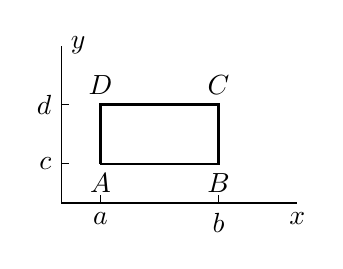
\begin{tikzpicture}
\draw(0,0)--++(3,0)node[below]{$x$};
\draw(0,0)--++(0,2)node[right]{$y$};
\draw[thick](0.5,0.5)node[below]{$A$}--++(1.5,0)node[below]{$B$}--++(0,0.75)node[above]{$C$}--++(-1.5,0)node[above]{$D$}--++(0,-0.75);
\draw(0.5,0)node[below]{$a$}--++(0,0.1);
\draw(2,0)node[below]{$b$}--++(0,0.1);
\draw(0,0.5)node[left]{$c$}--++(0.1,0);
\draw(0,1.25)node[left]{$d$}--++(0.1,0);
\end{tikzpicture}
\end{subfigure}%
\begin{subfigure}{0.5\textwidth}
\centering
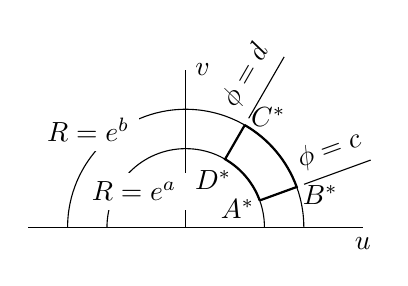
\begin{tikzpicture}
\draw(-2,0)--(2.25,0)node[below]{$u$};
\draw(0,0)--(0,2)node[right]{$v$};
\draw([shift={(0:1)}]0,0) arc (0:180:1);
\draw([shift={(0:1.5)}]0,0) arc (0:180:1.5);
\draw(20:1.6)--(20:2.5)node[pos=0.5,shift={(110:0.3)},rotate=20]{$\phi=c$};
\draw(60:1.6)--(60:2.5)node[pos=0.5,shift={(150:0.3)},rotate=60]{$\phi=d$};
\draw(20:0.7)node[]{$A^*$};
\draw(60:0.7)node[]{$D^*$};
\draw[thick] ([shift={(20:1)}]0,0) arc (20:60:1) --++(60:0.5)node[shift={(0.3,0.1)}]{$C^*$} ([shift={(60:1.5)}]0,0)  arc (60:20:1.5)node[shift={(0.3,-0.1)}]{$B^*$}--(20:1);
\draw(145:0.8)node[fill=white]{$R=e^a$};
\draw(135:1.75)node[fill=white]{$R=e^b$};
\end{tikzpicture}
\end{subfigure}%
\caption{نقش \عددی{w=e^z}}
\label{شکل_نقش_قوت_نمائی}
\end{figure}

بنیادی پٹی \عددی{-\pi<y\le \pi} پوری \عددی{w} سطح  (جو منفی حقیقی محور پر کٹی ہوئی ہوئی ہو گی) پر عکس ہو گی۔مزید ہر \عددی{y=c} اور \عددی{y=c+2\pi} لکیروں کے درمیان افقی پٹی  پوری \عددی{w} سطح پر عکس ہو گی۔یہ \عددی{e^z} کی دوریت کی بدولت ہے جس کا خیالی دوری عرصہ \عددی{i2\pi} ہے۔

مساوات \حوالہ{مساوات_نقش_قوت_نمائی_ب} کے تحت، افقی پٹی \عددی{0\le y\le \pi} بالائی نصف \عددی{w} سطح پر عکس ہوتی ہے۔سرحد \عددی{y=0} مثبت  \عددی{u} محور پر عکس ہوتی ہے جبکہ لکیر \عددی{y=\pi} منفی \عددی{u} محور پر عکس ہوتی ہے۔قطع \عددی{0} تا \عددی{i\pi} کا عکس نصف دائرہ \عددی{\abs{w}=1,\, v\ge 0} ہو گا۔پٹی کی بائیں نصف \عددی{(x\le 0)} حصے کا عکس \عددی{\abs{w}\le 1,\, v\ge 0} اور دائیں نصف \عددی{(x\ge 0)} حصہ  اس نصف دائرہ \عددی{\abs{w}=1}  کی بیرون پر بالائی نصف \عددی{w} مستوی پر عکس ہو گا (شکل \حوالہ{شکل_نقش_قوت-نمائی_ب})۔
\begin{figure}
\centering
\begin{subfigure}{0.5\textwidth}
\centering
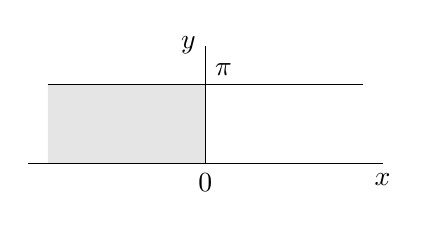
\begin{tikzpicture}
\fill[fill=gray!20!white](-2,0)--(0,0)node[below]{$0$}--(0,1)--(-2,1)--(-2,0);
\draw(-2.25,0)--(2.25,0)node[below]{$x$};
\draw(0,0)--(0,1.5)node[left]{$y$};
\draw(-2,1)--(2.,1);
\draw(0,1)node[above right]{$\pi$};
\end{tikzpicture}
\end{subfigure}%
\begin{subfigure}{0.5\textwidth}
\centering
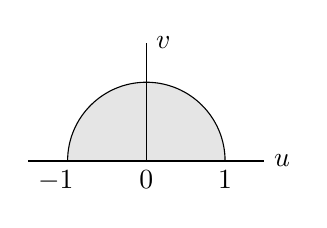
\begin{tikzpicture}
\fill[fill=gray!20!white]([shift={(0:1)}]0,0) arc (0:180:1)--(1,0)node[below]{$1$};
\draw([shift={(0:1)}]0,0) arc (0:180:1);
\draw(-1.5,0)--(1.5,0)node[right]{$u$};
\draw(0,0)node[below]{$0$}--++(0,1.5)node[right]{$v$};
\draw(-1,0)node[below,xshift={(-0.15cm)}]{$-1$};
\end{tikzpicture}
\end{subfigure}%
\caption{نقش \عددی{w=e^z}}
\label{شکل_نقش_قوت-نمائی_ب}
\end{figure}

چونکہ قوت نمائی تفاعل کا الٹ  تعلق \اصطلاح{قدرتی لوگارتھم}\فرہنگ{لوگارتھم!قدرتی} \عددی{w=u+iv=\ln z}  ہے لہٰذا قدرتی لوگارتھم کی محافظ زاویہ نقش کی خواص، متذکرہ بالا میں \عددی{z} اور \عددی{w} سطحوں کی کردار  الٹ کرنے سے  قوت نمائی تفاعل کی خواص سے حاصل کی جا سکتی ہیں۔ یوں صدر قیمت \عددی{w=\Ln z}، (منفی حقیقی محور پر کٹی ہوئی)  \عددی{z} مستوی کو \عددی{w} مستوی کی افقی پٹی \عددی{-\pi<v\le \pi} پر عکس کرتی ہے۔مزید خواص پر اگلے حصے کے مثال \حوالہ{مثال_نقش_لوگارتھمی_ریمان_سطح} میں غور کیا جائے گا۔

\اصطلاح{سائن تفاعل}\فرہنگ{سائن!تفاعل} (حصہ \حوالہ{حصہ_تحلیلی_تکونیاتی_ہذلولی}) 
\begin{align}\label{مساوات_محافظ_سائن_الف}
w=u+iv=\sin z=\sin x\cosh y+i\cos x\sinh y
\end{align}
جہاں
\begin{align}\label{مساوات_محافظ_سائن_ب}
u=\sin x\cosh y,\quad v=\cos x\sinh y
\end{align}
دوری ہیں۔یوں پوری \عددی{xy} مستوی پر مساوات \حوالہ{مساوات_محافظ_سائن_ب} ہرگز ایک ایک مطابقتی نہیں ہے۔ہمیں \عددی{z} کو لامتناہی نصف پٹی
 \عددی{S:-\tfrac{\pi}{2}\le x\le \tfrac{\pi}{2}} کے اندر رہنے کا پابند کرنا ہو گا۔چونکہ \عددی{f'(z)=\cos z} نقطہ \عددی{z=\mp \tfrac{\pi}{2}} پر صفر کے برابر ہے لہٰذا نقش ان دو نقطوں پر محافظ زاویہ نہیں ہو گا۔مساوات \حوالہ{مساوات_محافظ_سائن_ب} سے ہم دیکھتے ہیں کہ \عددی{S} کی سرحد \عددی{u} محور میں  عکس  ہو گی۔\عددی{x} محور کا قطع \عددی{-\tfrac{\pi}{2}\le x\le \tfrac{\pi}{2}} محور \عددی{u} کی قطع \عددی{-1\le u\le 1}  پر عکس ہو گا، لکیر \عددی{x=-\tfrac{\pi}{2}} کا عکس \عددی{u\le -1,\,\, v=0} اور  لکیر \عددی{x=\tfrac{\pi}{2}}  کا عکس \عددی{u\ge 1,\,\, v=0} ہو گا۔قطع \عددی{y=c>0,-\tfrac{\pi}{2}\le x\le \tfrac{\pi}{2}} کا عکس بالائی نصف \عددی{w} مستوی کی قطع مکافی
\begin{align*}
u=\cosh c\sin x,\quad v=\sinh c\cos x
\end{align*}
یعنی
\begin{align}\label{مساوات_نقش_قطع_مکافی}
\frac{u^2}{\cosh^2 c}+\frac{v^2}{\sinh^2 c}=1
\end{align}
پر ہو گا۔قطع \عددی{y=-c,-\tfrac{\pi}{2}\le x\le \tfrac{\pi}{2}\,\,(c>0)}   قطع مکافی مساوات \حوالہ{مساوات_نقش_قطع_مکافی} کی نچلی نصف حصے پر عکس ہو گی۔قطع مکافی کے ماسکہ  جو \عددی{c} کے تابع نہیں ہیں \عددی{w=\mp 1} پر پائے جائیں گے۔یوں \عددی{c} تبدیل کرنے سے ہمیں ہم ماسکہ قطع مکافی حاصل ہوں گے۔مستطیل خطہ \عددی{-\tfrac{\pi}{2}<x<\tfrac{\pi}{2}, \, -c<y<c}  یوں قطع مکافی مساوات \حوالہ{مساوات_نقش_قطع_مکافی} کی اندرون پر عکس ہو گا؛ البتہ دھیان رہے کہ جیسا شکل \حوالہ{شکل_نقش_سائن} میں دکھایا گیا ہے، مستطیل کی سرحد کا عکس قطع مکافی اور \عددی{u} محور کے دو قطعات ہوں گے (جہاں \عددی{c=1} ہے)۔مستطیل کی سرحد کی  انتصابی حصوں پر نقطوں کے عکس جوڑیوں میں ہم مکان نقطے ہوں گے۔  بالخصوص \عددی{B^*=F^*} اور \عددی{C^*=E^*} ہوں گے۔
\begin{figure}
\centering
\begin{subfigure}{0.5\textwidth}
\centering
\begin{tikzpicture}
\draw(-1.5,0)--(2,0)node[right]{$x$};
\draw(0,-1)--(0,1.5)node[right]{$y$};
\draw(-1,-0.75)node[below]{$E$}--++(2,0)node[below]{$F$}--++(0,1.5)node[above]{$B$}--++(-2,0)node[above]{$C$}--++(0,-1.5);
\draw(0,-0.75)node[below left]{$-1$};
\draw(0,0.75)node[above left]{$1$};
\draw(-1,0)node[above left]{$D$}node[below left]{$-\tfrac{\pi}{2}$};
\draw(1,0)node[above right]{$A$}node[below right]{$\tfrac{\pi}{2}$};
\end{tikzpicture}
\end{subfigure}%
\begin{subfigure}{0.5\textwidth}
\centering
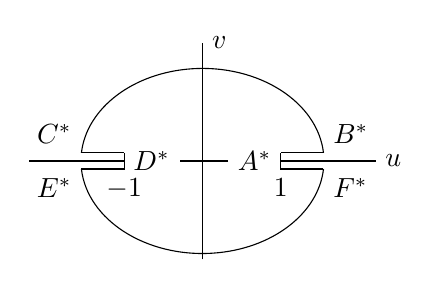
\begin{tikzpicture}
\pgfmathsetmacro{\lx}{1.543}
\pgfmathsetmacro{\ly}{1.1752}
\pgfmathsetmacro{\ang}{5}
\draw(1,0)--++(1.2,0)node[right]{$u$};
\draw(-1,0)--++(-1.2,0);
\draw(0,-1.25)--(0,1.5)node[right]{$v$};
\draw([shift={(\ang:\lx cm and \ly cm)}]0,0) arc (\ang:180-\ang:\lx cm and \ly cm);
\draw([shift={(180+\ang:\lx cm and \ly cm)}]0,0) arc (180+\ang:360-\ang:\lx cm and \ly cm);
\draw(\ang:\lx cm and \ly cm)node[above right]{$B^*$}--++(-0.543,0)coordinate(kT);
\draw(-\ang:\lx cm and \ly cm)node[below right]{$F^*$}--++(-0.543,0)node[below]{$1$}--(kT);
\draw(180-\ang:\lx cm and \ly cm)node[above left]{$C^*$}--++(0.543,0)coordinate(kTT);
\draw(180+\ang:\lx cm and \ly cm)node[below left]{$E^*$}--++(0.543,0)node[below]{$-1$}--(kTT);
\draw(1,0)node[left](kkA){$A^*$};
\draw(-1,0)node[right](kkD){$D^*$};
\draw(kkA)--(kkD);
\end{tikzpicture}
\end{subfigure}%
\caption{نقش \عددی{w=\sin z}}
\label{شکل_نقش_سائن}
\end{figure}

مستطیل خطہ \عددی{-\pi<x<\pi,\, c<y<d\, (c>0)} کا نقش قطع مکافی جھلی ہو گی جو منفی \عددی{v} محور پر کٹی ہو گی (شکل \حوالہ{شکل_نقش_سائن_پٹی})۔سیدھی لکیریں \عددی{x=c} جہاں \عددی{-\tfrac{\pi}{2}<c<\tfrac{\pi}{2}} ہے کے نقش ہم ماسکہ قطع زائد ہوں گی جو متذکرہ بالا قطع مکافی کو زاویہ قائمہ پر قطع کریں گی۔   
\begin{figure}
\centering
\begin{subfigure}{0.5\textwidth}
\centering
\begin{tikzpicture}
\draw(-1.5,0)--(2,0)node[right]{$x$};
\draw(-1.5,0)node[below]{$-\pi$}--++(0,0.1);
\draw(1.5,0)node[below]{$\pi$}--++(0,0.1);
\draw(0,0)node[ocirc]{}node[below]{$0$}--++(0,2)node[right]{$y$};
\draw(-1.5,0.75)node[below]{$A$}--++(3,0)node[below]{$B$}--++(0,0.5)node[above]{$C$}--++(-3,0)node[above]{$D$}--++(0,-0.5);
\draw(0,1.25)node[above left]{$1$};
\end{tikzpicture}
\end{subfigure}%
\begin{subfigure}{0.5\textwidth}
\centering
\begin{tikzpicture}
\pgfmathsetmacro{\lx}{1.543}
\pgfmathsetmacro{\ly}{1.1752}
\pgfmathsetmacro{\lxx}{1.2947}
\pgfmathsetmacro{\lyy}{0.8223}
\pgfmathsetmacro{\ang}{5}
%
\draw[name path=kA](0,0) circle (\lx cm and \ly cm);
\draw[name path=kB](0,0) circle (\lxx cm and \lyy cm);
\path[name path=kC](-0.1,0)--++(0,-1.2);
\path[name path=kD](0.1,0)--++(0,-1.2);
\fill[fill=white](-0.1,0)--++(0,-1.2)--++(0.2,0)--++(0,1.2)--++(-0.2,0);
\draw[name intersections={of=kA and kC, by=kPA},name intersections={of=kB and kC,by=kPB}] (kPA)--(kPB);
\draw[name intersections={of=kA and kD, by=kPA},name intersections={of=kB and kD,by=kPB}] (kPA)--(kPB);
\draw(0,-0.7)node[above](kUP){$A^*=B^*$};
\draw(0,-1.295)node[below](kLW){$D^*=C^*$};
\draw(-1.75,0)--(1.75,0)node[right]{$u$};
\draw(kLW)--(kUP)--(0,1.5)node[right]{$v$};
\draw(0,0)node[ocirc]{};
\draw(-1,0)node[ocirc]{}node[below,xshift={(0.2)}]{$-1$};
\draw(1,0)node[ocirc]{}node[below]{$1$};
\end{tikzpicture}
\end{subfigure}%
\caption{نقش \عددی{w=\sin z}}
\label{شکل_نقش_سائن_پٹی}
\end{figure}
 
\عددی{z} کی \عددی{\tfrac{\pi}{2}} اکائیاں دائیں  مستقیم حرکت کے بعد سائن تفاعل لینے سے \اصطلاح{کوسائن تفاعل}\فرہنگ{کوسائن!تفاعل}
\begin{align}\label{مساوات_نقش_کوسائن_تفاعل}
w=\cos z=\sin\big(z+\frac{\pi}{2}\big)
\end{align}
کا نقش حاصل ہوتا ہے۔

\اصطلاح{ہذلولی تفاعل}\فرہنگ{ہذلولی!تفاعل}
\begin{align}\label{مساوات_نقش_ہذلولی_سائن_تفاعل}
w=\sinh z=-i\sin (iz)
\end{align}
لکھی جا سکتی ہے۔یوں گھڑی کی سمت میں \عددی{\tfrac{\pi}{2}} زاویہ گھمانے \عددی{t=iz} کے بعد نقش \عددی{p=\sin t} لے کر اس کو گھڑی کی الٹ سمت  \عددی{w=-ip} گھمانے سے درکار ہذلولی نقش حاصل ہوتا ہے۔

اسی طرح درج ذیل تبادل
\begin{align}\label{مساوات_نقش_ہذلولی_کوسائن_تفاعل}
w=\cosh z=\cos (iz)
\end{align}
گھمانے \عددی{t=iz} کے بعد نقش \عددی{w=\cos t} کے مترادف ہے۔ 

%========================
\ابتدا{مثال}\شناخت{مثال_نقش_ہذلولی_کوسائن_عکس-لامتناہی_پٹی}\quad \موٹا{نصف لامتناہی پٹی کا نصف سطح پر نقش}\\
نصف لامتناہی پٹی \عددی{x\ge 0, 0\le y\le \pi} (شکل \حوالہ{شکل_مثال_نقش_ہذلولی_کوسائن_عکس-لامتناہی_پٹی}) کا عکس مساوات \حوالہ{مساوات_نقش_ہذلولی_کوسائن_تفاعل} میں دیے گئے نقش کی صورت میں دریافت کریں۔\\
حل:\quad ہم \عددی{w=u+iv} لیتے ہیں۔چونکہ \عددی{\cosh 0=1} کے برابر ہے لہٰذا \عددی{z=0} کو عکس \عددی{w=1} ہو گا۔حقیقی مثبت \عددی{z=x\ge 0} کے لئے \عددی{\cosh z} حقیقی ہے جو \عددی{1} سے شروع ہو کر، \عددی{x} بڑھانے سے، بتدریج بڑھتا ہے۔ یوں مثبت \عددی{x} محور \عددی{u} محور کے حصہ \عددی{u\ge 1} پر عکس ہوتا ہے۔ خالص خیالی \عددی{z=iy} کے لئے \عددی{\cosh iy=\cos y} ہو گا لہٰذا پٹی کی بائیں سرحد \عددی{1\ge u\ge -1} پر عکس ہو گی۔نقطہ \عددی{z=i\pi} کا عکس
\begin{align*}
w=\cosh i\pi=\cos \pi=-1
\end{align*} 
ہو گا۔پٹی کی بالائی سرحد پر \عددی{y=\pi} ہے اور چونکہ \عددی{\sin \pi=0} کے برابر ہے لہٰذا سرحد کا یہ حصہ \عددی{u\le -1} پر عکس ہو گا۔یوں پٹی کی سرحد \عددی{u} محور پر عکس ہو گی۔یہ آسانی سے دیکھا جا سکتا ہے کہ پٹی کی اندرون بالائی نصف \عددی{w} مستوی پر عکس ہو گی اور  کہ یہ نقش ایک ایک مطابقتی ہے۔
\begin{figure}
\centering
\begin{subfigure}{0.5\textwidth}
\centering
\begin{tikzpicture}
\draw(0,0)--(2.5,0)node[below]{$x$};
\draw(0,0)node[ocirc]{}node[left]{$A$}--++(0,1.5)node[left]{$y$};
\draw(0,1)node[ocirc]{}node[left]{$\pi$}node[above right]{$B$}--++(2.5,0);
\end{tikzpicture}
\end{subfigure}%
\begin{subfigure}{0.5\textwidth}
\centering
\begin{tikzpicture}
\draw(-1.5,0)--(1.5,0)node[below]{$u$};
\draw(0,0)node[ocirc]{}node[below]{$0$}--++(0,1.5)node[left]{$v$};
\draw(-1,0)node[ocirc]{}node[below,xshift={(-0.1cm)}]{$-1$}node[above]{$B^*$};
\draw(1,0)node[ocirc]{}node[below]{$1$}node[above]{$A^*$};
\end{tikzpicture}
\end{subfigure}%
\caption{نقش برائے مثال \حوالہ{مثال_نقش_ہذلولی_کوسائن_عکس-لامتناہی_پٹی}}
\label{شکل_مثال_نقش_ہذلولی_کوسائن_عکس-لامتناہی_پٹی}
\end{figure}
\انتہا{مثال}
%====================
\ابتدا{مثال}\شناخت{مثال_نقش_حرارت_پٹی}\quad \موٹا{سرحدی شرائط مسئلہ}\\
مثال \حوالہ{مثال_نقش_ہذلولی_کوسائن_عکس-لامتناہی_پٹی} میں دی گئی پٹی میں برقرار حال (وقت پر غیر منحصر) درجہ حرارت \عددی{T(x,y)} پر غور کریں۔پٹی کی سرحد پر درجہ حرارت درج ذیل ہے۔
\begin{align*}
T&=T_0 \quad \text{\RL{قطع $\,0\,$ تا $\,i\pi\,$ پر}}\\
T&=0\quad \text{\RL{بالائی اور نچلی سرحد پر}}
\end{align*}

\begin{figure}
\centering
\begin{subfigure}{0.5\textwidth}
\centering
\begin{tikzpicture}
\draw(0,0)--(2.5,0)node[below]{$x$};
\draw(0,0)node[below]{$0$}--++(0,1.5)node[left]{$y$};
\draw(0,1)node[ocirc]{}node[left]{$\pi$}--++(2.5,0);
\draw(0,0.5)node[left]{$T=T_0$};
\draw(1.25,0)node[below]{$T=0$};
\draw(1.25,1)node[above]{$T=0$};
\end{tikzpicture}
\end{subfigure}%
\begin{subfigure}{0.5\textwidth}
\centering
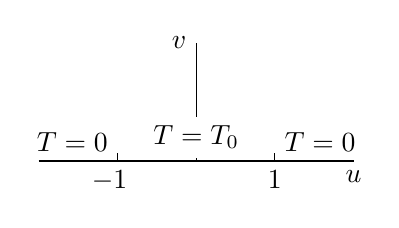
\begin{tikzpicture}
\draw(-2,0)--(2,0)node[below]{$u$};
\draw(0,0)node[shift={(0,0.3)},fill=white]{$T=T_0$}--++(0,1.5)node[left]{$v$};
\draw(-1,0)node[below,xshift={(-0.1cm)}]{$-1$}node[above left]{$T=0$}--++(0,0.1);
\draw(1,0)node[below]{$1$}node[above right]{$T=0$}--++(0,0.1);
\end{tikzpicture}
\end{subfigure}%
\caption{سرحدی شرائط برائے مثال \حوالہ{مثال_نقش_حرارت_پٹی}}
\label{شکل_مثال_نقش_حرارت_پٹی}
\end{figure}

حل:حراری مساوات برقرار حال کی صورت میں  لاپلاس مساوات (حصہ \حوالہ{حصہ_جزوی_مخفی_قوہ})
\begin{align*}
\nabla^{\,2}T=\frac{\partial^{\,2}T}{\partial x^2}+\frac{\partial^{\,2}T}{\partial y^2}=0
\end{align*}
 کی صورت اختیار کرتی ہے۔ہمیں اس مساوات کا ایسا حل درکار ہے جو دی گئی سرحدی شرائط  کو مطمئن کرتا ہو۔

ہم پٹی کو مساوات \حوالہ{مساوات_نقش_ہذلولی_کوسائن_تفاعل} کی مدد سے بالائی نصف مستوی پر عکس کرتے ہیں۔چونکہ قطع \عددی{0\le y\le \pi} کا عکس \عددی{-1\le u \le 1} ہے لہٰذا سرحدی شرائط کو \عددی{w} مستوی میں درج ذیل لکھا جا سکتا ہے (شکل \حوالہ{شکل_مثال_نقش_حرارت_پٹی})۔
\begin{align*}
T&=T_0\quad \text{\RL{قطع $-1$ تا $1$}}\\
T&=0\quad \text{\RL{محور کا باقی حصہ}}
\end{align*}
تحلیلی تفاعل کے حقیقی اور خیالی اجزاء  لاپلاس مساوات کے حل ہوتے ہیں۔ہمیں ایسا ہی تفاعل \عددی{T(u,v)}، جو ان سرحدی شرائط کو مطمئن کرتا ہو، بالائی نصف \عددی{w} مستوی میں دریافت کرنا ہے۔ہم درج ذیل تفاعل پر غور کرتے ہیں۔
\begin{gather}
\begin{aligned}\label{مساوات_نقش_حراری_مثال_تفاعل_الف}
\Ln(w+1)&=\ln\abs{w+1}+i\phi_1,\quad \phi_1=\phase{w+1}=\tan^{-1}\frac{v}{u+1}\\
\Ln(w-1)&=\ln\abs{w-1}+i\phi_2,\quad \phi_2=\phase{w-1}=\tan^{-1}\frac{v}{u-1}
\end{aligned}
\end{gather}
چونکہ \عددی{\phi_1(u,v)} اور \عددی{\phi_2(u,v)} ہارمونی تفاعل ہیں لہٰذا \عددی{\phi_2-\phi_1} بھی ہارمونی تفاعل ہو گا۔اگر \عددی{w=u} حقیقی اور \عددی{-1} سے چھوٹا ہو، تب \عددی{\phi_2-\phi_1=\pi-\pi=0} ہو گا۔وقفہ \عددی{-1<u<1} میں حقیقی \عددی{w=u} کی صورت میں \عددی{\phi_2-\phi_1=\pi-0=\pi} ہو گا، اور حقیقی \عددی{w=u>1} کی صورت میں \عددی{\phi_2-\phi_1=0-0=0} ہو گا۔یوں  بالائی نصف مستوی \عددی{v>0} میں تفاعل
\begin{align}\label{مساوات_نقش_حراری_مثال_پٹی}
T(u,v)=\frac{T_0}{\pi}(\phi_2-\phi_1)
\end{align}
ہارمونی ہو گا اور یہ \عددی{w} سطح میں سرحدی شرائط کو مطمئن کرے گا۔چونکہ \عددی{\tan \phi_1=\tfrac{v}{u+1}} اور \عددی{\tan \phi_2=\tfrac{v}{u-1}} ہیں لہٰذا 
\begin{align*}
\tan(\phi_2-\phi_1)=\frac{\tan \phi_2-\tan \phi_1}{1+\tan\phi_1\tan\phi_2}=\frac{2v}{u^2+v^2-1}
\end{align*}
لکھا جا سکتا ہے۔یوں مساوات \حوالہ{مساوات_نقش_حراری_مثال_پٹی} درج ذیل صورت اختیار کرتی ہے۔
\begin{align}\label{مساوات_نقش_حراری_مثال_پٹی_ب}
T(u,v)=\frac{T_0}{\pi} \tan^{-1}\frac{2v}{u^2+v^2-1}
\end{align}

تفاعل \عددی{w=\cosh z} اس پٹی کو نصف مستوی \عددی{v\ge 0} پر نقش کرتا ہے اور  ہمارے پاس
\begin{align*}
w=u+iv=\cosh (x+iy)=\cosh x\cos y+i\sinh x\sin y
\end{align*}
ہے جس کے حقیقی اور خیالی اجزاء علیحدہ علیحدہ کرنے سے درج ذیل ملتا ہے۔
\begin{align*}
u=\cosh x\cos y,\quad v=\sinh x\sin y
\end{align*}
ان \عددی{u} اور \عددی{v} کے ساتھ یوں مساوات \حوالہ{مساوات_نقش_حراری_مثال_پٹی_ب} میں
\begin{align*}
u^2+v^2-1=\cosh^2 x\cos^2 y+\sinh^2 x\sin^2 y-1=\sinh^2x-\sin^2y
\end{align*}
ہو گا۔مساوات \حوالہ{مساوات_نقش_حراری_مثال_پٹی_ب} میں درج بالا تعلق اور \عددی{v} کا تعلق پر کرنے سے
\begin{align*}
T^*(x,y)=\frac{T_0}{\pi}\tan^{-1} \frac{2\sinh x\sin y}{\sinh^2 x-\sin^2 y}
\end{align*}
ملتا ہے۔ اب شمار کنندہ اور نسب نما بالترتیب تفاعل \عددی{(\sinh x+i\sin y)^2} کے  حقیقی اور خیالی حصے ہیں لہٰذا ہم درج ذیل لکھ سکتے ہیں۔
\begin{align*}
T^*(x,y)=\frac{T_0}{\pi} \phase{[(\sinh x+i\sin y)^2]}=\frac{2T_0}{\pi} \phase{(\sinh x+i\sin y)}
\end{align*}
یوں ہمارے مسئلے کا حل 
\begin{align}
T^*(x,y)=\frac{2T_0}{\pi} \tan^{-1} \frac{\sin y}{\sinh x}
\end{align}
ہو گا۔یہ تفاعل ہماری پٹی کی اندرون میں ہارمونی ہے (مسئلہ \حوالہ{مسئلہ_نقش_اور_ہارمونی_تفاعل}) اور یہ دی گئی سرحدی شرائط کو مطمئن کرتا ہے۔یقیناً \عددی{y=0} یا \عددی{y=\pi} پر \عددی{T^*=0} ہے اور \عددی{x=0} پر \عددی{T^*=T_0} ہے۔ ہم حرارت خط (جن پر یکساں حرارت ہو گی) درج ذیل خطوط ہوں گے۔
\begin{align*}
\frac{\sin y}{\sinh x}=\text{مستقل}
\end{align*}
\انتہا{مثال}
%============================

مثال \حوالہ{مثال_نقش_حرارت_پٹی} میں تفاعل \عددی{w=u(x,y)+iy(x,y)}، جو نصف مستوی کو دیے گئے خطے پر نقش کرتا ہے، کی استعمال سے حقیقی مخفی قوہ  \عددی{T(u,v)} کا عکس حقیقی مخفی قوہ \عددی{T^*(x,y)} حاصل کیا گیا۔مخلوط مخفی قوہ کی استعمال سے کئی مسئلوں کا حل نسبتاً آسان ہو جاتا ہے، یعنی ایسا مخلوط تحلیلی تفاعل \عددی{F(w)} لینے سے  کہ حقیقی تفاعل \عددی{T(u,v)}، تفاعل \عددی{F(w)} کا حقیقی یا خیالی جزو ہو اور \عددی{T} کی بجائے \عددی{F} کا تبادل لیا جائے۔ظاہر ہے کہ \عددی{T} کا جوڑی دار ہارمونی تفاعل (حصہ \حوالہ{حصہ_تحلیلی_کوشی_ریمان_مساوات_لاپلاس} کا آخر دیکھیں) حاصل کرنے سے  مخلوط مخفی قوہ \عددی{F}  حاصل ہو گا۔  آئیں  "مخلوط مخفی قوہ کی ترکیب" \فرہنگ{ترکیب!مخلوط مخفی قوہ}\فرہنگ{مخفی قوہ!مخلوط، ترکیب}\فرہنگ{complex potentials!method} گزشتہ مثال کی صورت میں دیکھیں۔مخلوط مخفی قوہ پر  باب \حوالہ{باب_مخلوط_تفاعل_اور_نظریہ_مخفی_قوہ} میں غور کیا جائے گا۔

%======================
\ابتدا{مثال}\quad \موٹا{مخلوط مخفی قوہ}\\
مساوات \حوالہ{مساوات_نقش_حراری_مثال_تفاعل_الف} سے ہم دیکھتے ہیں کہ مثال \حوالہ{مثال_نقش_حرارت_پٹی} میں حقیقی مخفی قوہ (مساوات \حوالہ{مساوات_نقش_حراری_مثال_پٹی})
\begin{align*}
T(u,v)=\frac{T_0}{\pi}(\phi_2-\phi_1)
\end{align*}
درحقیقت مخلوط مخفی قوہ
\begin{align}\label{مساوات_نقش_مخلوط_مخفی_قوہ_مثال_الف}
T(w)=\frac{T_0}{\pi}[\Ln(w-1)-\Ln(w+1)]=\frac{T_0}{\pi}\Ln\frac{w-1}{w+1}
\end{align}
کا خیالی جزو ہے۔مثال \حوالہ{مثال_نقش_حرارت_پٹی} میں تفاعل نقش
\begin{align*}
w=\cosh z=\frac{1}{2}(e^z+e^{-z})
\end{align*}
ہے جس سے ہم دیکھتے ہیں کہ مساوات \حوالہ{مساوات_نقش_مخلوط_مخفی_قوہ_مثال_الف} میں
\begin{align*}
\frac{w-1}{w+1}=\frac{\cosh z-1}{\cosh z+1}=\frac{e^z+e^{-z}-2}{e^z+e^{-z}+2}=\frac{(e^{\frac{z}{2}}+e^{-\frac{z}{2}})^2}{(e^{\frac{z}{2}}+e^{-\frac{z}{2}})^2}=\tanh^2 \frac{z}{2}
\end{align*}
ہو گا۔اس کو مساوات \حوالہ{مساوات_نقش_مخلوط_مخفی_قوہ_مثال_الف} میں میں پر کرتے ہوئے اور \عددی{F(w(z))} کو \عددی{F^*(z)} سے اور \عددی{\tanh \tfrac{z}{2}} کو \عددی{H} سے  ظاہر کرتے ہوئے  درج ذیل ملتا ہے۔
\begin{align}
F^*(z)=\frac{T_0}{\pi}\Ln \tanh^2\frac{z}{2}=\frac{2T_0}{\pi}\Ln \tanh \frac{z}{2}=\frac{2T_0}{\pi} \Ln h
\end{align}
مساوات \حوالہ{مساوات_مخلوط_لوگارتھم_ب} کی استعمال سے اس کو
\begin{align}\label{مساوات_نقش_ایک_حل}
F^*(z)=\frac{2T_0}{\pi} \Ln H=\frac{2T_0}{\pi} \big(\ln\abs{H}+i\tan^{-1}\frac{\text{\RL{خیالی $H\,$}}}{\text{\RL{حقیقی $H\,$}}}\big)
\end{align}
لکھا جا سکتا ہے۔ \عددی{F^*(z)} مثال \حوالہ{مثال_نقش_حرارت_پٹی} میں مخلوط مخفی قوہ ہے اور اس کا خیالی جزو ہمارے مسئلے کا حل ہے۔\عددی{H} کو قوت نمائی تفاعل کی مدد سے لکھ کر
\begin{align}\label{مساوات_نقش_حل_دوسری_شکل}
H=\frac{\sinh x+i\sin y}{\cosh x+\cos y}
\end{align}
لکھا جا سکتا ہے جس کو مساوات \حوالہ{مساوات_نقش_ایک_حل} کے ساتھ ملا کر
\begin{align*}
T^*(x,y)=\text{\RL{خیالی $F^*(z)\,$}}=\frac{2T_0}{\pi}\tan^{-1} \frac{\sin y}{\sinh x}
\end{align*}
حاصل ہوتا  ہے جو مثال \حوالہ{مثال_نقش_حرارت_پٹی} کی نتیجہ کے عین مطابق ہے۔

مزید مساوات \حوالہ{مساوات_نقش_حل_دوسری_شکل} سے
\begin{align*}
\abs{H}^2=\frac{\sinh^2x+\sin^2y}{(\cosh x+\cos y)^2}
\end{align*}
لکھا جا سکتا ہے۔یوں مساوات \حوالہ{مساوات_نقش_ایک_حل} میں ہم دیکھتے ہیں کہ \عددی{F^*(z)} کا حقیقی جزو درج ذیل صورت اختیار کرتا ہے۔
\begin{align*}
S^*(x,y)=\text{\RL{حقیقی $F^*(z)\,$}}=\frac{T_0}{\pi}\ln \frac{\sinh^2x+\sin^2y}{(\cosh x+\cos y)^2}
\end{align*}
منحنیات \عددی{S^*=\text{مستقل}} ہم حرارت خطوط \عددی{T^*=\text{مستقل}} کو زاویہ قائمہ پر قطع کرتی ہیں اور یوں حرارت انہیں خطوط کی راہ  پر بہاو کرتی ہے۔مخلوط مخفی قوہ کی استعمال سے ہمیں دونوں خطوط حاصل ہوتے ہیں۔
\انتہا{مثال}
%============================

\حصہء{سوالات}
سوال \حوالہ{سوال_نقش_قوت_نمائی_الف} تا سوال \حوالہ{سوال_نقش_قوت_نمائی_ب} میں زیر نقش \عددی{w=e^z} دیے گئے تفاعل کا عکس تلاش کریں۔ عکس کو \عددی{w} سطح پر دکھائیں۔

%===============
\ابتدا{سوال}\شناخت{سوال_نقش_قوت_نمائی_الف}\quad
$-1<x<1,\quad -\tfrac{\pi}{2}<y<\tfrac{\pi}{2}$\\
جواب:\quad
\عددی{w=\abs{w}\phase{w}=e^{x+iy}} سے 
$e^{-1}<\abs{w}<e^1,\quad \abs{\phase{w}}<\tfrac{\pi}{2}$
ملتا ہے۔
\انتہا{سوال}
%======================
\ابتدا{سوال}\quad
$0<x<4,\quad 0<y<\pi$\\
جواب:\quad
$e^0<\abs{w}<e^4,\quad 0<\phase{w}<\pi$
\انتہا{سوال}
%=====================
\ابتدا{سوال}\quad
$0<x<1,\quad -1<y<1$\\
جواب:\quad
$e^0<\abs{w}<e^1,\quad -1<\phase{w}<1$
\انتہا{سوال}
%=====================
\ابتدا{سوال}\quad
$-\pi<x<2,\quad -\tfrac{\pi}{2}<y<3$\\
جواب:\quad
$e^{-\pi}<\abs{w}<e^2,\quad -\tfrac{\pi}{2}<\phase{w}<3$
\انتہا{سوال}
%=====================
\ابتدا{سوال}\quad
$-2\le x\le 3,\quad -\tfrac{\pi}{2}\le y\le \tfrac{\pi}{2}$\\
جواب:\quad
$e^{-2}\le \abs{w}\le e^3,\quad -\tfrac{\pi}{2}\le \phase{w}\le \tfrac{\pi}{2}$
\انتہا{سوال}
%=====================
\ابتدا{سوال}\شناخت{سوال_نقش_قوت_نمائی_ب}\quad
$0< x\le 2.2,\quad -\tfrac{\pi}{2}\le y< \pi$\\
جواب:\quad
$e^{0}< \abs{w}\le e^{2.2},\quad -\tfrac{\pi}{2}\le \phase{w}< \pi$
\انتہا{سوال}
%=====================
\ابتدا{سوال}\quad
ایسا تحلیلی تفاعل تلاش کریں جو ربع اول میں ایسا خطہ جس کی سرحد مثبت \عددی{x}، مثبت \عددی{y} اور قطع زائد \عددی{xy=\tfrac{\pi}{2}}  ہو کو بالائی نصف سطح پر عکس کرتا ہو۔ اشارہ۔ پہلے اس خطے کو افقی پٹی پر عکس کریں۔\\
جواب:\quad
\عددی{t=z^2} اس خطے کو \عددی{0<\text{\RL{خیالی $t\,$}}<\pi} پٹی  پر عکس کرتی ہے اور \عددی{w=e^t} اس پٹی کو بالائی نصف مستوی پر عکس کرتی ہے لہٰذا درکار تفاعل \عددی{w=e^{\,z^2}} ہے۔
\انتہا{سوال}
%=======================
سوال \حوالہ{سوال_نقش_سائن_تفاعل_الف} تا سوال \حوالہ{سوال_نقش_سائن_تفاعل_ب} میں دیے تفاعل کا عکس زیر نقش \عددی{w=\sin z} تلاش کریں۔عکس کو \عددی{w} سطح پر دکھائیں۔

%===============
\ابتدا{سوال}\شناخت{سوال_نقش_سائن_تفاعل_الف}\quad
$0<x<\tfrac{\pi}{2},\quad 0<y<2$\\
\انتہا{سوال}
%=========================
\ابتدا{سوال}\quad
$-\tfrac{\pi}{2}<x<\tfrac{\pi}{2},\quad 1<y<2$\\
جواب:\quad
بالائی نصف مستوی میں وہ خطہ کس کی سرحد درج ذیل قطع مکافی ہوں۔
\begin{align*}
\frac{u^2}{\cosh^2 2}+\frac{v^2}{\sinh^2 2}=1, \quad \frac{u^2}{\cosh^2 1}+\frac{v^2}{\sinh^2 1}=1
\end{align*}
\انتہا{سوال}
%=========================
\ابتدا{سوال}\quad
$-\tfrac{\pi}{2}<x<\tfrac{\pi}{2},\quad 0<y<1$\\
\انتہا{سوال}
%=========================
\ابتدا{سوال}\شناخت{سوال_نقش_سائن_تفاعل_ب}\quad
$0<x<2\pi,\quad 1<y<2$\\
جواب:\quad
بالائی نصف مستوی میں وہ چھلا جس کی سرحد درج ذیل قطع مکافی ہوں اور جو مثبت خیالی محور پر کٹا ہوا ہو۔
\begin{align*}
\frac{u^2}{\cosh^2 2}+\frac{v^2}{\sinh^2 2}=1, \quad \frac{u^2}{\cosh^2 1}+\frac{v^2}{\sinh^2 1}=1
\end{align*}
\انتہا{سوال}
%=========================
\ابتدا{سوال}\quad
زیر نقش \عددی{w=\sin z} سیدھی لکیریں \عددی{x=0,\mp \tfrac{\pi}{6},\mp\tfrac{\pi}{3},\mp\tfrac{\pi}{2}} کا عکس تلاش کریں اور انہیں \عددی{w} مستوی پر دکھائیں۔\\
جواب:\quad
$x=0: u=0,\quad x=\mp \tfrac{\pi}{6}: 4u^2-\tfrac{4}{3}v^2=1$

\انتہا{سوال}
%======================
\ابتدا{سوال}\quad
نقش \عددی{w=\cosh z} کو نقش \عددی{w=\sin z}، گھومنے اور مستقیم حرکت کی صورت میں لکھیں۔\\
جواب:\quad
$\cosh z=\cos (iz)=\sin(iz+\tfrac{\pi}{2})$
\انتہا{سوال}
%===================
\ابتدا{سوال}\شناخت{سوال_نقش_لوگارتھمی_عکس_الف}\quad
دکھائیں کہ نقش \عددی{w=\Ln\tfrac{z-1}{z+1}} بالائی نصف مستوی کو افقی پٹی \عددی{0\le \text{\RL{خیالی $w\,$}}\le \pi} پر عکس کرتا ہے (شکل \حوالہ{شکل_سوال_نقش_لوگارتھمی_عکس_الف})۔
\begin{figure}
\centering
\begin{subfigure}{0.5\textwidth}
\centering
\begin{tikzpicture}
\draw(-2.5,0)node[above]{$A$}node[below]{$(\infty)$}--(2.5,0)node[above]{$E$}node[below]{$(\infty)$};
\draw(-1,0)node[below]{$-1$}--++(0,0.1)node[above]{$B$};
\draw(0,0)node[below]{$0$}--++(0,0.1)node[above]{$C$};
\draw(1,0)node[below]{$1$}--++(0,0.1)node[above]{$D$};
\draw(0,-0.75)node[]{مستوی $z\,$};
\end{tikzpicture}
\end{subfigure}%
\begin{subfigure}{0.5\textwidth}
\centering
\begin{tikzpicture}
\draw(-1.5,0)--(0,0)node[ocirc]{}node[below]{$0$}node[above]{$E^*=A^*$}--(1.5,0);
\draw(-1.5,1)--(0,1)node[ocirc]{}node[below]{$C^*$}node[above]{$i\pi$}--(1.5,1);
\draw(-1.5,0.5)node[]{$D^*(\infty)$};
\draw(1.5,0.5)node[]{$B^*(\infty)$};
\draw(0,-0.75)node[]{مستوی $w\,$};
\end{tikzpicture}
\end{subfigure}%
\caption{شکل برائے سوال \حوالہ{سوال_نقش_لوگارتھمی_عکس_الف}}
\label{شکل_سوال_نقش_لوگارتھمی_عکس_الف}
\end{figure}
\انتہا{سوال}
%=======================
سوال \حوالہ{سوال_نقش_حرارت_الف} تا سوال \حوالہ{سوال_نقش_حرارت_ث} میں دھات کی پتلی تختی دکھائی گئی ہے جس کی دونوں سطحیں حاجز شدہ ہیں جبکہ کنارے دیے گئے درجہ حرارت پر رکھے گئے ہیں۔برقرار حال درجہ حرارت \عددی{T(x,y)} تلاش کریں۔ 
\begin{figure}
\centering
\begin{subfigure}{0.33\textwidth}
\centering
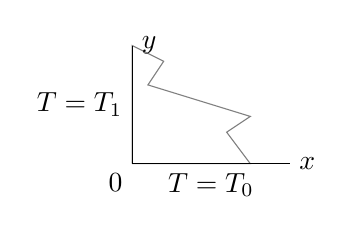
\begin{tikzpicture}
\draw[gray] plot coordinates {(0,0) (1.5,0) (1.2,0.4) (1.5,0.6)  (0.2,1)(0.4,1.3) (0,1.5) (0,0)};
\draw(0,0)node[below left]{$0$}--(2,0)node[right]{$x$}node[below,pos=0.5]{$T=T_0$};
\draw(0,0)--(0,1.5)node[right]{$y$}node[left,pos=0.5]{$T=T_1$};
\end{tikzpicture}
\caption*{(الف)}
\end{subfigure}%
\begin{subfigure}{0.33\textwidth}
\centering
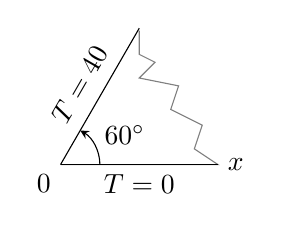
\begin{tikzpicture}
%\draw[thick] (0,0)grid (2,2);
%\draw[thin,gray,step=0.1](0,0) grid (2,2);
%
\draw[gray] plot coordinates {(0,0) (2,0) (1.7,0.2) (1.8,0.5) (1.4,0.7) (1.5,1) (1,1.1) (1.2,1.3) (1,1.4) (1,1.7)};
\draw(0,0)node[below left]{$0$}--(2,0)node[right]{$x$}node[below,pos=0.5]{$T=\SI{0}{\celsius}$};
\draw(0,0)--(60:2)node[pos=0.5,shift={(150:0.3)},rotate=60]{$T=\SI{40}{\celsius}$};
\draw[-stealth] ([shift={(0:0.5)}]0,0) arc (0:60:0.5);
\draw(25:0.9)node[]{$60^{\circ}$};
\end{tikzpicture}
\caption*{(ب)}
\end{subfigure}%
\begin{subfigure}{0.33\textwidth}
\centering
\begin{tikzpicture}
%\draw[thick] (0,0)grid (2,2);
%\draw[thin,gray,step=0.1](0,0) grid (2,2);
%
\draw[gray]  ([shift={(0:2)}]0,0) arc (0:45:2)--(0,0)--cycle;
\draw[thick]([shift={(0:2)}]0,0) arc (0:45:2);
\draw(22.5:2.3)node[rotate=-67.5]{\RL{حاجز شدہ}};
\draw(0,0)--(2,0)node[right]{$x$}node[below,pos=0.5]{$T=\SI{0}{\celsius}$};
\draw(0,0)--(45:2)node[pos=0.5,shift={(150:0.3)},rotate=45]{$T=\SI{100}{\celsius}$};
\draw[-stealth] ([shift={(0:0.5)}]0,0) arc (0:45:0.5);
\draw(20:0.9)node[]{$45^{\circ}$};
\end{tikzpicture}
\caption*{(پ)}
\end{subfigure}
\begin{subfigure}{0.33\textwidth}
\centering
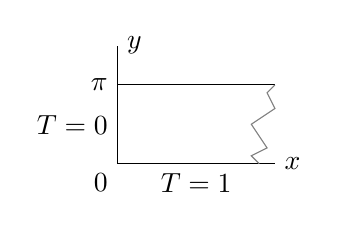
\begin{tikzpicture}
%\draw[thick] (0,0)grid (2,2);
%\draw[thin,gray,step=0.1](0,0) grid (2,2);
%
%\draw[gray] plot coordinates {(0,0) (2,0) (1.7,0.2) (1.8,0.5) (1.4,0.7) (1.5,1) (1,1.1) (1.2,1.3) (1,1.4) (1,1.7)};
\draw(0,0)node[below left]{$0$}--(2,0)node[right]{$x$}node[below,pos=0.5]{$T=\SI{1}{\celsius}$};
\draw(0,0)--(0,1.5)node[pos=0.33,left]{$T=\SI{0}{\celsius}$}node[right]{$y$};
\draw(0,1)node[left]{$\pi$}--(2,1);
\draw[gray] plot coordinates {(2,1) (1.9,0.9) (2,0.7) (1.7,0.5) (1.9,0.2) (1.7,0.1) (1.8,0)};
\end{tikzpicture}
\caption*{(ت)}
\end{subfigure}%
\begin{subfigure}{0.33\textwidth}
\centering
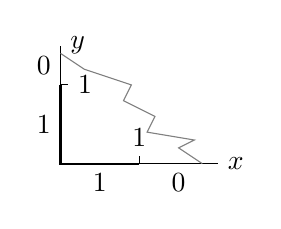
\begin{tikzpicture}
%\draw[thick] (0,0)grid (2,2);
%\draw[thin,gray,step=0.1](0,0) grid (2,2);
%
\draw(0,0)--(2,0)node[right]{$x$};
\draw(0,0)--(0,1.5)node[right]{$y$};
\draw(1,0)--++(0,0.1)node[above]{$1$};
\draw(0,1)--++(0.1,0)node[right]{$1$};
\draw[thick](0,1)--(0,0)--(1,0);
\draw(0.5,0)node[below]{$\SI{1}{\celsius}$};
\draw(1.5,0)node[below]{$\SI{0}{\celsius}$};
\draw(0,0.5)node[left]{$\SI{1}{\celsius}$};
\draw(0,1.25)node[left]{$\SI{0}{\celsius}$};
\draw[gray] plot coordinates {(0,1.4) (0.3,1.2) (0.9,1) (0.8,0.8) (1.2,0.6) (1.1,0.4) (1.7,0.3) (1.5,0.2) (1.8,0)};
\end{tikzpicture}
\caption*{(ٹ)}
\end{subfigure}%
\begin{subfigure}{0.33\textwidth}
\centering
\begin{tikzpicture}
%\draw[thick] (0,0)grid (2,2);
%\draw[thin,gray,step=0.1](0,0) grid (2,2);
%
\draw(0,0)--(2,0)node[right]{$x$};
\draw(0,0)--(0,1.5)node[right]{$y$};
\draw[thick]([shift={(0:0.5)}]0,0) arc (0:90:0.5);
\draw[thick]([shift={(0:1)}]0,0) arc (0:90:1);
\draw(0.75,0)node[below]{$\SI{0}{\celsius}$};
\draw(0,0.75)node[left]{$\SI{100}{\celsius}$};
\draw[stealth-](60:1) to [out=40,in=180]++(0.5,0.3)coordinate(kA)node[right]{\RL{حاجز شدہ}};
\draw[stealth-] (30:0.5) to [out=60,in=180] (kA);
\end{tikzpicture}
\caption*{(ث)}
\end{subfigure}
\caption{دھات کی تختی برائے سوال \حوالہ{سوال_نقش_حرارت_الف}-الف تا سوال \حوالہ{سوال_نقش_حرارت_الف}-ث}
\label{شکل_سوال_نقش_حرارت_الف}
\end{figure}

%================
\ابتدا{سوال}\شناخت{سوال_نقش_حرارت_الف}\quad
شکل \حوالہ{شکل_سوال_نقش_حرارت_الف}-الف\\
جواب:\quad
$T=T_0+\tfrac{1}{\pi} (T_1-T_0)\tan^{-1}\tfrac{2xy}{x^2-y^2}=T_0+\tfrac{2}{\pi}(T_1-T_0)\tan^{-1}\tfrac{y}{x}$
\انتہا{سوال}
%=======================
\ابتدا{سوال}\quad
شکل \حوالہ{شکل_سوال_نقش_حرارت_الف}-ب
\انتہا{سوال}
%=======================
\ابتدا{سوال}\quad
شکل \حوالہ{شکل_سوال_نقش_حرارت_الف}-پ\\
جواب:\quad
$T=\tfrac{100}{\pi/4}\tan^{-1}\tfrac{y}{x}$
\انتہا{سوال}
%=======================
\ابتدا{سوال}\quad
شکل \حوالہ{شکل_سوال_نقش_حرارت_الف}-ت
\انتہا{سوال}
%=======================
\ابتدا{سوال}\quad
شکل \حوالہ{شکل_سوال_نقش_حرارت_الف}-ٹ\\
جواب:\quad
$T=\tfrac{1}{\pi} \tan^{-1} \tfrac{4xy}{(x^2+y^2)^2-1}$
\انتہا{سوال}
%=======================
\ابتدا{سوال}\شناخت{سوال_نقش_حرارت_ث}\quad
شکل \حوالہ{شکل_سوال_نقش_حرارت_الف}-ث
\انتہا{سوال}
%=======================

\حصہ{ریمان سطحیں}
ہم نقش 
\begin{align}
w=u+iv=z^2
\end{align}
پر غور کرتے ہیں (حصہ \حوالہ{حصہ_نقش_نقشہ_کشی})۔ یہ نقش محافظ زاویہ ہے ماسوائے نقطہ \عددی{z=0} پر جہاں \عددی{w'=2z} صفر کے برابر ہے۔ یہ نقش نقطہ \عددی{z=0} پر  زاویہ دگنا کرتا ہے۔\عددی{z} مستوی کا دایاں نصف (بشمول مثبت \عددی{y} محور)، منفی \عددی{u} محور پر کٹے ہوئے،  پوری  \عددی{w} مستوی پر ایک ایک مطابقت کے ساتھ عکس ہوتا ہے۔اسی طرح \عددی{z} مستوی کا بایاں نصف (بشمول منفی \عددی{y} محور) کٹے ہوئے  \عددی{w}مستوی پر عکس ہو گا۔

چونکہ ہر \عددی{w\ne 0} نقطہ کے ٹھیک دو مطابقتی \عددی{z} نقطے پائے جاتے ہیں لہٰذا  پوری \عددی{z} مستوی کے لحاظ سے یہ نقش ایک ایک مطابقتی نہیں ہے۔یوں اگر  ایسا ایک  نقطہ \عددی{z_1} ہو تب دوسرا نقطہ \عددی{-z_1} ہو گا۔مثال کے طور پر \عددی{z=i} اور \عددی{z=-i} دونوں کا مطابقتی نقطہ \عددی{w=-1} ہے۔یوں پوری \عددی{z} مستوی کا عکس \عددی{w} مستوی کو دو مرتبہ ڈھانپتا ہے۔ہم کہتے ہیں کہ پوری \عددی{z} مستوی "دوہرا ڈھانپا" \عددی{w} مستوی پر عکس ہوتا ہے۔ہم اپنی سوچ و فکر کو درکار سہارا درج ذیل طریقہ سے دیتے ہیں۔

ہم پوری \عددی{z} مستوی کا \عددی{w} مستوی پر دو مرتبہ عکس کے دونوں حصوں کو ایک دوسرے کے اوپر یوں رکھتے ہیں کہ دایاں نصف \عددی{z} مستوی کا عکس اوپر اور بایاں  نصف \عددی{z} مستوی کا عکس نیچے ہو۔ہم  دائیں نصف \عددی{z} مستوی کو \عددی{D} اور بائیں نصف \عددی{z} مستوی کو \عددی{B} سے ظاہر کرتے ہیں۔یوں \عددی{z} مستوی پر چلتے ہوئے  \عددی{D} سے \عددی{B} جانب جانے  سے مطابقتی نقطہ عکس بالائی سے نچلی چادر پر منتقل ہو گا۔اسی لئے ہم دونوں چادروں کو کٹے ہوئے مقام پر آپس میں جوڑتے ہیں۔دونوں مبدا ایک ہی نقطہ پر جڑتے ہیں۔یوں \اصطلاح{ریمان سطح}\فرہنگ{ریمان!سطح}\حاشیہب{Riemann surface}\فرہنگ{Riemann!surface} حاصل ہوتی ہے جسے شکل \حوالہ{شکل_نقش_ریمان_سطح_اور_تقسیمی_نقطہ} میں دکھایا گیا ہے۔ ریمان سطح پر ہر نقطہ \عددی{w\ne 0}، منطبق مقام پر، دو مرتبہ ظاہر ہو گا جبکہ مبدا صرف ایک مرتبہ نظر آئے گا۔تفاعل \عددی{w=z^2} اب پوری \عددی{z} سطح کو اس ریمان سطح پر،  ایک ایک مطابقت سے، عکس کرتا ہے، اور یہ نقش محافظ زاویہ ہے ماسوائے \عددی{w=0} یعنی  \اصطلاح{تقسیمی نقطہ}\فرہنگ{تقسیمی نقطہ}\فرہنگ{نقطہ!تقسیمی}\حاشیہب{branch point}\فرہنگ{branch point} پر جہاں \عددی{w'=0} ہے (شکل \حوالہ{شکل_نقش_ریمان_سطح_اور_تقسیمی_نقطہ})۔ ایسا تقسیمی نقطہ جو دو چادروں کو ملاتا ہو \ترچھا{یک رتبی} کہلاتا ہے۔ \عددی{n} چادروں کو ملانے والا تقسیمی نقطہ \عددی{n-1} \موٹا{رتبی} کہلائے گا۔
\begin{figure}
\centering
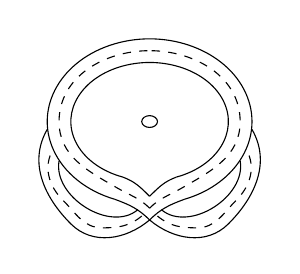
\begin{tikzpicture}
\pgfmathsetmacro{\kdy}{0.3}
\pgfmathsetmacro{\kx}{1}
\pgfmathsetmacro{\ky}{0.75}
\pgfmathsetmacro{\kkx}{1+\kdy}
\pgfmathsetmacro{\kky}{0.75+0.5*\kdy}
\pgfmathsetmacro{\kang}{20}
\pgfmathsetmacro{\kangA}{30}
%grid
%\draw[thick] (-2,-2) grid (2,2);
%\draw[thin,gray,step=0.1] (-2,-2) grid (2,2);
%
\draw(0,0) circle (0.1cm and 3/4*0.1 cm);
\draw([shift={(-90+\kang:\kx cm and \ky cm)}]0,0) arc (-90+\kang:270-\kang:\kx cm and \ky cm);
\draw(-90+\kang:\kx cm and \ky cm) to [out=180+\kang,in=45] (-90:\ky cm+0.2cm);
\draw(-90-\kang:\kx cm and \ky cm) to [out=-\kang,in=135] (-90:\ky cm+0.2cm);
%
\draw([shift={(-90+\kang:\kx cm+\kdy cm and \ky cm+\kdy cm)}]0,0) arc (-90+\kang:270-\kang:\kx cm+\kdy cm and \ky cm+\kdy cm);
\draw(-90+\kang:\kx cm+\kdy cm and \ky cm+\kdy cm) to [out=180+\kang,in=45] (-90:\ky cm+\kdy cm+0.2cm)coordinate(kC);
\draw(-90-\kang:\kx cm+\kdy cm and \ky cm+\kdy cm) to [out=-\kang,in=135] (-90:\ky cm+\kdy cm+0.2cm)coordinate(kD);
%
\draw(0.15,-1.12)  to [out=-40,in=-80] (1.15,-0.5);
\draw(kD) to  [out=-40, in =-135] (1,-1.3) to [out=45,in=-60] (1.3,-0.1);
\draw(-0.15,-1.12)  to [out=180+40,in=180+80] (-1.15,-0.5);
\draw(kD) to  [out=180+40, in =-45] (-1,-1.3) to [out=180-45,in=180+60] (-1.3,-0.1);
%dashed
\draw[dashed](kD)++(0,0.15) to [out=45,in=-150] (0.4,-0.85) to [out=30,in=-90] (1.15,0) to [out=90,in=0] (0,0.9);
\draw[dashed](kD)++(0,0.15) to [out=180-45,in=-30] (-0.4,-0.85) to [out=180-30,in=-90] (-1.15,0) to [out=90,in=180] (0,0.9);
\draw[dashed](0.1,-1.2) to [out=-40,in=180] (0.6,-1.35) to [out=0,in=-135] (1.1,-1)to [out=45,in=-60] (1.225,-0.35);
\draw[dashed](-0.1,-1.2) to [out=-140,in=0] (-0.6,-1.35) to [out=180,in=-45] (-1.1,-1)to [out=135,in=180+60] (-1.225,-0.35);
\end{tikzpicture}%
\caption{ریمان سطح اور تقسیمی نقطہ}
\label{شکل_نقش_ریمان_سطح_اور_تقسیمی_نقطہ}
\end{figure}

ہم اب دوہرا قیمت تعلق
\begin{align}\label{مساوات_نقش_جذر_تفاعل_الف}
w=\sqrt{z}
\end{align} 
پر غور کرتے ہیں۔ہر \عددی{z=0} کے مطابقتی دو \عددی{w}  قیمتیں پائی جائیں گی جن میں سے ایک \اصطلاح{صدر قیمت} ہو گی۔اگر ہم \عددی{z} مستوی کی جگہ متذکرہ بالا دو چادری ریمان سطح  لیں تب ہر مخلوط عدد \عددی{z\ne 0} منطبق مقامات پر دو مرتبہ ظاہر کیا جائے گا۔ہم ان میں سے ایک نقطہ کو صدر قیمت کا مطابقتی نقطہ  تصور کرتے ہیں (مثلاً بالائی چادر میں نقطہ) اور دوسرے نقطہ کو دوسری قیمت کا مطابقتی نقطہ تصور کرتے ہیں۔یوں مساوات \حوالہ{مساوات_نقش_جذر_تفاعل_الف} کا تعلق، واحد قیمت تعلق بن جاتا ہے یعنی مساوات \حوالہ{مساوات_نقش_جذر_تفاعل_الف} ریمان سطح پر نقطوں کا تفاعل ہو گا، اور یوں سطح پر \عددی{z} کی کسی بھی استمراری حرکت کا \عددی{w} مستوی پر عکس کا مطابقتی استمراری حرکت پایا جائے گا۔یہ تفاعل صدر قیمت کی مطابقتی چادر کو  \عددی{w} مستوی کی دائیں نصف حصے پر  عکس کرتا ہے جبکہ دوسری چادر کو \عددی{w} مستوی کی بائیں نصف پر عکس کرتا ہے۔

آئیں چند اہم مثال دیکھیں۔

%===================
\ابتدا{مثال}\quad \موٹا{\عددی{\sqrt[\leftroot{-2}\uproot{2}n]{z}} کی ریمان سطح}\\
درج ذیل تعلق کے لئے ہمیں \عددی{n} چادر کی ریمان سطح درکار ہو گی جس کا \عددی{z=0} پر   \عددی{n-1} رتبی تقسیمی نقطہ پایا جائے گا۔
\begin{align}
\sqrt[\leftroot{-2}\uproot{2}n]{z}\quad \quad \quad n=3,2,\cdots
\end{align}
ان میں سے ایک چادر صدر قیمت کی مطابقتی چادر ہو گی جبکہ باقی \عددی{n-1} چادر باقی \عددی{n-1} قیمتوں کے مطابقتی ہوں گے۔
\انتہا{مثال}
%=====================  
\ابتدا{مثال}\شناخت{مثال_نقش_لوگارتھمی_ریمان_سطح}\quad \موٹا{قدرتی لوگارتھم کی ریمان سطح}\\
ہر \عددی{z\ne 0} کے لئے درج ذیل  تعلق لامتناہی قیمتی ہے۔
\begin{align}\label{مساوات_نقش_ریمان_سطح_لوگارتھم}
w=\ln z=\Ln z+i2n\pi\quad \quad \quad (n=0,\mp1,\mp2,\cdots,\quad z\ne 0)
\end{align}
یوں مساوات \حوالہ{مساوات_نقش_ریمان_سطح_لوگارتھم} لامتناہی تعداد کی چادروں پر مشتمل ریمان سطح پر تفاعل ہو گا۔تفاعل \عددی{w=\Ln z} ان میں سے ایک چادر  کا مطابقتی ہے۔اس چادر پر \عددی{z} کی دلیل \عددی{\theta} کا سعت \عددی{-\pi<\theta\le \pi} ہو گا (حصہ \حوالہ{حصہ_تحلیلی_لوگارتھم_عمومی_طاقت})۔ منفی حقیقی محور چادر کو کاٹ کر جوڑ کی بالائی کنارے کو  اگلی چادر کی نچلے کنارے کے ساتھ منسلک کیا جائے گا جو سعت \عددی{\pi<\theta\le 3\pi} کا مطابقتی یعنی تفاعل \عددی{w=\Ln z+i2\pi} کا مطابقتی ہو گا۔اس طرح  مساوات \حوالہ{مساوات_نقش_ریمان_سطح_لوگارتھم} میں \عددی{n} کی ہر قیمت کا، ان لامتناہی چادروں میں سے،  واحد ایک مطابقتی چادر پایا جائے گا۔تفاعل \عددی{w=\Ln z} مطابقتی چادر کو \عددی{w} سطح میں  افقی پٹی \عددی{-pi<v\le \pi} پر عکس کرتا ہے۔اگلی چادر پڑوسی پٹی \عددی{\pi<v\le 3\pi} پر عکس ہو گی، وغیرہ وغیرہ۔یوں تفاعل \عددی{w=\ln z} مطابقتی ریمان سطح کی تمام چادروں کو  پوری \عددی{w} مستوی پر، ایک ایک مطابقت سے، عکس کرتا ہے۔
\انتہا{مثال}
%====================
\ابتدا{مثال}\شناخت{مثال_نقش_ہوائی_پترا}\quad \موٹا{ہوائی پترا}\\
آئیں درج ذیل نقش پر غور کرتے ہیں جو \اصطلاح{ہوائی حرکیات}\فرہنگ{ہوائی حرکیات}\فرہنگ{حرکیات!ہوائی}\حاشیہب{aerodynamics}\فرہنگ{aerodynamics} کے لئے انتہائی اہم ہے (نیچے تفصیل دی گئی ہے)۔
\begin{align}\label{مساوات_نقش_ہوائی_حرکیات_الف}
w=z+\frac{1}{z}\quad \quad \quad (z\ne 0)
\end{align}
چونکہ 
\begin{align*}
w'=1-\frac{1}{z^2}=\frac{(z+1)(z-1)}{z^2}
\end{align*}
کے برابر ہے لہٰذا یہ نقش محافظ زاویہ ہے، ماسوائے  نقطہ \عددی{z=1} اور نقطہ  \عددی{z=-1} پر جہاں \عددی{w'=0} ہے۔یہ نقطے بالترتیب \عددی{w=2} اور \عددی{w=-2} کے مطابقتی نقطے ہیں۔مساوات \حوالہ{مساوات_نقش_ہوائی_حرکیات_الف} سے درج ذیل حاصل ہوتا ہے۔
\begin{align}
z=\frac{w}{2}\mp \sqrt{\frac{w^2}{4}-1}=\frac{w}{2}\mp\frac{1}{2}\sqrt{(w+2)(w-2)}
\end{align}
اس طرح \عددی{w=2} اور \عددی{w=-2} تفاعل \عددی{z=z(w)} کے  یک رتبی تقسیمی نقطے ہیں۔کسی بھی \عددی{w\,(\ne2,\ne-2)} قیمت کے مطابقتی دو \عددی{z} قیمتیں ہوں گی لہٰذا مساوات \حوالہ{مساوات_نقش_ہوائی_حرکیات_الف} مستوی \عددی{z} کو دو چادر کی ریمان سطح پر، ایک ایک مطابقت سے، عکس کرتی ہے اور یہ دو چادر \عددی{w=-2} تا \عددی{w=2} آپس میں صلیبی جڑی ہیں (شکل \حوالہ{شکل_مثال_نقش_ہوائی_پترا})۔ہم \عددی{z=re^{i\theta}} لیتے ہوئے \عددی{r=\text{مستقل}} اور \عددی{\theta=\text{مستقل}} کے عکس تلاش کرتے ہیں۔مساوات \حوالہ{مساوات_نقش_ہوائی_حرکیات_الف} سے
\begin{figure}
\centering
\begin{subfigure}{0.5\textwidth}
\centering
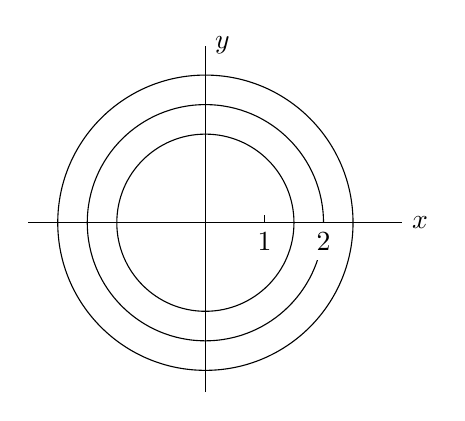
\begin{tikzpicture}
\pgfmathsetmacro{\kS}{3/4}
\draw(-2.25,0)--(2.5,0)node[right]{$x$};
\draw(0,-2.15)--(0,2.25)node[right]{$y$};
\draw(0,0) circle (1.5*\kS);
\draw(0,0) circle (2*\kS);
\draw(0,0) circle (2.5*\kS);
\draw(1*\kS,0)node[below]{$1$}--++(0,0.1);
\draw(2*\kS,0)node[below,fill=white]{$2$};
\end{tikzpicture}
\end{subfigure}%
\begin{subfigure}{0.5\textwidth}
\centering
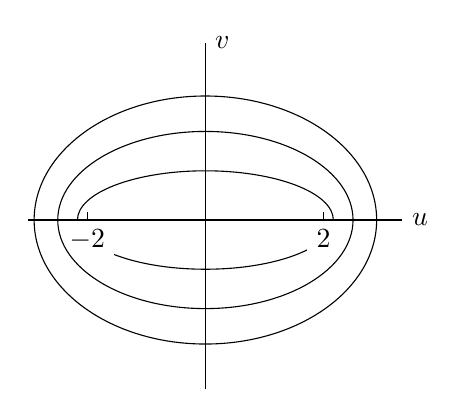
\begin{tikzpicture}
\pgfmathsetmacro{\kS}{3/4}
\pgfmathsetmacro{\kA}{\kS*(1.5+1/1.5)}
\pgfmathsetmacro{\kB}{\kS*(1.5-1/1.5)}
\pgfmathsetmacro{\kkA}{\kS*(2+1/2)}
\pgfmathsetmacro{\kkB}{\kS*(2-1/2)}
\pgfmathsetmacro{\kkkA}{\kS*(2.5+1/2.5)}
\pgfmathsetmacro{\kkkB}{\kS*(2.5-1/2.5)}
\draw(-2.25,0)--(2.5,0)node[right]{$u$};
\draw(0,-2.15)--(0,2.25)node[right]{$v$};
\draw(0,0) circle (\kA cm and \kB cm);
\draw(2*\kS,0)node[below,fill=white]{$2$}--++(0,0.1);
\draw(-2*\kS,0)node[below,fill=white]{$-2$}--++(0,0.1);
\draw(0,0) circle (\kkA cm and \kkB cm);
\draw(0,0) circle (\kkkA cm and \kkkB cm);
\end{tikzpicture}
\end{subfigure}%
\caption{شکل برائے مثال \حوالہ{مثال_نقش_ہوائی_پترا}}
\label{شکل_مثال_نقش_ہوائی_پترا}
\end{figure}
%
\begin{align*}
w=u+iv=re^{i\theta}+\frac{1}{r}e^{-i\theta}=\big(r+\frac{1}{r}\big)\cos \theta+i\big(r-\frac{1}{r}\big)\sin\theta
\end{align*}
حاصل ہو گا جس کے حقیقی اور خیالی اجزاء علیحدہ علیحدہ کرتے ہوئے 
\begin{align}\label{مساوات_نقش_ہوائی_حرکیات_ب}
u=\big(r+\frac{1}{r}\big)\cos \theta,\quad v=\big(r-\frac{1}{r}\big)\sin\theta
\end{align}
ملتا ہے جن سے درج ذیل لکھا جا سکتا ہے۔
\begin{align*}
\frac{u^2}{a^2}+\frac{v^2}{b^2}=1,\quad \quad a=r+\frac{1}{r},\quad b=\abs{r-\frac{1}{r}}
\end{align*}
یوں \عددی{r=\text{مستقل}} دائروں کا عکس قطع مکافی ہوں گے جن کی صدر محور \عددی{u} اور \عددی{v} ہوں گی اور ان کی لمبائیاں بالترتیب \عددی{2a} اور \عددی{2b} ہوں گی۔ چونکہ \عددی{a^2-b^2=4} متغیر \عددی{r} کا تابع نہیں ہے لہٰذا یہ قطع مکافی ہم ماسکہ ہوں گی اور اس کے ماسکہ \عددی{w=-2} اور \عددی{w=2} پر ہوں  گے۔اکائی دائرہ \عددی{r=1} کا عکس \عددی{w=-2} تا \عددی{w=2} قطع ہو گا۔ہر \عددی{r\ne 1} کی صورت میں رداس \عددی{r} اور رداس \عددی{\tfrac{1}{r}} کے دائرے  \عددی{w} مستوی میں ریمان سطح کی دو چادروں پر ہم مقام (ایک جیسے)  قطع مکافی پر عکس ہوں گے۔یوں اکائی دائرہ \عددی{\abs{z}=1} کی اندرون ایک چادر پر اور اس کی بیرون دوسری چادر پر ہو گی۔

مزید مساوات \حوالہ{مساوات_نقش_ہوائی_حرکیات_ب} سے
\begin{align}
\frac{u^2}{\cos^2\theta}-\frac{v^2}{\sin^2\theta}=-4
\end{align}
حاصل کیا جا سکتا ہے۔یوں سیدھی لکیریں \عددی{\theta=\text{مستقل}} متذکرہ بالا قطع مکافی کی قائمہ الزاویہ، قطع زائد پر عکس ہوں گی۔حقیقی محور یعنی مبدا سے نکلتی سیدھی لکیریں \عددی{\theta=0} اور \عددی{\theta=\pi} کا عکس حقیقی محور پر \عددی{w=2} سے \عددی{w=\infty} کے راستے \عددی{w=-2} تک  ہو گا۔\عددی{y}  محور کا عکس  \عددی{v} محور پر ہو گا۔مبدا سے نکلتی کوئی اور سیدھی لکیروں کی جوڑی  \عددی{\theta=\theta_0} اور \عددی{\theta=\theta_0+\pi} ایک ہی قطع زائد کی دو شاخوں پر عکس ہوں گی۔

متذکرہ بالا قطع مکافی کی بیرون تقسیمی نقطہ سے پاک ہے اور \عددی{z} مستوی میں یہ یا تو دائرے کی اندرون اور یا اس کی بیرون کا مطابقتی خطہ ہو گا؛ یہ اس ریمان سطح پر منحصر ہے جس پر یہ خطہ پایا جاتا ہو۔بالخصوص (جیسا ہم ذکر کر چکے ہیں) پوری \عددی{w} مستوی اکائی دائرہ \عددی{\abs{z}=1} کی اندرون یا بیرون کا مطابقتی ہو گا۔

نقش مساوات \حوالہ{مساوات_نقش_ہوائی_حرکیات_الف}  موزوں دائروں کو \اصطلاح{ہوائی پترا}\فرہنگ{ہوائی پترا}\حاشیہب{airfoil}\فرہنگ{airfoil} میں عکس کرتا ہے جس کے پچھلے کنارے کی دھار تیز  اور اندرونی زاویہ صفر ہوتا ہے۔ ان ہوائی پترا کو \اصطلاح{ژکوسکی ہوائی پترا}\فرہنگ{ہوائی پترا!ژکوسکی}\حاشیہب{Joukowski airfoil}\فرہنگ{airfoil!Joukowski} کہتے\حاشیہد{روسی ریاضی دان [1847-1921] نکولائے یگورو وچ ژکوسکی} ہیں۔ چونکہ تیز دھار والی ہوائی پتری درکار  ہوتی ہے لہٰذا وہ دائرہ جو \عددی{z=\mp 1} میں سے ایک نقطہ سے گزرتا ہو کا عکس ہمیں چاہیے ہے۔ ان نقطوں پر نقش غیر محافظ ہے۔ آئیں ہم دائرہ \عددی{C} منتخب کرتے ہیں جو \عددی{z=-1} سے گزرتا ہے اور اس دائرے کی رداس اتنا چنتے ہیں کہ نقطہ \عددی{z=1} دائرے کے اندر ہو۔جیومیٹری کی مدد سے \عددی{z} اور \عددی{\tfrac{1}{z}} سمتیات کا سمتی مجموعہ لینے سے یہ عکس با آسانی حاصل ہو گا (جہاں \عددی{\tfrac{1}{z}} کو \عددی{z} سے حاصل کرنا حصہ \حوالہ{حصہ_نقش_نقشہ_کشی} میں دکھایا گیا ہے)۔حاصل عکس کو شکل \حوالہ{شکل_نقش_ژکوسکی_ہوائی_پترا} میں دکھایا گیا ہے
\begin{figure}
\centering
\begin{subfigure}{0.5\textwidth}
\centering
\begin{tikzpicture}
\draw(-1.5,0)--(2,0)node[below]{$x$};
\draw(0,-1.5)--(0,1.75)node[left]{$y$};
\draw(0.25,0) circle (1.25);
\draw[dashed](0,0) circle (1); 
\draw(-1,0)node[ocirc]{}node[below left]{$-1$};
\draw(1,0)node[ocirc]{}node[below left]{$1$};
\draw(30:1.75)node{$C$};
\end{tikzpicture}
\end{subfigure}%
\begin{subfigure}{0.5\textwidth}
\centering
\begin{tikzpicture}
\draw(-2.25,0)--(0.5,0) (2.2,0)--(2.75,0)node[right]{$u$};
\draw(0,-0.5)--(0,0.1) (0,0.55)--(0,1)node[right]{$v$};
\draw(-2,0) to [out=20,in=180] (0.25,0.5) to [out=0,in=155](2,0.1) to [out=-35,in=90] (2+0.1,0);
\draw(-2,0) to [out=10,in=180] (-0.5,0.2) to [out=0,in=175](2,-0.1) to [out=-5,in=-90] (2+0.1,0);
\draw[dashed](-2,0) to [out=18,in=165]  (2,0);
\draw(-2,0)node[ocirc]{}node[below,xshift={(-0.15cm)}]{$-2$};
\draw(2,0)node[ocirc]{}node[below]{$2$};
\end{tikzpicture}
\end{subfigure}%
\caption{ژکوسکی ہوائی پترا}
\label{شکل_نقش_ژکوسکی_ہوائی_پترا}
\end{figure}
\انتہا{مثال}
%====================

\حصہء{سوالات}

%====================
\ابتدا{سوال}\quad
\عددی{w=\sqrt{z}} لیں۔نقطہ \عددی{z} اکائی دائرے کے گرد دو مرتبہ گھومتا ہے۔اس نقطے کی عکس کی راہ تلاش کریں۔ابتدائی نقطہ \عددی{z=1} لیں۔\\
جواب:\quad
نقطہ \عددی{w} اکائی دائرہ \عددی{\abs{w}=1} کے گرد ایک مرتبہ گھومے گا۔
\انتہا{سوال}
%=========================
\ابتدا{سوال}\شناخت{سوال_نقش_ریمان_سطحیں_ب}\quad
دکھائیں کہ \عددی{\sqrt[\leftroot{-2}\uproot{2}3]{z}} کی ریمان سطح تین چادروں پر مشتمل ہے جس کا دو رتبی تقسیمی نقطہ \عددی{z=0} ہے۔ نقطہ \عددی{z} اکائی دائرے کے گرد تین مرتبہ گھومتا ہے۔یہ نقطہ \عددی{z=1} سے ابتدا کرتا ہے۔اس کے عکس کی راہ تلاش کریں۔
\انتہا{سوال}
%========================
\ابتدا{سوال}\quad
\عددی{\sqrt[\leftroot{-2}\uproot{2}4]{z}} اور \عددی{\sqrt[\leftroot{-2}\uproot{2}5]{z}} کی ریمان سطحوں  پر بھی سوال \حوالہ{سوال_نقش_ریمان_سطحیں_ب} کی طرح تبصرہ کریں۔\\
جواب:\quad
بالترتیب \عددی{4} اور \عددی{5} چادریں۔تقسیمی نقطہ \عددی{z=0} پر ہے۔
\انتہا{سوال}
%=====================
\ابتدا{سوال}\quad
\عددی{\sqrt[\leftroot{-2}\uproot{2}4]{z}} اور \عددی{\sqrt[\leftroot{-2}\uproot{2}5]{z}} کی شکل \حوالہ{شکل_نقش_ریمان_سطح_اور_تقسیمی_نقطہ} کی طرح  ریمان سطحوں کا خاکہ بنائیں جن میں تقسیمی نقطوں کی وضاحت ہو۔
\انتہا{سوال}
%==========================
\ابتدا{سوال}\quad
زیر نقش \عددی{w=z+\tfrac{1}{z}} جھلی \عددی{\tfrac{1}{2}<\abs{z}<1}، \عددی{1<\abs{z}<2} اور \عددی{2<\abs{z}<3} کے عکس تلاش کریں۔\\
جواب:\quad
اندرون قطع مکافی 
$\tfrac{u^2}{(5/2)^2}+\tfrac{v^2}{(3/2)^2}=1$
، دوسری چادر پر اسی قطع مکافی کی اندرون، اس قطع مکافی اور قطع مکافی 
$\tfrac{u^2}{(10/3)^2}+\tfrac{v^2}{(8/3)^2}=1$
کے درمیان جھلی۔
\انتہا{سوال}
%====================
\ابتدا{سوال}\quad
زیر نقش \عددی{w=\ln z} نقطہ \عددی{z} اکائی دائرے کے گرد کئی مرتبہ چکر کاٹتا ہے۔اس نقطے کے عکس کی راہ تلاش کریں۔
\انتہا{سوال}
%=======================
\ابتدا{سوال}\quad
دکھائیں کہ نقش  \عددی{w=\sqrt{(z-1)(z-4)}} کی ریمان سطحہ دو چادروں پر مشتمل ہے  جس  کے تقسیمی نقطے \عددی{z=1} اور \عددی{z=4} ہیں۔مزید دکھائیں کہ ان چادروں کو \عددی{1} تا \عددی{4} لکیر پر کاٹ کر صلیبی جوڑا جائے گا۔\ترچھا{اشارہ۔} قطبی محدد \عددی{z-1=r_1e^{i\theta_1}} اور \عددی{z-4=r_2e^{i\theta_2}} استعمال کریں۔
\انتہا{سوال}
%========================
\ابتدا{سوال}\quad
دکھائیں کہ نقش  \عددی{w=\sqrt{(1-z^2)(4-z^2)}} کی ریمان سطحہ دو چادروں پر مشتمل ہے  جس  کے چار تقسیمی نقطے ہیں۔مزید دکھائیں کہ ان چادروں کو \عددی{x} محور پر لکیر   \عددی{-2\le x\le -1}  اور لکیر \عددی{1\le x\le 2} پر کاٹ کر صلیبی جوڑا جائے گا۔
\انتہا{سوال}
%=========================
سوال \حوالہ{سوال_نقش_ریمان_تقسیمی_نقطے_الف} تا سوال \حوالہ{سوال_نقش_ریمان_تقسیمی_نقطے_ب} میں دیے تفاعل کی ریمان سطحوں  کے تقسیمی نقطے تلاش کریں اور چادروں کی تعداد دریافت کریں۔ 

%======================
\ابتدا{سوال}\شناخت{سوال_نقش_ریمان_تقسیمی_نقطے_الف}\quad
$w=i\sqrt{z}$\\
جواب:\quad 
دو چادر، تقسیمی نقطہ \عددی{z=0} پر ہے۔
\انتہا{سوال}
%=========================
\ابتدا{سوال}\quad
$w=\sqrt{z-i}$
\انتہا{سوال}
%=========================
\ابتدا{سوال}\quad
$w=\sqrt[\leftroot{-2}\uproot{2}3]{z-i}$\\
جواب:\quad
تین چادر، دو رتبی  تقسیمی نقطہ \عددی{z=i} پر ہے۔
\انتہا{سوال}
%=========================
\ابتدا{سوال}\quad
$w=\sqrt[\leftroot{-2}\uproot{2}3]{2z+i3}$
\انتہا{سوال}
%=========================
\ابتدا{سوال}\quad
$w=\sqrt{z^2+1}$\\
جواب:\quad
دو چادر، تقسیمی نقطہ \عددی{\mp i} پر ہے۔
\انتہا{سوال}
%=========================
\ابتدا{سوال}\quad
$w=\sqrt{z(z-1)(z+1)}$
\انتہا{سوال}
%=========================
\ابتدا{سوال}\quad
$w=\sqrt{(z-a)(z-b)},\quad a\ne b$\\
جواب:\quad
دو چادر، تقسیمی نقطے \عددی{a} اور \عددی{b}  پر ہیں۔
\انتہا{سوال}
%=========================
\ابتدا{سوال}\quad
$w=1+z+\sqrt{z}$
\انتہا{سوال}
%=======================
\ابتدا{سوال}\quad
$w=\ln(z-a)$\\
جواب:\quad
چادروں کی تعداد لامتناہی ہے، تقسیمی نقطہ \عددی{a} پر ہے۔
\انتہا{سوال}
%=======================
\ابتدا{سوال}\quad
$w=e^{\sqrt{z}}$
\انتہا{سوال}
%=======================
\ابتدا{سوال}\quad
$w=\sqrt{e^z}$\\
جواب:\quad
دو چادر جو آپس میں جڑے نہیں ہیں۔یوں کوئی تقسیمی نقطہ نہیں پایا جائے گا۔در حقیقت \عددی{\sqrt{e^z}} دو علیحدہ علیحدہ تفاعل \عددی{e^{\tfrac{z}{2}}} اور
 \عددی{-e^{\tfrac{z}{2}}} کو ظاہر کرتا ہے۔
\انتہا{سوال}
%=======================
\ابتدا{سوال}\شناخت{سوال_نقش_ریمان_تقسیمی_نقطے_ب}\quad
$w=\sqrt{\sqrt[\leftroot{-2}\uproot{2}3]{z}-1}$
\انتہا{سوال}
%=======================
